%
% Template Laporan Tugas Akhir Jurusan Informatika Unsyiah 
%
% @author  Kurnia Saputra 
% @version 1.0
% @since 03.02.2016
%
% Template ini telah disesuaikan dengan aturan penulisan tugas akhir yang terdapat pada dokumen Panduan Tugas Akhir FMIPA Unsyiah tahun 2010.
%


% Template pembuatan naskah tugas akhir.
\documentclass{jifhasil}

\tolerance=1
\emergencystretch=\maxdimen
\hyphenpenalty=10000
\hbadness=10000

%\usepackage[a4paper,left=14cm,right=3cm,top=3cm,bottom=5cm]{geometry}

% Daftar pemenggalan suku kata dan istilah dalam LaTeX
%
% Hyphenation untuk Indonesia 
%
% @author  Andreas Febrian
% @version 1.00
% 
% Tambahkan cara pemenggalan kata-kata yang salah dipenggal secara otomatis 
% oleh LaTeX. Jika kata tersebut dapat dipenggal dengan benar, maka tidak 
% perlu ditambahkan dalam berkas ini. Tanda pemenggalan kata menggunakan 
% tanda '-'; contoh:
% menarik
%   --> pemenggalan: me-na-rik
%

\hyphenation{
    % alphabhet A
    a-na-li-sa a-tur 
    a-pli-ka-si 
    android
    % alphabhet B
    ba-ngun-an 
    be-be-ra-pa 
    ber-ge-rak
    ber-ke-lan-jut-an 
    ber-pe-nga-ruh 
    % alphabhet C
    ca-ri
    % alphabhet D
    di-sim-pan di-pim-pin de-ngan da-e-rah di-ba-ngun da-pat di-nya-ta-kan 
    di-sim-bol-kan di-pi-lih di-li-hat de-fi-ni-si
    % alphabhet E
    e-ner-gi eks-klu-sif
    % alphabhet F
    fa-si-li-tas
    foot-print
    % alphabhet G
    ga-bung-an ge-rak
    % alphabhet H
    ha-lang-an
    % alphabhet I
    % alphabhet J
    % alphabhet K
    ke-hi-lang-an
    ku-ning 
    kua-li-tas ka-me-ra ke-mung-kin-an ke-se-pa-ham-an
    % alphabhet L
    ling-kung-an
    % alphabhet M
    me-neng-ah
    meng-a-tas-i me-mung-kin-kan me-nge-na-i me-ngi-rim-kan 
    meng-u-bah meng-a-dap-ta-si me-nya-ta-kan mo-di-fi-ka-si
    meng-a-tur
    mem-pro-mo-si-kan
    me-la-ku-kan
    meng-i-den-ti-fi-ka-si-kan
    % alphabhet N
    nya-ta non-eks-klu-sif
    % alphabhet O
    % alphabhet P
	pe-nye-rap-an 
	pe-ngon-trol
    pe-mo-del-an
    pe-ran  pe-ran-an-nya
    pem-ba-ngun-an pre-si-den pe-me-rin-tah prio-ri-tas peng-am-bil-an 
    peng-ga-bung-an pe-nga-was-an pe-ngem-bang-an 
    pe-nga-ruh pa-ra-lel-is-me per-hi-tung-an per-ma-sa-lah-an 
    pen-ca-ri-an peng-struk-tur-an
    pe-ran-ca-ngan
    plat-form
    patch
    % alphabhet Q
    % alphabhet R
    ran-cang-an
    % alphabhet S
    si-mu-la-si sa-ngat
    smart-phone
    % alphabhet T
    te-ngah
    ter-da-pat
    % alphabhet U
    % alphabhet V
    % alphabhet W
    % alphabhet X
    % alphabhet Y
    % alphabhet Z
    % special
}

% Untuk prefiks pada daftar gambar dan tabel
\usepackage[titles]{tocloft}
\renewcommand\cftfigpresnum{Gambar\  }
\renewcommand\cfttabpresnum{Tabel\   }

\newcommand{\listappendicesname}{DAFTAR LAMPIRAN}
\newlistof{appendices}{apc}{\listappendicesname}
\newcommand{\appendices}[1]{\addcontentsline{apc}{appendices}{#1}}
\newcommand{\newappendix}[1]{\section*{#1}\appendices{#1}}

% Untuk hyperlink dan table of content
\usepackage[hidelinks]{hyperref}
\renewcommand\UrlFont{\rmfamily\itshape} %it's me!
\newlength{\mylenf}
\settowidth{\mylenf}{\cftfigpresnum}
\setlength{\cftfignumwidth}{\dimexpr\mylenf+2em}
\setlength{\cfttabnumwidth}{\dimexpr\mylenf+2em}

% Agar ada tulisan BAB pada TOC
\renewcommand\cftchappresnum{BAB } 
  \cftsetindents{chapter}{0em}{4.5em} %indenting bab
  \cftsetindents{section}{4.5em}{2em}
  \cftsetindents{subsection}{6.5em}{3em}
 
% Agar di TOC setiap angka bab/subbab diakhiri titik

\renewcommand{\cftsecaftersnum}{.}
\renewcommand{\cftsubsecaftersnum}{.}

% Agar setiap angka bab/subbab diakhiri titik
\usepackage{titlesec}
\titlelabel{\thetitle.\quad}

% Agar disetiap caption table dan gambar diakhiri titik
\usepackage[labelsep=period]{caption}

% Untuk Bold Face pada Keterangan Gambar
\usepackage[labelfont=bf]{caption}

% Untuk caption dan subcaption
\usepackage{caption}
\usepackage{subcaption}


% Agar bisa menggunakan warna LaTeX
\usepackage{color} %it's me!

% Agar table yang panjang bisa cut ke next page    %byRennyAdr
\usepackage{longtable}

% Untuk page landscape        %byRennyAdr
\usepackage{pdflscape}
\usepackage{lscape}

% Agar bisa bikin code snippet
\usepackage{listings, lstautogobble} %it's me!


% Warna pada code snippet Java
\definecolor{javared}{rgb}{0.6,0,0} % untuk strings
\definecolor{javagreen}{rgb}{0.25,0.5,0.35} % untuk comments
\definecolor{javapurple}{rgb}{0.5,0,0.35} % untuk keywords
\definecolor{javadocblue}{rgb}{0.25,0.35,0.75} % untuk javadoc

% Warna pada code snippet C/C++
\definecolor{mygray}{rgb}{0.4,0.4,0.4}
\definecolor{mygreen}{rgb}{0,0.8,0.6}
\definecolor{myorange}{rgb}{1.0,0.4,0}

% Sampul Depan
%-----------------------------------------------------------------
% Sampul Depan
%-----------------------------------------------------------------
\judul{RANCANG BANGUN APLIKASI PELAPORAN PENYALURAN GAS LPG 3KG PADA PANGKALAN GAS LPG.}

% nama lengkap
\fullname{Andri Darnius}

% NPM (Nomor Pokok Mahasiswa)
\idnum{1608107010057}

\degree{Sarjana Komputer}

\yearsubmit{AGUSTUS, 2018}

\program{Informatika}

\dept{Informatika}

% Pembimbing Pertama
\firstsupervisor{Rahmad Dawood, S.Kom, M.Sc.}
\firstnip{197203181995121001}

% Pembimbing Kedua
\secondsupervisor{Kurnia Saputra, S.T., M.Sc.}
\secondnip{198003262014041001}

% Ketua Jurusan
\kajur{Dr. Muhammad Subianto, S.Si., M.Si}
\kajurnip{196812111994031005}

% tangal lulus proposal, seminar hasil atau sidang
\approvaldate{Rabu, 21 Agustus 2018}

%-----------------------------------------------------------------
% End of Sampul Depan
%-----------------------------------------------------------------


% Awal dokumen
\usepackage{fancyhdr}
\usepackage{rotating}
% Untuk prefiks pada Daftar Program   
% byRennyAdr
\makeatletter
\begingroup\let\newcounter\@gobble\let\setcounter\@gobbletwo
\globaldefs\@ne \let\c@loldepth\@ne
\newlistof{listings}{lol}{\lstlistlistingname}
\endgroup
\let\l@lstlisting\l@listings
\AtBeginDocument{\addtocontents{lol}{\protect\addvspace{10\p@}}}
\makeatother
\renewcommand{\lstlistoflistings}{\listoflistings}
\renewcommand\cftlistingspresnum{Program~}
\cftsetindents{listings}{1.5em}{7em}

%tab didaftar pustaka -Indah
\setlength{\bibhang}{30pt}

\begin{document}

\cover

\fancyhf{} 

\fancyfoot[C]{\thepage}


\approvalpage

%-----------------------------------------------------------------
% Disini kata pengantar
%-----------------------------------------------------------------
\preface % Note: \preface JANGAN DIHAPUS!


\par Syukur Alhamdulillah penulis panjatkan ke hadirat Allah SWT yang telah melimpahkan rahmat-Nya sehingga penulis dapat menyelesaikan Tugas Akhir yang berjudul \textbf{“Rancang Bangun Aplikasi Pelaporan Penyaluran Gas Lpg 3 Kg Pada Pangkalan Gas Lpg”}. Shalawat dan salam tak lupa pula penulis sanjungkan kepada junjungan kita Nabi Muhammad SAW yang telah menerangi alam ini dengan cahaya keislaman dan ilmu pengetahuan.
\par Tugas Akhir ini merupakan salah satu syarat yang harus dipenuhi untuk memperoleh gelar Sarjana Komputer di Jurusan Informatika, Fakultas Matematika dan Ilmu Pengetahuan Alam, Universitas Syiah Kuala. Penulis menyadari bahwa penulisan Tugas Akhir ini tidak terlepas dari bantuan dan dorongan dari berbagai pihak, baik secara moril maupun materil. Pada kesempatan ini penulis ingin mengucapkan terima kasih kepada:

\begin{enumerate}
	\item{Bapak Dr. Muhammad Subianto, S.Si, M.Si, selaku Ketua Jurusan Informatika Fakultas MIPA Universitas Syiah Kuala.}
	\item{Bapak Irvanizam, S.Si, M.Sc, selaku Dosen Wali.}
	\item{Bapak Rahmad Dawood, S.Kom, M.Sc., selaku dosen pembimbing I dan Bapak Kurnia Saputra, S.T, M.Sc, selaku dosen pembimbing II yang telah banyak memberikan bimbingan dan arahan kepada penulis dalam penyelesaian Proposal Penelitian Tugas Akhir ini.,}
	\item{Seluruh Dosen di Jurusan Informatika Fakultas MIPA, yang tidak bisa disebutkan satu-satu, atas ilmu dan didikannya selama perkuliahan,}
	\item {Staf administrasi Jurusan Informatika yang telah membantu proses administrasi.}
	\item{Dengan tidak mengurangi rasa hormat penulis ucapkan terima kasih sebesar- besarnya kepada Ayahanda Saya Alm. Darnius dan Ibunda saya Ida Nursanti yang tak henti-henti mendukung, memberikan motivasi dan senantiasa mendoakan penulis dari awal masa studi hingga saat ini.}
	\item {Sahabat seperjuangan Riki dan Yusran } 
	\item{Seluruh teman-teman jurusan Informatika Unsyiah angkatan 2014 sampai 2016 yang telah memberikan semangat kepada penulis dalam menyelesaikan Tugas Akhir ini.}
\end{enumerate}


Dengan segala kerendahan hati, penulis mengharapkan semoga tulisan ini
dapat bermanfaat bagi para pembaca, peneliti dan bagi perkembangan ilmu
pengetahuan.

\vspace{0.5cm}


\begin{tabular}{p{7.5cm}c}
	&Banda Aceh, Agustus 2018\\
	&\\
	&\\
	&\textbf{Penulis}
\end{tabular}


%-----------------------------------------------------------------
% TOC menggunakan single space
%-----------------------------------------------------------------
\begin{singlespace}
	\tableofcontents
\end{singlespace}

\addcontentsline{toc}{chapter}{DAFTAR ISI}
\listoftables
\addcontentsline{toc}{chapter}{DAFTAR TABEL}
\listoffigures
\addcontentsline{toc}{chapter}{DAFTAR GAMBAR}

%\renewcommand{\lstlistlistingname}{DAFTAR PROGRAM}
%\lstlistoflistings
%\addcontentsline{toc}{chapter}{DAFTAR PROGRAM}

%\listofappendices
%\addcontentsline{toc}{chapter}{DAFTAR LAMPIRAN}

%-----------------------------------------------------------------
% Daftar Singkatan 
%-----------------------------------------------------------------
%\include{daftar-singkatan}

%-----------------------------------------------------------------
% Disini awal abstrak
% Note: tidak ada abstrak untuk proposal
% Jika anda memilih style jifproposal, berikan comment untuk include abstrak di bawah ini.
%-----------------------------------------------------------------
%\begin{abstractind}
Gas 3 Kilogram (Kg) LPG  (Liquified Petroleum Gas) telah menjadi barang pokok utama di rumah tangga Indonesia, sejak pemerintah telah membuat perubahan dari minyak tanah ke gas LPG 3 Kg. Dikarenakan perubahan ini, pemerintahan dapat melakukan penghematan pada kas negara. Namun sekarang ketersedian tabung gas LPG 3 kg semakin berkurang menyebabkan pertamina selaku memberlakukan kebijakan kepada Pangkalan Gas untuk wajib mengisi \textit{Logbook} Distribusi Tabung Gas 3 Kg. Dengan diberlakukannya kebijakan baru ini, ada beberapa permasalahan yang muncul seperti penerapan Logbook ini masih juga mengalami kendala karena pelaporan gas LPG 3 Kg masih di lakukan secara manual sehingga terkadang banyak data penyaluran gas yang salah atau tidak sesuai dengan stok di pangkalan, dalam hal registrasi pembeli baru masih dilakukan dengan cara mengisi formulir yang sangat banyak sehingga proses registrasi memerlukan waktu yang lama. Solusi yang dapat dilakukan yaitu membuat sebuah aplikasi yang mampu melakukan pendataan pada penyaluran gas LPG subsidi 3 Kg ke masyarakat dan melakukan verifikasi pada data tersebut. Aplikasi ini terdiri dari dua \textit{platform} yaitu \textit{platform web} dibuat dengan bahasa pemrograman java dan \textit{platform} android yang dibuat menggunakan ionic framework. \textit{Web} berfungsi untuk proses penambahan pangkalan gas baru,  penambahan pasokan tabung untuk pangkalan gas, dan mencetak laporan penyaluran tabung gas LPG 3kg. Aplikasi \textit{mobile} berfungsi untuk proses mencatat pembelian tabung gas, dan pendaftaran bagi pelanggan baru. Aplikasi-aplikasi ini dibangun dengan menggunakan metode scrum dengan jumlah iterasi sebanyak 5 iterasi. Pengujian \textit{whitebox} dan \textit{blackbox} dilakukan pada kedua platform untuk menguji fitur-fiturnya dan semua fitur \textit{Succesfully} berhasil. Pengujian \textit{Usability} dilakukan pada 8 responden menggunakan metode \textit{System Usability Scale} (SUS). Skor yang didapatkan untuk platform web adalah 77\% dan 78\% untuk platform android pada rentang 61\%-80\% dengan nilai interpretasi skor “Layak” . Berdasarkan hasil tersebut, aplikasi ini dapat terintegrasi dengan baik dan sesuai dengan kebutuhan setiap pengguna.


\bigskip
\noindent
\textbf{Kata kunci :} Agen Gas LPG, Gas LPG 3 Kg, Android, Ionic framework, Scrum, \textit{Blackbox}, \textit{Whitebox}, \textit{Usability testing}.
\end{abstractind} %berikan comment jika proposal

%\begin{abstracteng}
\textit{3 Kg LPG (Liquified Petroleum Gas) gas has become a major staple item in indonesian households, ever since the goverment has made changes  from using kerosene to 3 Kg LPG. Due to this change, the goverment has been able to increase the state’s savings. However, due to the decreasing supply of these 3 Kgs LPG Gas Cylinders; Pertamina, as the main distributor has applied a new policy. This policy is targeted towards the gas distribution bases to fill out a logbook that would record the daily distribution of 3 Kgs gas cylinders. With this new policy being carried out, there are still few problems that happened in the field. One of them is the reporting process that is still done manually, therefore sometimes a loat of the data on the 3 Kg LPG gas cylinders are wrong or it does not confirm with the current stock on the distribution base. Every customer eligible to by the subsidized 3 Kg LPG cylinder must register must register in order to purchase the 3 Kg LPG Cylinders. The process is done by filling out forms. This taken up a lot of time. A solution that can be offered to solve this problem is by building an application that can collect the required data of the targeted community that will purchase the subsidized cylinders. The application will also be able to verify the data stored. This research aims to design and build the proposed application mentioned earlier. The application consist of two platforms, a web platform and a mobile platform using android. The web platform was built using Java Programming Language and the mobile platform using ionic framework. The web is responsible for process the addition of new gas bases, increase the supply of 3kg LPG Cylinders for gas bases, and print reports on the distribution of 3kg LPG Cylinders. The mobile app is responsible for process the recording of gas cylinder purchases, and registration for new customers. These applications are built using the scrum method with 5 iterations. whitebox and blackbox testings were conducted on both platform to test their features. All features were successfully tested. Usability was cunducted with 8 respondents, using System Usability Scale (SUS) method. The score of the questionnaire for the web platform was 77\% and 78\% for the android platform in the range of 61\%-80\% with a score of “Eligible” score.  Based on these results, this application is well integrated and in accordance with the needs of each other.}

\bigskip
\noindent
\textbf{\emph{Keywords :}} \textit{LPG Gas Agent, 3 Kg LPG Gas, Android, Ionic Framework, Scrum , Blackbox, Whitebox, Usability testing}
\end{abstracteng} %berikan comment jika proposal
%-----------------------------------------------------------------
% Disini akhir masukan abstrak
%-----------------------------------------------------------------


% Caption untuk code snippet. it's me!
\renewcommand{\thelstlisting}{\arabic{chapter}.\arabic{lstlisting}}
\renewcommand*\lstlistingname{Program}

%-----------------------------------------------------------------
% Disini awal masukan untuk Bab
%-----------------------------------------------------------------
\begin{onehalfspace}

\fancyhf{} 
\fancyfoot[R]{\thepage}
\pagenumbering{arabic}


%-------------------------------------------------------------------------------
% 								BAB I
% 							LATAR BELAKANG
%-------------------------------------------------------------------------------

\chapter{PENDAHULUAN}

\section{Latar Belakang}
Gas LPG 3 Kg sekarang telah menjadi kebutuhan utama bagi masyarakat di Indonesia sejak pemerintah melakukan konversi dari minyak tanah ke LPG (\textit{Liquified Petroleum Gas}) 3 kilogram (Kg) yang dilakukan sejak 2007 dan telah mampu memberikan penghematan yang signifikan pada kas negara. Namun sekarang ketersediaan tabung gas LPG subsidi 3 Kg semakin berkurang menyebabkan pertamina selaku distributor memberlakukan kebijakan kepada Pangkalan Gas untuk wajib mengisi \textit{Logbook} Distribusi Tabung Gas 3 Kg. Pada \textit{Logbook} memiliki seluruh informasi tercatat lengkap mulai dari nama pembeli, alamat, jumlah pembelian, jenis pembelian, dan data agen yang menjadi distributor. Sehingga  pembeli yang ingin membeli gas subsidi ini harus menunjukkan kartu keluarga (KK) dan Kartu Tanda Penduduk (KTP) sehingga jumlah tabung yang di beli dapat dibatasi berdasarkan KK.
\par Dengan diberlakukannya kebijakan baru dalam hal penyaluran gas ini, ada beberapa permasalahan yang muncul seperti penerapan \textit{Logbook} ini masih juga mengalami kendala karena pelaporan gas LPG 3 Kg masih di lakukan secara manual sehingga terkadang banyak data penyaluran gas yang salah atau tidak sesuai dengan stok di pangkalan, dalam hal registrasi pembeli baru masih dilakukan dengan cara mengisi formulir yang sangat banyak sehingga proses registrasi memerlukan waktu yg lama. Memang dengan kebijakan yang baru dapat meminimalisir potensi kecurangan dalam membeli tabung gas LPG 3 Kg karena pangkalan akan mengecek nomor KK (Kartu Keluarga) dari si pembeli, namun proses pengecekan tersebut terkadang memakan banyak waktu dan ada potensi terjadinya kesilapan pada saat pengecekan.  Hal ini tentu saja akan menghambat pekerjaan dan membutuhkan waktu yang relatif lama sehingga seharusnya ada suatu pembaharuan sistem yang dilakukan sebagai langkah antispasi.
\par Berdasarkan permasalahan tersebut, dibutuhkan sebuah aplikasi yang mampu mendata penyaluran gas LPG 3 Kg ke masyarakat. Sistem ini menggunakan platform android untuk menjalankan aktivitas penyaluran tabung gas LPG seperti pembelian tabung, penerimaan tabung dari distributor, dan pelaporan gas 3 Kg. User dalam sistem ini adalah operator pangkalan gas LPG dan agen. pembeli akan menggunakan KTP (Kartu Tanda Penduduk) sebagai alat identifikasi saat melakukan pembelian tabung dan operator akan melakukan verifikasi terhadap KTP dan melakukan pencatatan penjualan. Operator juga dapat melakukan register pembeli baru via aplikasi Android. Kebutuhan utama dari pengguna aplikasi ini adalah informasi penyaluran gas LPG 3 Kg dapat diakses secara cepat, mudah dan akurat dari perangkat mobile dengan layanan internet di dalamnya. Untuk mendukung kebutuhan akses informasi tersebut, dibutuhkan suatu aplikasi yang inovatif. Sistem operasi Android menawarkan kemampuan untuk membangun aplikasi yang inovatif serta bersifat open source.
\par Android digunakan sebagai platform pada aplikasi ini karena beberapa alasan salah satunya adalah Android merupakan OS (\textit{operating system }) yang paling disukai oleh banyak orang dengan harga yang tidak terlalu tinggi. Android juga memiliki kelebihan dalam hal \textit{multitasking}, karena dapat menghubungkan dan mengerjakan beberapa aplikasi sekaligus. Android juga menyediakan fitur customisasi yang dapat memodifikasi smartphone sesuka hati. Dalam pengembangannya, aplikasi Android menggunakan bahasa pemrograman java yang di nilai oleh beberapa pengembang (\textit{developer}) aplikasi \textit{mobile} sebagai bahasa pemrograman yang kaku.
\par Namun saat ini, pengembangan aplikasi Android telah banyak mengalami kemajuan. Hadirnya Ionic yaitu \textit{framework} yang dikhususkan untuk membangun aplikasi mobile hybrid dengan HTML5, CSS dan AngularJS. Ionic menggunakan Node.js, SASS, dan AngularJS sebagai engine-nya. Ionic dilengkapi dengan komponen-komponen CSS seperti \textit{button, list, form, grids, tabs,} dan masih banyak lagi. Sehingga Ionic merupakan sebuah teknologi web yang bisa digunakan untuk membuat suatu aplikasi \textit{mobile}. Karena hybrid maka aplikasi hanya dibuat sekali tetapi sudah bisa dirilis di lebih dari satu \textit{platform} alias \textit{cross-platform}.
\par Kebanyakan orang menginginkan suatu kemudahan dalam penggunaan aplikasi. Kemudahan dalam menggunakan aplikasi dapat diukur dengan adanya pengujian tingkat \textit{usability}. Pengujian usability bertujuan untuk mengevaluasi produk aplikasi dengan secara langsung mengujinya kepada pengguna. Usability testing memiliki beberapa teknik evaluasi yang berbeda yaitu teknik \textit{Think-Aloud, Shadowing Method, Coaching Method, Question Asking, Protocol, Teaching Method, Performance Measurement, Remote Testing dan Eye Tracker}. Diantara beberapa teknik tersebut terdapat teknik dengan mengukur performa keberhasilan dan kecepatan pengerjaan \textit{task}(perintah) yaitu teknik Performance Measurement. Secara umum \textit{usability} mengacu pada metode bagaimana meningkatkan kemudahan dalam menggunakan suatu produk selama proses desain \cite{nielsen2012}. Hasil dari pengukuran tingkat usability nantinya bisa digunakan untuk mengembangkan aplikasi agar lebih baik dari sebelumnya.
\par Aplikasi ini diharapkan memiliki nilai usability yang baik, agar pengguna bisa dengan mudah menggunakan aplikasi dan dapat melayani kebutuhan pengguna dengan baik. Oleh karena itu fokus dari penilitian ini adalah untuk memberikan informasi penyaluran tabung gas LPG 3 Kg kepada pangkalan gas melalui smartphone berbasis Android. Diharapkan aplikasi ini dapat membantu pihak pangkalan dan agen gas LPG untuk menyalurkan gas LPG subsidi 3 Kg.


\section{Rumusan Masalah}
Berdasarkan latar belakang yang telah diuraikan di atas, ada beberapa permasalahan yang akan dirumuskan pada penelitian ini, diantaranya:
\begin{enumerate}
	\item Pangkalan Gas masih melakukan pendataan terhadap penyaluran tabung gas LPG 3 Kg secara manual.
	\item Bagaimana Pangkalan dapat melakukan pendataan tabung gas LPG 3 Kg yang terjual dengan mudah.
	\item Bagaimana Agen Gas LPG 3 Kg dapat melakukan pelaporan penyaluran gas LPG 3 Kg dengan mudah dan cepat.
	\item Bagaimana memanfaatkan smartphone berbasis Android untuk melakukan pendataan dan pelaporan penyaluran tabung LPG 3 Kg .
\end{enumerate}

\section{Tujuan Penelitian}
Tujuan dari penelitian ini adalah sebagai berikut:
\begin{enumerate}
	\item Merancang dan membuat aplikasi berbasis Mobile Hybrid yang dapat digunakan untuk mendata penyaluran tabung gas 3 Kg.
	\item menerapkan metode User Centered Design (UCD) dalam merancang aplikasi. 
	\item Memberikan fasilitas yang dapat menampilkan data penyaluran tabung gas LPG 3 Kg dan mencetak hasil pelaporan via perangkat \textit{mobile}.
	\item Menggunakan dan mengimplementasikan Google Cloud sebagai \textit{Web
		service}.
\end{enumerate}


\section{Manfaat Penelitian}
Manfaat dari penelitian ini adalah sebagai berikut:
\begin{enumerate}
	\item diharapkan aplikasi ini dapat membantu dalam semua proses terkait penyaluran tabung gas LPG 3 Kg.
	\item diharapkan aplikasi ini menjadi bahan pembelajaran untuk mengembangkan sebuah \textit{mobile application} yang lebih baik dan berguna bagi masyarakat.
	\item diharapkan aplikasi ini dapat mengawasi penyaluran tabung gas 3 Kg dan mempermudah masyarakat yang berhak untuk mendapatkan gas 3 Kg
\end{enumerate}


% Baris ini digunakan untuk membantu dalam melakukan sitasi
% Karena diapit dengan comment, maka baris ini akan diabaikan
% oleh compiler LaTeX.
\begin{comment}
\bibliography{daftar-pustaka}
\end{comment}


%-------------------------------------------------------------------------------
%                            BAB II
%               TINJAUAN PUSTAKA DAN DASAR TEORI
%-------------------------------------------------------------------------------

\chapter{TINJAUAN KEPUSTAKAAN}                

\section{Struktur Penyaluran Gas LPG 3 Kg}
\par Dalam pendistribusian gas elpiji ke masyarakat, sepenuhnya dilakukan oleh Pertamina dengan sistem siklus rantai suplai tertutup, yaitu suatu aliran produksi yang dimulai dari konsumen, kembali ke pabrik untuk diproses ulang kemudian kembali lagi ke konsumen sebagai barang baru \citep{alurLPG}.
\par Dalam alur distribusi LPG 3 Kg, pertama-tama gas LPG di produksi di Depot LPG. Kemudian dari Depot LPG di distribusi kan menuju SPPBE (Stasiun Pengisian dan Pengangkutan Bulk LPG ) yang dikelola oleh Pertamina dan pihak swasta, kemudian setelah itu paket LPG diterima oleh agen LPG dan selanjutnya sebagai ujung tombaknya akan di distribusikan ke sub agen atau pangkalan LPG. Sub agen LPG inilah yang berhubungan langsung dengan pengecer, warung atau juga konsumen \citep{alurLPG}. seperti pada Gambar \ref{penyaluran}.
\begin{figure}[H]
	\centering
	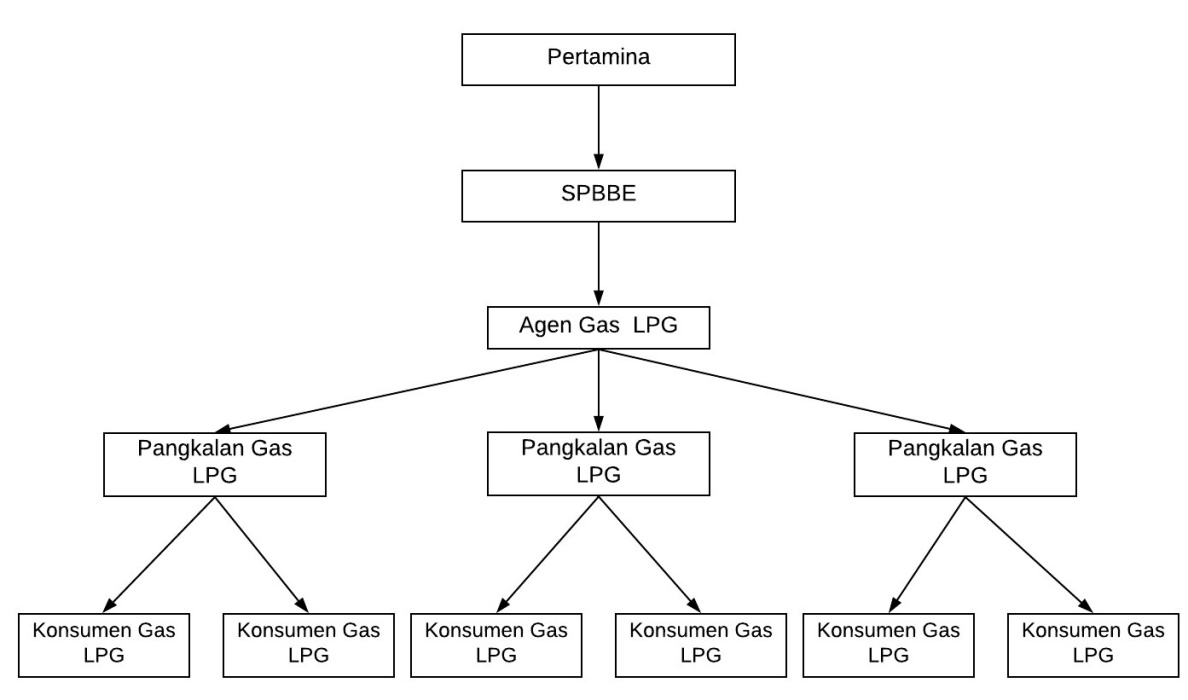
\includegraphics [width = 10cm, height= 10cm]{gambar/struktur-penyaluran}
	\caption{Struktur Penyaluran Gas LPG}
	\label{penyaluran}
\end{figure}


\section{Gas Subsidi LPG 3Kg}
\par Sejak Pemerintah melakukan konversi dari minyak tanah ke gas LPG yang dilakukan pada tahun 2007 menyebabkan kebutuhan untuk tabung gas LPG semakin meningkat dan gas subsidi LPG 3 kg yang ditawarkan pemerintah di awal periode konversi, semakin berkurang. Ini dikarenakan jenis tabung ini dianggap lebih ekonomis di bandingkan dengan tabung gas dan banyak rumah tangga dan industri rumahan kecil yang masih memakai tabung gas jenis ini sebagai alat untuk memasak.
\begin{figure}[H]
	\centering
	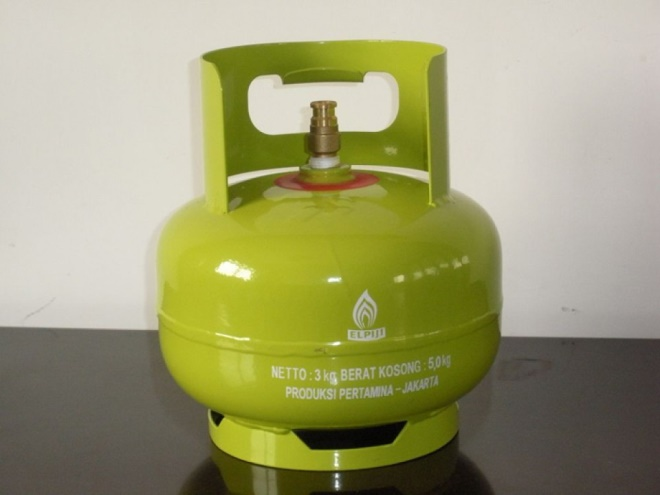
\includegraphics [width = 6cm, height= 8cm]{gambar/tabung-gas}
	\caption{Tabung Gas LPG}
	\label{tabung}
\end{figure}

\par Maka dari itu pertamina selaku distributor telah memberlakukan kebijakan kepada konsumen yang ingin membeli gas subsidi ini harus menunjukkan kartu keluarga (KK) dan Kartu Tanda Penduduk (KTP) sehingga jumlah tabung yang di beli dapat dibatasi berdasarkan KK.

\section{Android}
\par Android merupakan sistem operasi yang dibangun untuk perangkat mobile. Komponen-komponen dari sistem operasi Android ditulis dengan bahasa pemrograman C atau C++, akan tetapi aplikasi pengguna yang digunakan untuk Android ditulis dalam bahasa pemrograman Java \citep{ableson2012android}. Android juga dapat diartikan sebagai sistem operasi perangkat seluler berbasis Linux yang menyediakan run time environment yang disebut dengan \textit{Android Runtime} (ART) yang telah dioptimasi untuk perangkat dengan sistem memori yang kecil. Karena Android merupakan platform open source, maka setiap orang bebas untuk membuat dan mengembangkan suatu aplikasi \citep{supardi2011}.
%\begin{figure}[H]
%	\centering
%	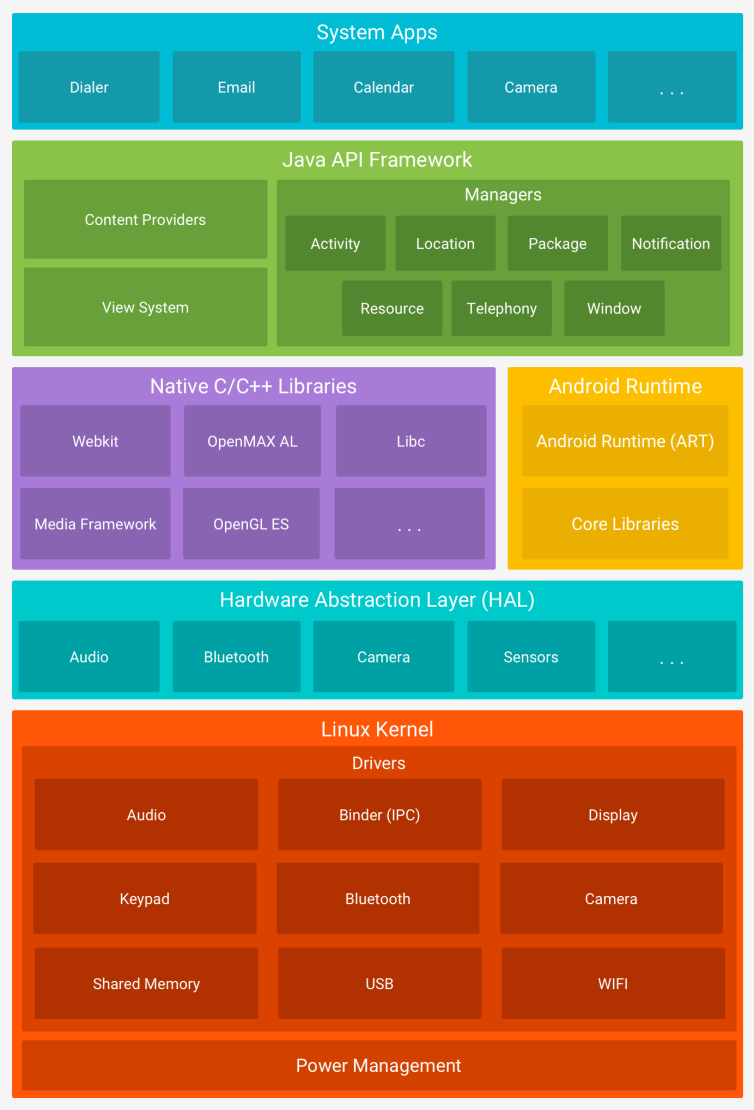
\includegraphics [width = 7cm, height= 6cm]{gambar/android}
%	\caption{Logo Android}
%	\label{android}
%\end{figure}



%-----------------------------------------------------------------------------%
\newpage
\section{Java}
Java pertama kali diluncurkan pada tahun 1995 sebagai bahasa pemrograman umum (\textit{general purpose programming language}) dengan kelebihan dia bisa dijalankan di web browser sebagai applet. Sejak awal, para pembuat Java telah menanamkan visi mereka ke dalam Java untuk membuat piranti-piranti yang ada di rumah (\textit{small embedded customer device}) seperti TV, telepon, radio, dan sebagainya agar dapat berkomunikasi satu sama lain. Karakteristik dari bahasa Java adalah sebagai berikut : \citep{Utama}
\begin{itemize}
	\itemsep0em
	\item Memiliki struktur Syntax yang sederhana
	\item Sangat berorientasi objek (OOP) dengan implementasi yang sangat baik sehingga
	kita bukan hanya belajar bagaimana membuat program yang baik (reusable,
	scalable, dan maintanable) tetapi juga kita belajar bagaimana cara berfikir yang
	baik untuk mengenali struktur masalah yang sedang kita hadapi.
	\item \textit{OpenPlatform}, \textit{Write Once Run Anywhere} (WORA), portabel atau \textit{multi platform}, program yang kita buat dapat dijalankan di Windows, Linux/Unix, Solaris, dan MacIntosh tanpa perlu diubah maupun di kompilasi ulang.
	\item Arsitekturnya yang kokoh dan pemrograman yang aman didukung oleh komunitas
	\textit{Open Source}
	\item Bukan sekedar bahasa tapi juga platform sekaligus arsitektur. Java mempunyai portabilitas yang sangat tinggi.
\end{itemize}

\section{Servlet}
Servlet merupakan salah satu modul perpustakaan yang ditulis dalam bahasa pemrograman Java yang berupa \textit{class} yang digunakan untuk merespon permintaan \textit{client}. Servlet tidak terikat dengan protokol client-server tertentu tetapi paling sering menggunakan protokol HTTP dan kata "Servlet" sering digunakan dalam arti "HTTP Servlet" \citep{zeiger1999servlet}. Penggunaan umum untuk HTTP Servlet meliputi:
\begin{itemize}
	\itemsep0em
	\item Memproses dan / atau menyimpan data yang dikirimkan oleh formulir HTML.
	\item Menyediakan konten dinamis, contohnya mengembalikan hasil kueri basis data ke klien.
	\item Mengelola informasi \textit{state} di dalam protokol \textit{stateless} HTTP.
\end{itemize}
\newpage
\section{Google App Engine}
Google App Engine (GAE) adalah layanan untuk mengembangkan dan hosting aplikasi Web di pusat data Google, yang termasuk ke dalam komputasi awan kategori Platform As Services (PaaS). Google App Engine merupakan layanan yang memaparkan berbagai bagian-bagian dari Infrastruktur skalabilitas tinggi yang di miliki Google. Dengan layanan baru yang disediakan oleh Google ini kita dapat dengan mudah untuk membuat aplikasi handal yang berjalan di bawah beban yang berat dan menggunakan sejumlah data yang besar. Beberapa fitur utama yang dimiliki GAE adalah sebagai berikut: \citep{zahariev2009google}
\begin{itemize}
	\itemsep0em
	\item Layanan web yang dinamis, dengan dukungan penuh untuk teknologi web yang umum.
	\item penyimpanan persisten dengan kueri, pengurutan, dan transaksi.
	\item Penskalaan otomatis dan penyeimbangan beban.
	\item API untuk melakukan autentikasi pengguna dan mengirim email menggunakan Akun Google.
	\item lingkungan pengembangan lokal yang memiliki fitur lengkap yang dapat melakukan simulasi Google App Engine di komputer pengguna.
\end{itemize}

\section{Aplikasi \textit{hybrid} (\textit{Mobile Hybrid App})}
\par Sekarang pasar aplikasi mobile telah menyentuh angka lebih dari 2 juta aplikasi, dengan pengunduhan miliaran kali per tahun dari sejumlah toko aplikasi tertentu (Google Play Store dan Apple App Store). namun, kode yang digunakan untuk satu platform mobile misalnya android yang menggunakan bahasa pemrograman Java tidak dapat digunakan pada platform lain contohnya IOS yang menggunakan bahasa pemrograman Swift. Maka pengembangan dan pemeliharaan aplikasi Native untuk banyak platform menjadi sebuah tantangan besar yang dapat mempengaruhi arah pengembangan aplikasi mobile. Aplikasi \textit{hybrid} dikembangkan dengan menggunakan teknologi web standar misalnya  dan semua permintaan layanan ke API Platform menggunakan oleh API JavaScript \textit{cross-platform}. Dalam konteks ini, kerangka kerja (\textit{framework}) pengembangan aplikasi \textit{hybrid} misalnya Apache Cordova dapat didefinisikan sebagai komponen perangkat lunak yang memungkinkan para pengembang untuk membuat aplikasi \textit{mobile} berbasis web yang dapat berjalan di berbagai platform \citep{malavolta2015hybrid}.
\begin{figure}[H]
	\centering
	\fbox{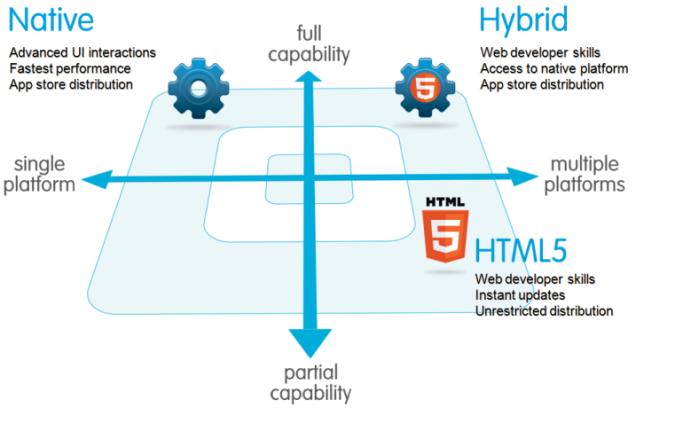
\includegraphics [width = 12cm, height= 8cm]{gambar/hybrid}}
	\caption{Perbandingan Aplikasi Native \& Hybrid}
	\label{android}
\end{figure}

\section{Ionic Framework}

Ionic adalah \textit{framework front-end} yang dikhususkan untuk membangun aplikasi \textit{hybrid} dengan HTML5, CSS dan AngularJS. Ionic menggunakan Node.js SASS, AngularJS sebagai \textit{engine}-nya. Ionic dilengkapi dengan komponen-komponen CSS seperti \textit{button, list, card, form, grids, tabs}, dan masih banyak lagi. Jadi Ionic itu merupakan teknologi web yang bisa digunakan untuk membuat suatu aplikasi \textit{mobile}. Karena \textit{hybrid} maka aplikasi hanya dibuat satu kali tetapi sudah bisa dirilis di lebih dari satu \textit{platform} dengan kata lain \textit{cross-platform} \citep{Ionic}.


\section{Apache Cordova}
\par Seperti yang telah dijelaskan di atas, bahwa Ionic hanya menyediakan \textit{framework Front-end} sedangkan untuk mengubahnya ke dalam \textit{platform} Android dan IOS, Ionic menggunakan Apache Cordova. Apache Cordova adalah kerangka kerja(\textit{framework}) \textit{open-source} yang populer untuk mengembangkan aplikasi \textit{mobile hybrid}. Aplikasi yang dibuat menggunakan Apache Cordova diimplementasikan sebagai halaman web. Halaman web ini dapat menggunakan komponen-komponen teknologi web standar. Komponen kunci untuk memahami cara kerja dari Apache Cordova adalah \textit{WebView}. \textit{WebView} adalah komponen yang disediakan oleh \textit{platform native} untuk memuat dan menjalankan sebuah halaman web. Fitur utama dari Cordova adalah plugin UI(\textit{user interface}) yang memungkinkan kode JavaScript yang berjalan di halaman web untuk dapat berkomunikasi dengan komponen \textit{native} \citep{cheng2017build}.



\section{Angular}
\par Untuk melakukan implementasi logika, Ionic menggunakan teknologi framework javascript bernama Angular yang menawarkan performa dan respon cepat seperti aplikasi \textit{native}. sebelumnya dikenal dengan nama AngularJS, sekarang dikenal dengan nama Angular (tanpa JS dibelakang). Angular yang merupakan versi terkini dari AngularJS tentu masih banyak peminatnya di dunia pemrograman. Angular telah mengalami banyak sekali perubahan dibandingkan pendahulunya AngularJS. Angular kini sudah side by side dengan framework Javascript modern lainnya seperti React, Vue dan lain-lainnya. Secara konsep Angular sudah lumayan matang, dengan mampu mengakomodir component based dan dengan bergabungnya Typescript milik Microsoft dan RxJS milik ReactiveX untuk mendukung kemapanan framework ini. Performa yang dihasilkan oleh Angular kini bisa disejajarkan dengan para kompetitor dikelasnya.


\section{Metode Pengembangan Perangkat Lunak}
Pengembangan perangkat lunak dapat diartikan sebagai proses-proses yang dilakukan untuk memgembangkan suatu perangkat lunak yang baru atau memperbaiki perangkat lunak yang telah ada. Agar proses-proses tersebut berjalan lebih cepat, tepat, dan juga hasilnya mudah di kembangkan dan dipelihara, maka pengembangan perangkat lunak memerlukan suatu metodologi khusus. Metodologi Pengembangan Perangkat Lunak merupakan suatu proses pengelolaan kumpulan metode dan konvensi notasi yang telah didefinisikan untuk mengembangkan perangkat lunak. Metode pengembangan perangkat lunak secara prinsip bertujuan untuk membantu menghasilkan perangkat lunak yang berkualitas \citep{jauhari}. Komponen metodologi pengembangan perangkat lunak dapat dibagi dalam tiga unit, yaitu \citep{pressman2005software}:
\begin{enumerate}
	\item Metode, yaitu suatu cara atau teknik pendekatan yang sistematik yang dipergunakan untuk mengembangkan perangkat lunak. Metode ini mencakup : Perencanaan proyek dan  perkiraan, analisis keperluan sistem dan perangkat lunak, perancangan struktur data, arsitektur program, prosedur algoritma, Coding, uji coba dan pemeliharaan.
	\item Alat bantu (\textit{Tools}), yaitu alat-alat (manual atau otomatis) yang mendukung pengembangan  perangkat lunak. Terdapat 2 alat Bantu yang dapat digunakan yaitu : alat Bantu manual dan alat Bantu otomatis.
	\item Prosedur, yang dipergunakan untuk mendefinisikan urut-urutan pekerjaan (siklus) dari metode dan alat bantu tersebut.
\end{enumerate}

\section{Scrum}
Scrum adalah bagian dari metode Agile yang dirancang untuk menambah fokus, kejelasan dan transparansi pada perencanaan dan implementasi proyek. Agile sendiri merupakan pendekatan pengembangan perangkat lunak yang mengutamakan pada kesiapan untuk melakukan perubahan pada tahap pengembangan perangkat lunak \citep{raharjana2017pengembangan}. Scrum digunakan dalam perusahaan perangkat lunak kecil, menengah dan besar di seluruh dunia. Kelebihan dari metode pengembangan perangkat lunak menggunakan Scrum adalah sebagai berikut: 
\begin{itemize}
	\itemsep0em
	\item Meningkatkan kecepatan proses pengembangan.
	\item Menyamakan tujuan individu dan perusahaan.
	\item Menciptakan budaya yang didorong oleh kinerja.
	\item Mendukung pembuatan nilai pemegang saham.
	\item Tercapainya komunikasi kinerja yang stabil dan konsisten di semua tingkatan.
	\item Meningkatkan pengembangan individu dan kualitas hidup
\end{itemize}

\par Komponen utama dari Scrum adalah tim Scrum dan peran, acara, dan artefak yang terkait dengannya. tim Scrum terdiri dari 3 peran yaitu \textit{Product Owner}, \textit{Scrum Master} dan \textit{Development Team}. \textit{Product Owner} adalah satu-satunya orang yang bertanggung jawab dalam pengelolaan Product Backlog. \textit{Development Team} dibentuk dan diberikan wewenang oleh organisasi untuk menyusun dan mengelola pekerjaan mereka sendiri. \textit{Scrum Master} bertanggung jawab untuk mengenalkan dan menyokong penggunaan Scrum sebagaimana dijelaskan di dalam Panduan Scrum ini. \textit{Scrum Master} melakukan ini dengan membantu orang-orang agar dapat memahami teori, praktik-praktik, aturan-aturan dan tata nilai Scrum. Scrum memiliki beberapa artefak-artefak atau dokumen yang merepresentasikan pekerjaan atau nilai bisnis guna terciptanya transparansi dan kesempatan untuk menginspeksi dan mengadaptasi. artefak-artefak terdiri dari Product Backlog dan Sprint Backlog.

\par \textit{Product Backlog} adalah daftar terurut dari seluruh fitur, fungsi, kebutuhan, peningkatan, dan perbaikan yang perlu diberlakukan terhadap produk pada rilis mendatang. Product Backlog item memiliki atribut deskripsi, urutan, estimasi dan nilai bisnis. Sedangkan, \textit{Sprint Backlog} adalah daftar item pada \textit{Product Backlog} yang terpilih untuk Sprint ditambah perencanaan untuk menghantarkan \textit{Increment} dan mencapai Sprint Goal. 

\par Scrum memiliki beberapa acara yang wajib dilakukan oleh seluruh anggota tim Scrum yaitu \textit{Sprint, Sprint Planning, Daily Scrum, Sprint Review, Sprint Retrospective}. Bagian terpenting dari Scrum adalah \textit{Sprint}, yaitu sebuah batasan waktu dengan durasi satu bulan atau kurang, dimana terdapat proses pembuatan \textit{Increment} yang dianggap “Selesai”. \textit{Increment} sendiri merupakan kumpulan item pada \textit{Product Backlog} yang diselesaikan dalam \textit{Sprint} dan total nilai bisnis \textit{Increment} dari seluruh \textit{Sprint} yang lalu.

\par \textit{Sprint Planning} adalah proses untuk merencanakan pekerjaan yang akan dikerjakan di \textit{Sprint}. Perencanaan ini dilakukan secara kolaboratif oleh seluruh anggota tim Scrum. \textit{Sprint Planning} memiliki batasan waktu maksimal delapan jam untuk Sprint yang berdurasi satu
bulan. \textit{Daily Scrum} adalah acara untuk \textit{Development Team} yang memiliki batasan waktu 15 menit. Dilakukan setiap hari selama Sprint berlangsung. \textit{Development Team} akan membuat rencana kerja untuk 24 jam ke depan. Acara ini mengoptimalkan kolaborasi dan performa dari tim dengan melakukan inspeksi pada pekerjaan yang dilakukan semenjak Daily Scrum sebelumnya.

\par \textit{Sprint Review} diselenggarakan di akhir setiap \textit{Sprint} untuk menginspeksi \textit{Increment} dan mengadaptasi \textit{Product Backlog} bila diperlukan. Pada saat \textit{Sprint Review}, tim Scrum dan pemegang kepentingan berkolaborasi untuk meninjau apa yang sudah   diselesaikan di Sprint. \textit{Sprint Retrospective} diselenggarakan setelah \textit{Sprint Review} dan sebelum \textit{Sprint Planning} berikutnya. Acara ini diselenggarakan paling lama tiga jam untuk Sprint yang berdurasi satu bulan. Untuk \textit{Sprint} yang lebih singkat, durasi acara ini biasanya lebih singka \citep{sutherlandpanduan}. Tujuan dari \textit{Sprint Retrospective} adalah:
\begin{itemize}
	\itemsep0em
	\item Melakukan inspeksi bagaimana jalannya Sprint terakhir yang terkait dengan orang-orang, hubungan antar mereka, proses, dan alat-alat yang digunakan.
	\item Melakukan identifikasi dan mengurutkan hal utama yang berjalan dengan baik dan peningkatan yang berpotensi untuk dilakukan.
	\item Membuat perencanaan untuk implementasi peningkatan cara kerja tim Scrum.
\end{itemize}
 

\section {\textit{Test Plan}}
\par Test Plan merupakan dokumen yang berisi definisi tujuan dan sasaran pengujian dalam lingkup iterasi (atau proyek), item-item yang menjadi target pengujian, pendekatan yang akan diambil, sumber daya yang dibutuhkan dan point untuk diproduksi. Dengan kata lain test plan dapat disebut sebagai perencanaan atau skenario untuk melakukan testing yang akan dilakukan baik oleh expert atau user umum. 
\par Tujuan umum membuat test plan secara umum adalah untuk memudahkan developer untuk melakukan testing agar testing yang dilakukan menjadi jelas sehingga hasilnya lebih berguna dan efisien. Tentunya dalam proses pembuatan test plan ini memerlukan beberapa langkah seperti berikut : \citep{software2008ieee}
\begin{itemize}
	\item {Melakukan Analisa Produk}
	\newline Pada tahap ini kita harus meneliti seluruh bagian dari produk dan  meninjau dokumentasi dari produk. meninjau dokumentasi produk akan membantu memahami semua fitur-fitur dalam produk tersebut
	
	\item {Mengembangkan Strategi Pengujian}
	\newline Strategi pengujian adalah langkah yang penting saat membuat \textit{test plan}. berikut tahapan membuat strategi pengujian :
	\begin{itemize}
		\itemsep0em
		\item Mendefinisikan cakupan dari pengujian
		\item Mengidentifikasi Jenis Pengujian
		\item Dokumentasikan Resiko dan Masalah
		\item Menyiapkan Logistik Pengujian
	\end{itemize}
	
	\item {Mendefinisikan Objektif Pengujian}
	\newline Objektif Pengujian adalah keseluruhan tujuan dan pencapaian dari pelaksanaan pengujian. Tujuan pengujian ini adalah menemukan sebanyak mungkin cacat pada produk dan memastikan bahwa produk yang diuji bebas dari bug sebelum dirilis.
	
	\item Mendefinisikan Kriteria Pengujian
	\newline kriteria pengujian merupakan standar atau aturan yang prosedur atau penilaian pengujian dapat didasarkan. Ada 2 jenis kriteria pengujian yaitu sebagai berikut :
	\begin{itemize}
		\itemsep0em
		\item \textit{Suspension Criteria} : apabila kriteria ini terpenuhi maka siklus pengujian akan ditunda sampai permasalahan telah selesai
		\item \textit{Exit Criteria} : target persentase dari hasil pengujian yang dibutuhkan sebelum dilanjutkan ke tahap pengembangan selanjutnya
	\end{itemize}

	\item {Merencanakan Sumber Daya}
	\newline Rencana sumber daya merupakan ringkasan rinci dari semua jenis sumber daya yang dibutuhkan untuk menyelesaikan tugas proyek. Sumber daya dapat berupa manusia, peralatan dan material yang dibutuhkan untuk menyelesaikan proyek.
	
	\newpage
	\item Merencanakan Lingkungan Pengujian
	\newline Lingkungan pengujian adalah pengaturan perangkat lunak dan perangkat keras yang akan digunakan tim pengujian untuk melakukan uji coba. Lingkungan pengujian terdiri dari lingkungan bisnis dan pengguna yang nyata, serta lingkungan fisik, seperti server, lingkungan yang menjalankan ujung depan.
	
	\item {Melakukan Penjadwalan dan Estimasi}
	 \newline Dengan membuat jadwal yang padat dalam Perencanaan Pengujian, Manajer Pengujian dapat menggunakannya sebagai alat untuk memantau kemajuan dari proyek, mengendalikan pembengkakan biaya.
	 
	 \item {\textit{Test Deliverables}}
	 \newline \textit{Test Deliverables} adalah daftar semua dokumen, alat, dan komponen lain yang harus dikembangkan dan dipelihara untuk mendukung upaya pengujian.
	
\end{itemize}

\section {\textit{Usability Testing}}
\par \textit{Usability Testing} atau tes produk merupakan metode riset untuk mengembangkan dan menyempurnakan produk baru maupun yang telah ada. Inti dari riset ini adalah mendudukkan pengguna/pelanggan di pusat, lalu mengambil pelajaran dari sana. maka dalam test ini, mutlak adanya pengamatan secara langsung. Dengan mendokumentasikan pengalaman aktual dari para calon pengguna aplikasi/produk diharapkan akan menangkap kekuatan dan kelemahan dari setiap aspek yang ada pada aplikasi itu sendiri \citep{nielsen2012}.

\section {\textit{Unit Testing}}
\textit{Unit Testing} adalah metode untuk melakukan verifikasi pada perangkat lunak di mana programmer menguji suatu unit program layak untuk dipakai. Unit testing ini fokus pada verifikasi pada unit yang terkecil pada desain perangkat lunak (komponen atau modul perangkat lunak). Karena dalam sebuah perangkat lunak banyak memiliki unit-unit kecil maka untuk mengujinya biasanya dibuat program kecil atau main program) untuk menguji unit-unit perangkat lunak. Unit-unit kecil ini dapat berupa prosedur atau fungsi, sekumpulan prosedur atau fungsi yang ada dalam satu file jika dalam pemrograman terstruktur, atau kelas, bisa juga kumpulan kelas dalam satu package. \citep{rosa2013rekayasa}

%-----------------------------------------------------------------------------%

% Baris ini digunakan untuk membantu dalam melakukan sitasi
% Karena diapit dengan comment, maka baris ini akan diabaikan
% oleh compiler LaTeX.
\begin{comment}
\bibliography{daftar-pustaka}
\end{comment}


%-------------------------------------------------------------------------------
%                            BAB III
%               		METODOLOGI PENELITIAN
%-------------------------------------------------------------------------------

\chapter{METODOLOGI PENELITIAN}

\section{Tempat dan Waktu Penelitian}
\setlength\parindent{30pt} Penelitian ini dilakukan di Jurusan Informatika, Fakultas Matematika dan Ilmu Pengetahuan Alam, Universitas Syiah Kuala Banda Aceh. Waktu yang diperlukan untuk melakukan penelitian ini kurang lebih selama lima bulan, yang dimulai dari bulan Juni 2018 sampai bulan Desember 2018.

% Please remember to add \use{multirow} to your document preamble in order to suppor multirow cells
\begin{table}[H]
	\center
	\caption{Jadwal Penelitian.}
	\label{jadwal}
	\begin{tabular}{|c|l|l|l|l|l|l|l|}
		\hline
		\multirow{2}{*}{No} & \multirow{2}{*}{Keterangan} 	& \multicolumn{6}{c|}{Bulan}           																										\\ \cline{3-8} 
							&                           	& Jul				& Agt  			& Sep			& Okt			& Nov			& Des 					\\ \hline       
		1                   & Studi literatur           	&\cellcolor{gray}	&\cellcolor{gray}	&                   &                   &                   &                       	\\ \hline
		2                   & Penulisan Proposal           	&                   &\cellcolor{gray}	&\cellcolor{gray}	&                   &                   &                        	\\ \hline
		3                   & Pengembangan Aplikasi         &                   &                   & \cellcolor{gray}  & \cellcolor{gray} 	& \cellcolor{gray}  &                            \\ \hline
		4                   & Evaluasi Sistem               &                   &                   &           		&             		&\cellcolor{gray}	&  \cellcolor{gray}    \\ \hline
		5                   & Penulisan Laporan Akhir       &                   &                   &                   &        			&      				& \cellcolor{gray}     \\ \hline
	\end{tabular}
\end{table}

\section{Alat dan Bahan}
Alat yang digunakan pada penelitian ini adalah sebagai berikut :

\begin{enumerate}[a.]
\item Perangkat Keras (\textit{Hardware})
	\begin{itemize}
		\item 1 unit Laptop HP Intel(R) Core(TM) i7 6700HQ
		\item RAM 8 GB DDR3
		\item Harddisk 1 TB
		\item 1 unit Android Samsung S7
	\end{itemize}

\item Perangkat Lunak (\textit{Software})
	\begin{itemize}
		\item Visual Studio Code
		\item Cordova 7.0.0
		\item Ionic Framework 3
		\item SDK Android 27.0.1
	\end{itemize}
\end{enumerate}

\section{Metode Penelitian}
Skema dari alur tahapan penelitian dapat dilihat pada Gambar \ref{alur}
\vspace{-0.4cm}
\begin{figure}[H]
	\center
	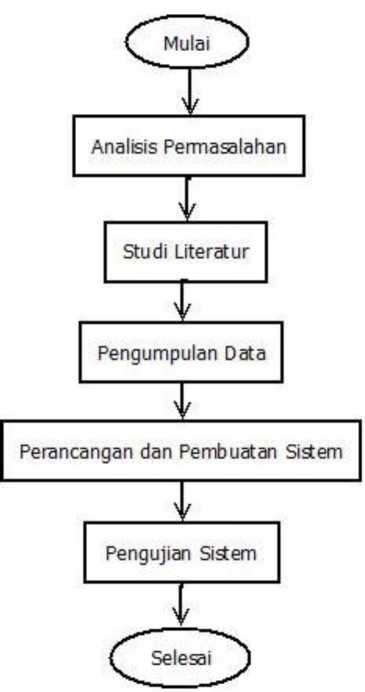
\includegraphics [width = 6cm, height= 10cm]{gambar/alur2}
	\caption{Diagram Alir Penelitian}
	\label{alur}
\end{figure}

\subsection{Analisis Permasalahan}
Aplikasi ini merupakan aplikasi berbasis mobile yang berguna untuk membantu pangkalan gas LPG Subsidi 3 Kg dalam melakukan pelaporan penyaluran tabung gas subsidi. Aplikasi ini juga membantu agen gas LPG selaku distributor dan pengawasan dari pangkalan gas untuk melakukan rekap laporan penyaluran tabung gas 3 Kg. Aplikasi ini melakukan pelaporan penyaluran tabung gas subsidi dengan menggunakan NIK(Nomor Induk Kependudukan) dan no telepon sebagai data acuan yang valid. Setelah itu data tersebut langsung di kirim langsung ke agen gas LPG bersangkutan. Adapun fitur-fitur yang terdapat pada aplikasi ini adalah sebagai berikut
\begin{itemize}
		\itemsep0em
		\item Masuk ke dalam aplikasi.
		\item Melihat jadwal pasokan tabung.
		\item Mencatat penjualan tabung gas menggunakan NIK sebagai acuan.
		\item Mencetak kartu kendali untuk konsumen.
		\item Mengubah profile biodata user.
\end{itemize}

\subsection{Studi Literatur}
Studi literatur dilakukan dengan mencari jurnal baik nasional maupun internasional, buku, serta beberapa literatur elektronik yang diunduh dari internet yang terkait dengan penelitian ini. Studi literatur juga diperoleh dari penelitian sebelumnya yang berkaitan dengan penelitian. Studi literatur digunakan sebagai bahan referensi selama proses penelitian.

\subsection{Pengumpulan Data}
Data yang digunakan dalam penelitian ini adalah data penyaluran tabung dan format pelaporan yang dipakai. Data tersebut didapatkan dari agen dan pangkalan yang menjadi objek penelitian.

\subsection{Perancangan dan Pembuatan Sistem}
Dalam merancang aplikasi ini, digunakan metode pengembangan perangkat lunak yaitu eXtreme Programming (XP). Metode XP fleksibel terhadap perubahan-perubahan sehingga cocok digunakan pada aplikasi ini. Berikut merupakan tahapan perancangan sistem yang akan dilakukan:

\begin{enumerate}[1.]
	\item \emph {Planning}
	
	Pada tahap ini dikumpulkan kebutuhan awal user atau dalam XP dikenal dengan istilah \emph {user requirement}. Hal ini dibutuhkan agar kebutuhan \emph {output} sistem, dan fitur utama dari aplikasi yang dikembangkan terdefinisikan dengan jelas. Selanjutnya dilakukan analisa kebutuhan awal terhadap aplikasi:
	
	\begin{enumerate}[a.]
		\item \textit{User Story}
		User story adalah deskripsi singkat dan sederhana mengenai fitur atau fungsi dari software, dilihat dari sudut pandang pengguna. Berikut ini merupakan user story dari kasus penelitian ini.
		\begin{itemize}
			\item \textbf{ID: 01}
			\par Sebagai pangkalan, saya ingin mencatat penjualan tabung ke dalam laporan logbook.
			\item \textbf{ID: 02}
			\par Sebagai pangkalan, saya ingin mengetahui jadwal pasokan/penerimaan tabung gas
			\item \textbf{ID: 03}
			\par Sebagai pangkalan, saya ingin melakukan login ke dalam aplikasi
			\item \textbf{ID: 04}
			\par Sebagai pangkalan, saya ingin mendaftarkan konsumen baru.
			\item \textbf{ID: 05}
			\par Sebagai agen, saya ingin melakukan rekap laporan dari masing-masing pangkalan milik saya.
			\item \textbf{ID: 06}
			\par Sebagai agen, saya ingin menetapkan kuota tabung per bulan untuk masing-masing pangkalan.
			\item \textbf{ID: 07}
			\par Sebagai pangkalan, saya ingin mencetak kartu kendali konsumen untuk pangkalan kecil yang belum memiliki mesin cetak.
		\end{itemize}
		Penggunaan nomor unik ID pada user story dilakukan untuk memudahkan pengelolaan \textit{user story} sekaligus membedakan satu \textit{user story} dengan yang lainnya.
		
		\item Kebutuhan Fungsional
		\newline Kebutuhan fungsional, dapat dimodelkan pada use case diagram. Use case diagram adalah diagram yang memodelkan perilaku dari sistem. Di dalam use case diagram terdapat sekumpulan use case, aktor dan hubungan antara use case dan aktor. Use case diagram dapat dilihat pada \ref{usecase} di bawah ini.
		
		\vspace{-0.4cm}
		\begin{figure}[H]
			\center
			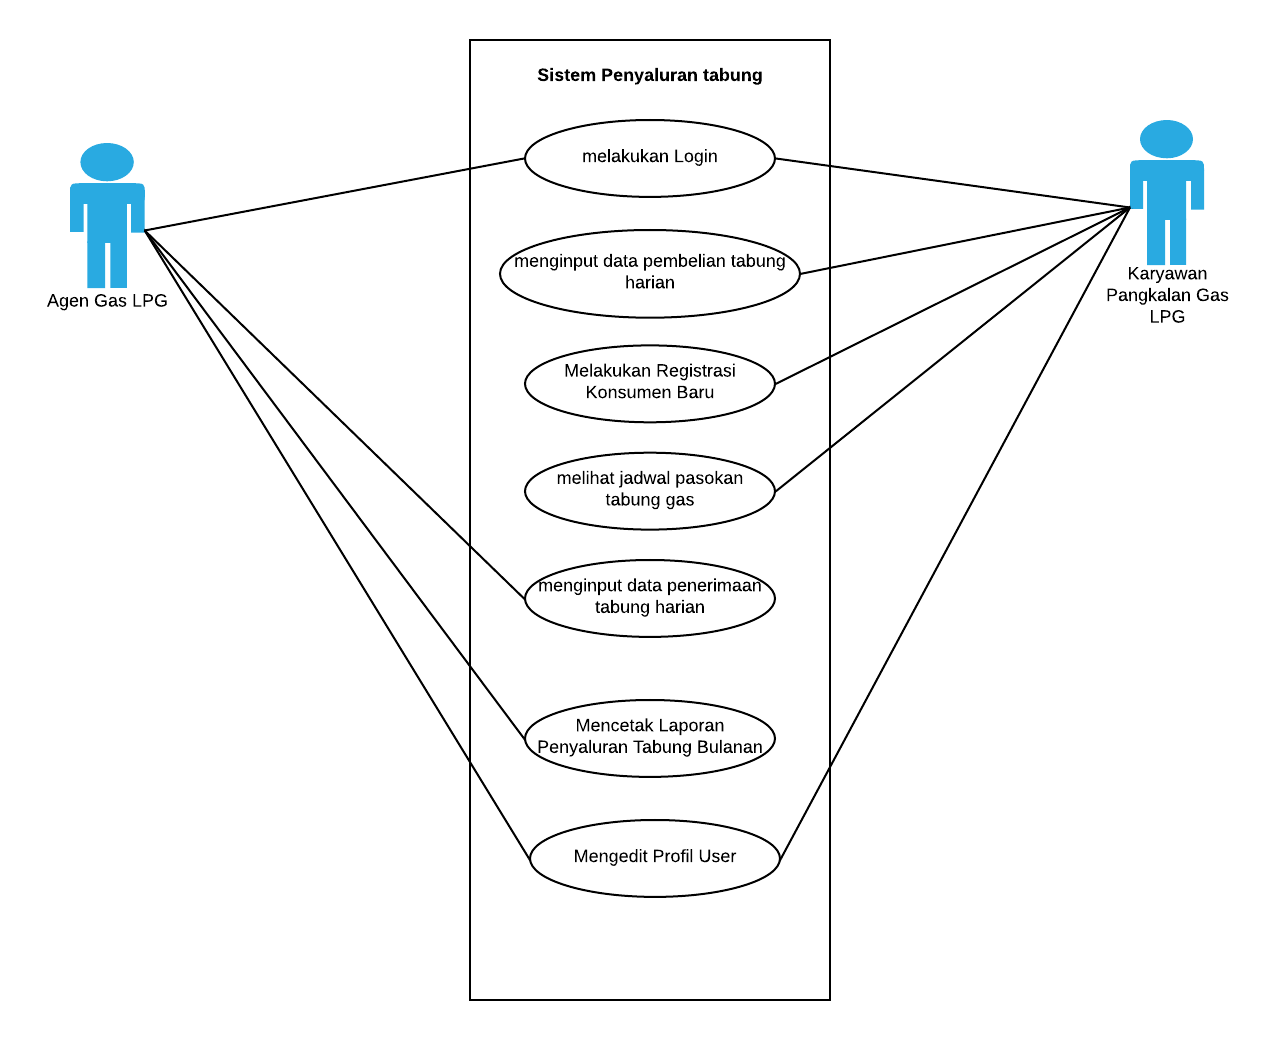
\includegraphics [width = 12cm, height= 11cm]{gambar/use-case}
			\caption{Diagram Use-Case}
			\label{usecase}
		\end{figure}
		
		\newpage
		\item Kebutuhan Non Fungsional
		\newline Kebutuhan non-fungsional adalah batasan dalam layanan atau fungsi yang ditawarkan sistem. Dalam penelitian ini, kebutuhan non-fungsional yang digunakan ada dua macam, seperti pada Tabel 3.2.
		
		\vspace{-0.4cm}
		\begin{table}[H]
			\centering
			\caption{Kebutuhan Non-Fungsional}
			\label{kebutuhan}
			\begin{tabular}{|l|p{5cm} |}
				\hline
				Jenis Kebutuhan & Deskripsi \\ 
				\hline 
				\textit{Usability} & Sistem yang dibuat harus dapat dipelajari dan digunakan dengan mudah oleh pengguna. Kemudahan-kemudahan tersebut diantaranya kemudahan dalam hal penggunaan sistem. \\ 
				\hline 
				\textit{Compatibility} & Sistem dapat diakses melalui beberapa versi sistem operasi Android. \\ 
				\hline 
			\end{tabular} 
		\end{table}
		
		
	\end{enumerate}

	\item \textit{Design}
	
	Tahap ini fokus pada desain pembuatan program perangkat lunak termasuk struktur data, arsitektur perangkat lunak, representasi antarmuka dan prosedur pengkodean. Representasi perangkat lunak yang dikembangkan digambarkan dalam sebuah pemodelan. Tahapan perancangan dilakukan berdasarkan dari hasil analisis kebutuhan perangkat lunak pada tahap sebelumnya. Tahapan desain ini meliputi perancangan Unified Modelling Languange (UML), perancangan database dan perancangan desain tampilan (user interface).
	
	\item \textit{Coding}
	
	Pada tahapan ini, dilakukan implementasi terhadap desain yang telah dibuat sebelumnya ke dalam bentuk program. Penulisan kode program dalam penelitian ini menggunakan bahasa pemrograman Typescript untuk aplikasi berbasis Android dan bahasa pemrograman PHP untuk web service yang akan digunakan oleh aplikasi untuk berkomunikasi dengan database.
	
	\newpage
	 \item \textit{Testing}
	
	Tahapan \textit{testing} yang dilakukan diantaranya adalah sebagai berikut:
	\begin{enumerate}[a.]
			\itemsep0em
			\item \textit{Usability}
			\newline Pengujian \textit{usability} digunakan untuk mengetahui seberapa mudah aplikasi dapat dijalankan oleh pengguna. Teknik pengujian \textit{usability} yang digunakan adalah dengan memberikan kuesioner kepada setiap kelompok user yaitu agen gas LPG dan pangkalan gas LPG. Jenis pertanyaan yang ada pada kuesioner mengacu pada kuesioner SUS (\textit{System Usability Scale}). Dalam pengujian \textit{usability} ini, melibatkan sekitar 8 pengguna yang berbeda.
			\item \textit{Unit Testing}
			\newline Unit testing fokus pada verifikasi pada unit yang terkecil pada desain perangkat lunak (komponen atau modul perangkat lunak). Karena dalam sebuah perangkat lunak banyak memiliki unit-unit kecil maka untuk mengujinya biasanya dibuat program kecil atau main program) untuk menguji unit-unit perangkat lunak.
		
	\end{enumerate}
	
	
\end{enumerate}


% Baris ini digunakan untuk membantu dalam melakukan sitasi
% Karena diapit dengan comment, maka baris ini akan diabaikan
% oleh compiler LaTeX.
\begin{comment}
\bibliography{daftar-pustaka}
\end{comment}


%-------------------------------------------------------------------------------
%                            BAB IV
%               		HASIL DAN PEMBAHASAN
%-------------------------------------------------------------------------------

\chapter{HASIL DAN PEMBAHASAN}
	\section{Analisis Kebutuhan}
	
	Hasil dari analisis kebutuhan yang telah dilakukan adalah mendapatkan persona, storyboard dan use case diagram untuk masing-masing pengguna.
	
	\subsection{Kelompok Pengguna}
	Kelompok pengguna dari aplikasi ini telah dapat diidentifikasikan pada tahap analisis kebutuhan pada sistem. terdapat 2 kelompok pengguna yang menggunakan aplikasi ini:
		 \begin{enumerate}[1.]
		 	\item Agen
		 		\newline Pengguna yang menggunakan aplikasi berbasis web untuk mengelola rencana penerimaan pasokan tabung ke pangkalan, melakukan rekapitulasi data penyaluran tabung pada pangkalan.
		 	\item Pangkalan
		 		\newline Pengguna yang menggunakan aplikasi berbasis android untuk melakukan pencatatan penjualan tabung per hari, mendaftarkan pelanggan baru, melakukan verifikasi pada penerimaan pasokan tabung.
		 \end{enumerate}
	 
	 Persona untuk masing-masing kelompok pengguna dapat dilihat pada lampiran 1
	
	\subsection{Storyboard}
	Dengan menggunakan \textit{Storyboard} kita dapat memetakan secara visual kegiatan pengguna sebelum dan sesudah menggunakan aplikasi. Berdasarkan hasil pengamatan dan analisis kebutuhan dapat digambarkan \textit{Storyboard} seperti berikut:
	
	\vspace{-0.4cm}
	\begin{figure}[H]
		\center
		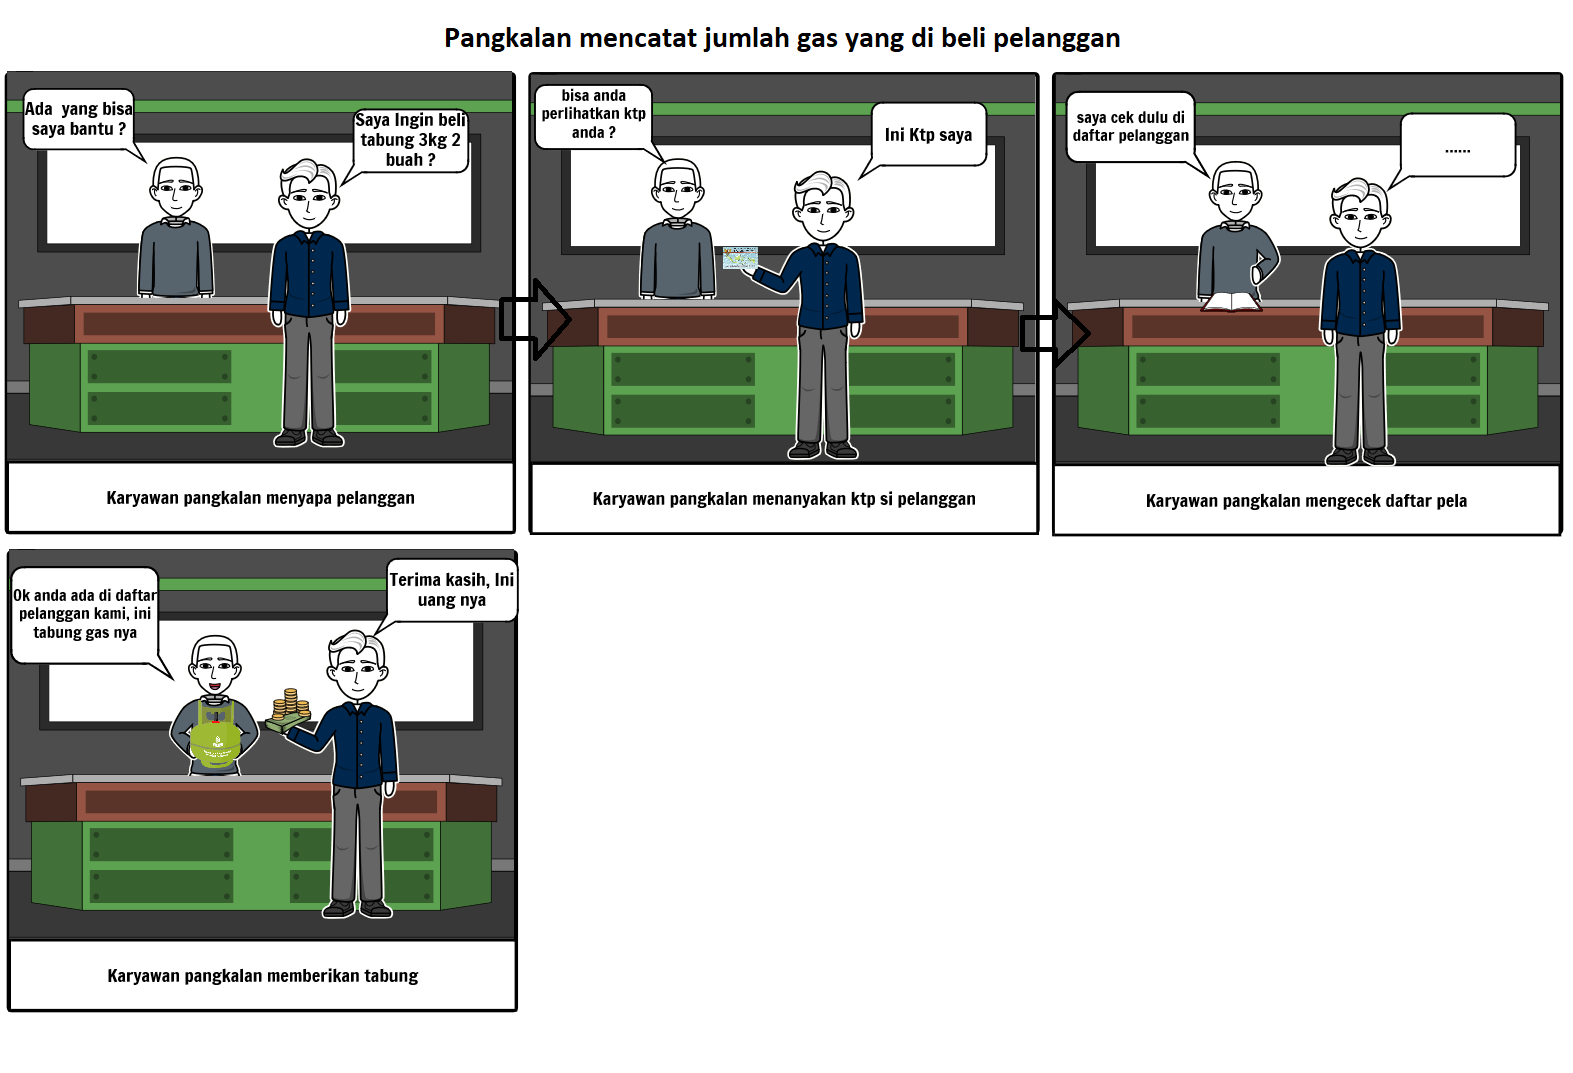
\includegraphics [width = 14cm]{gambar/storyboard/storyboard-1-(old)}
		\caption{Kegiatan Sebelum Menggunakan Aplikasi}
		\label{storyboardOld1}
	\end{figure}
	
	\begin{figure}[H]
		\center
		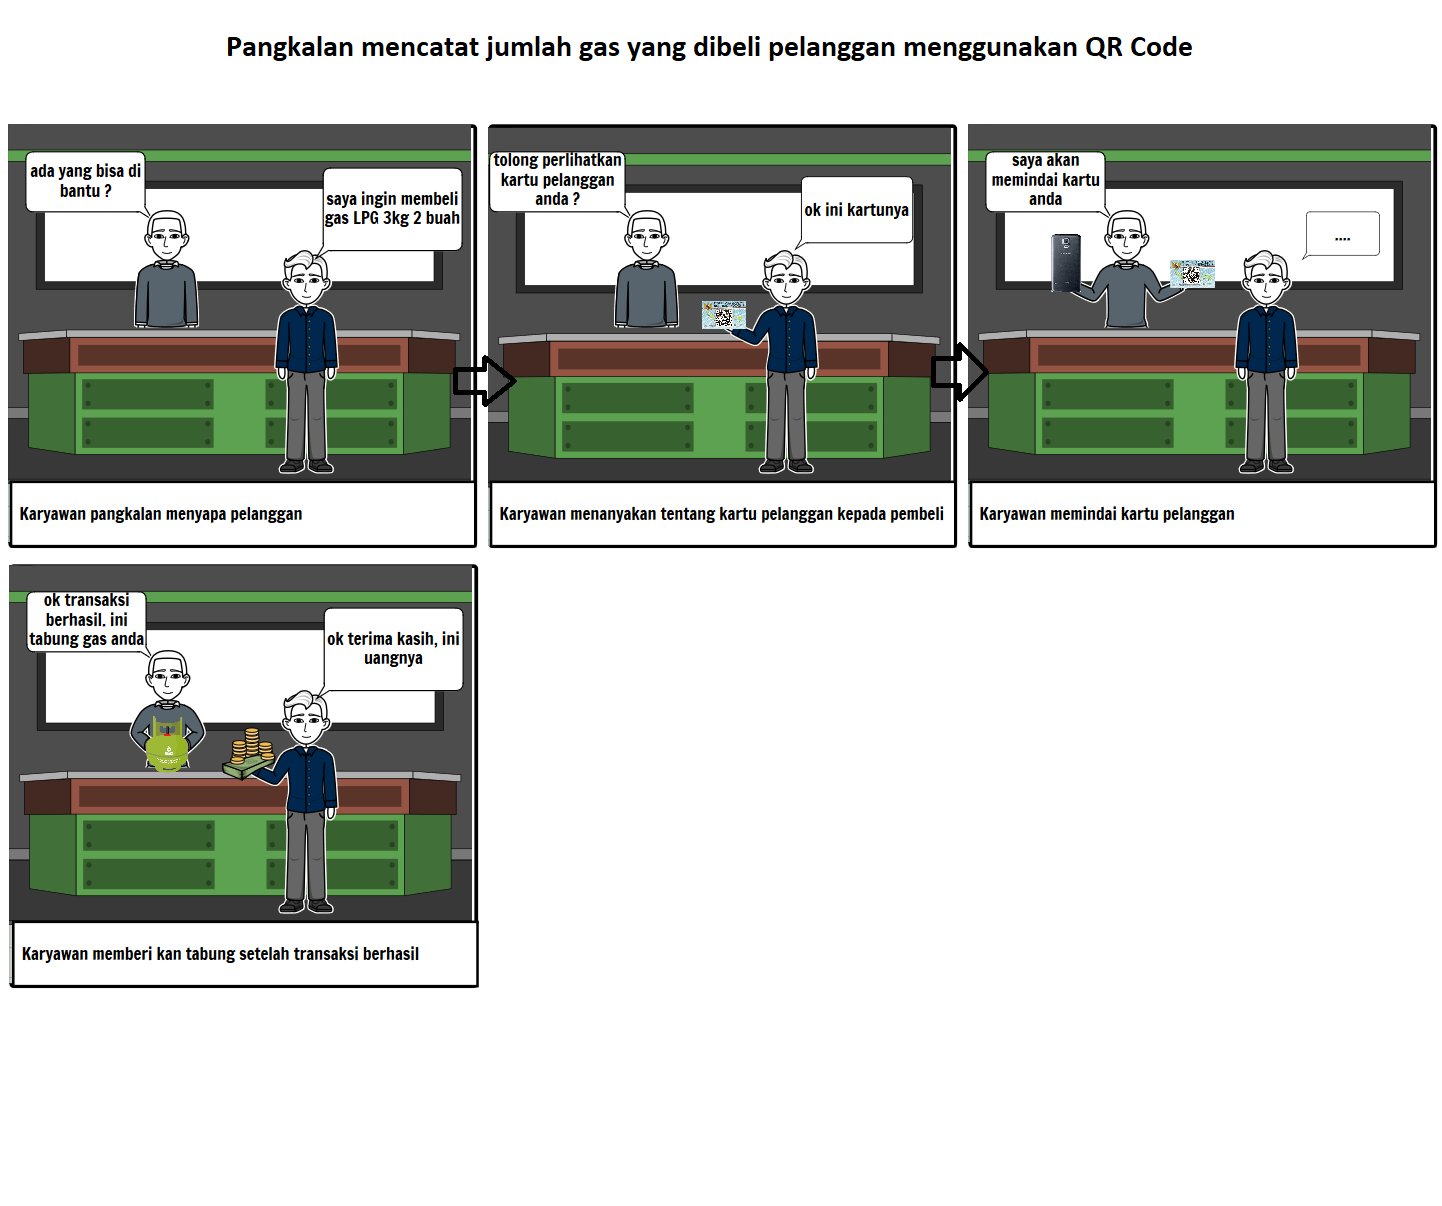
\includegraphics [width = 14cm]{gambar/storyboard/storyboard-1-(new)}
		\caption{Kegiatan Sesudah Menggunakan Aplikasi}
		\label{storyboardNew1}
	\end{figure}
	
	
	
	\subsection{\textit{Value Proposition Canvas }(VPC)}
	Dengan Menggunakan \textit{Value Proposition Canvas} (VPC) ini, kita dapat menguji apakah desain aplikasi dan fitur-fiturnya telah memenuhi kebutuhan dari pengguna aplikasi. Dari hasil pengamatan yang telah dilakukan maka dapat digambarkan VPC sebagai berikut:
	
		\vspace{-0.4cm}
	\begin{figure}[H]
		\center
		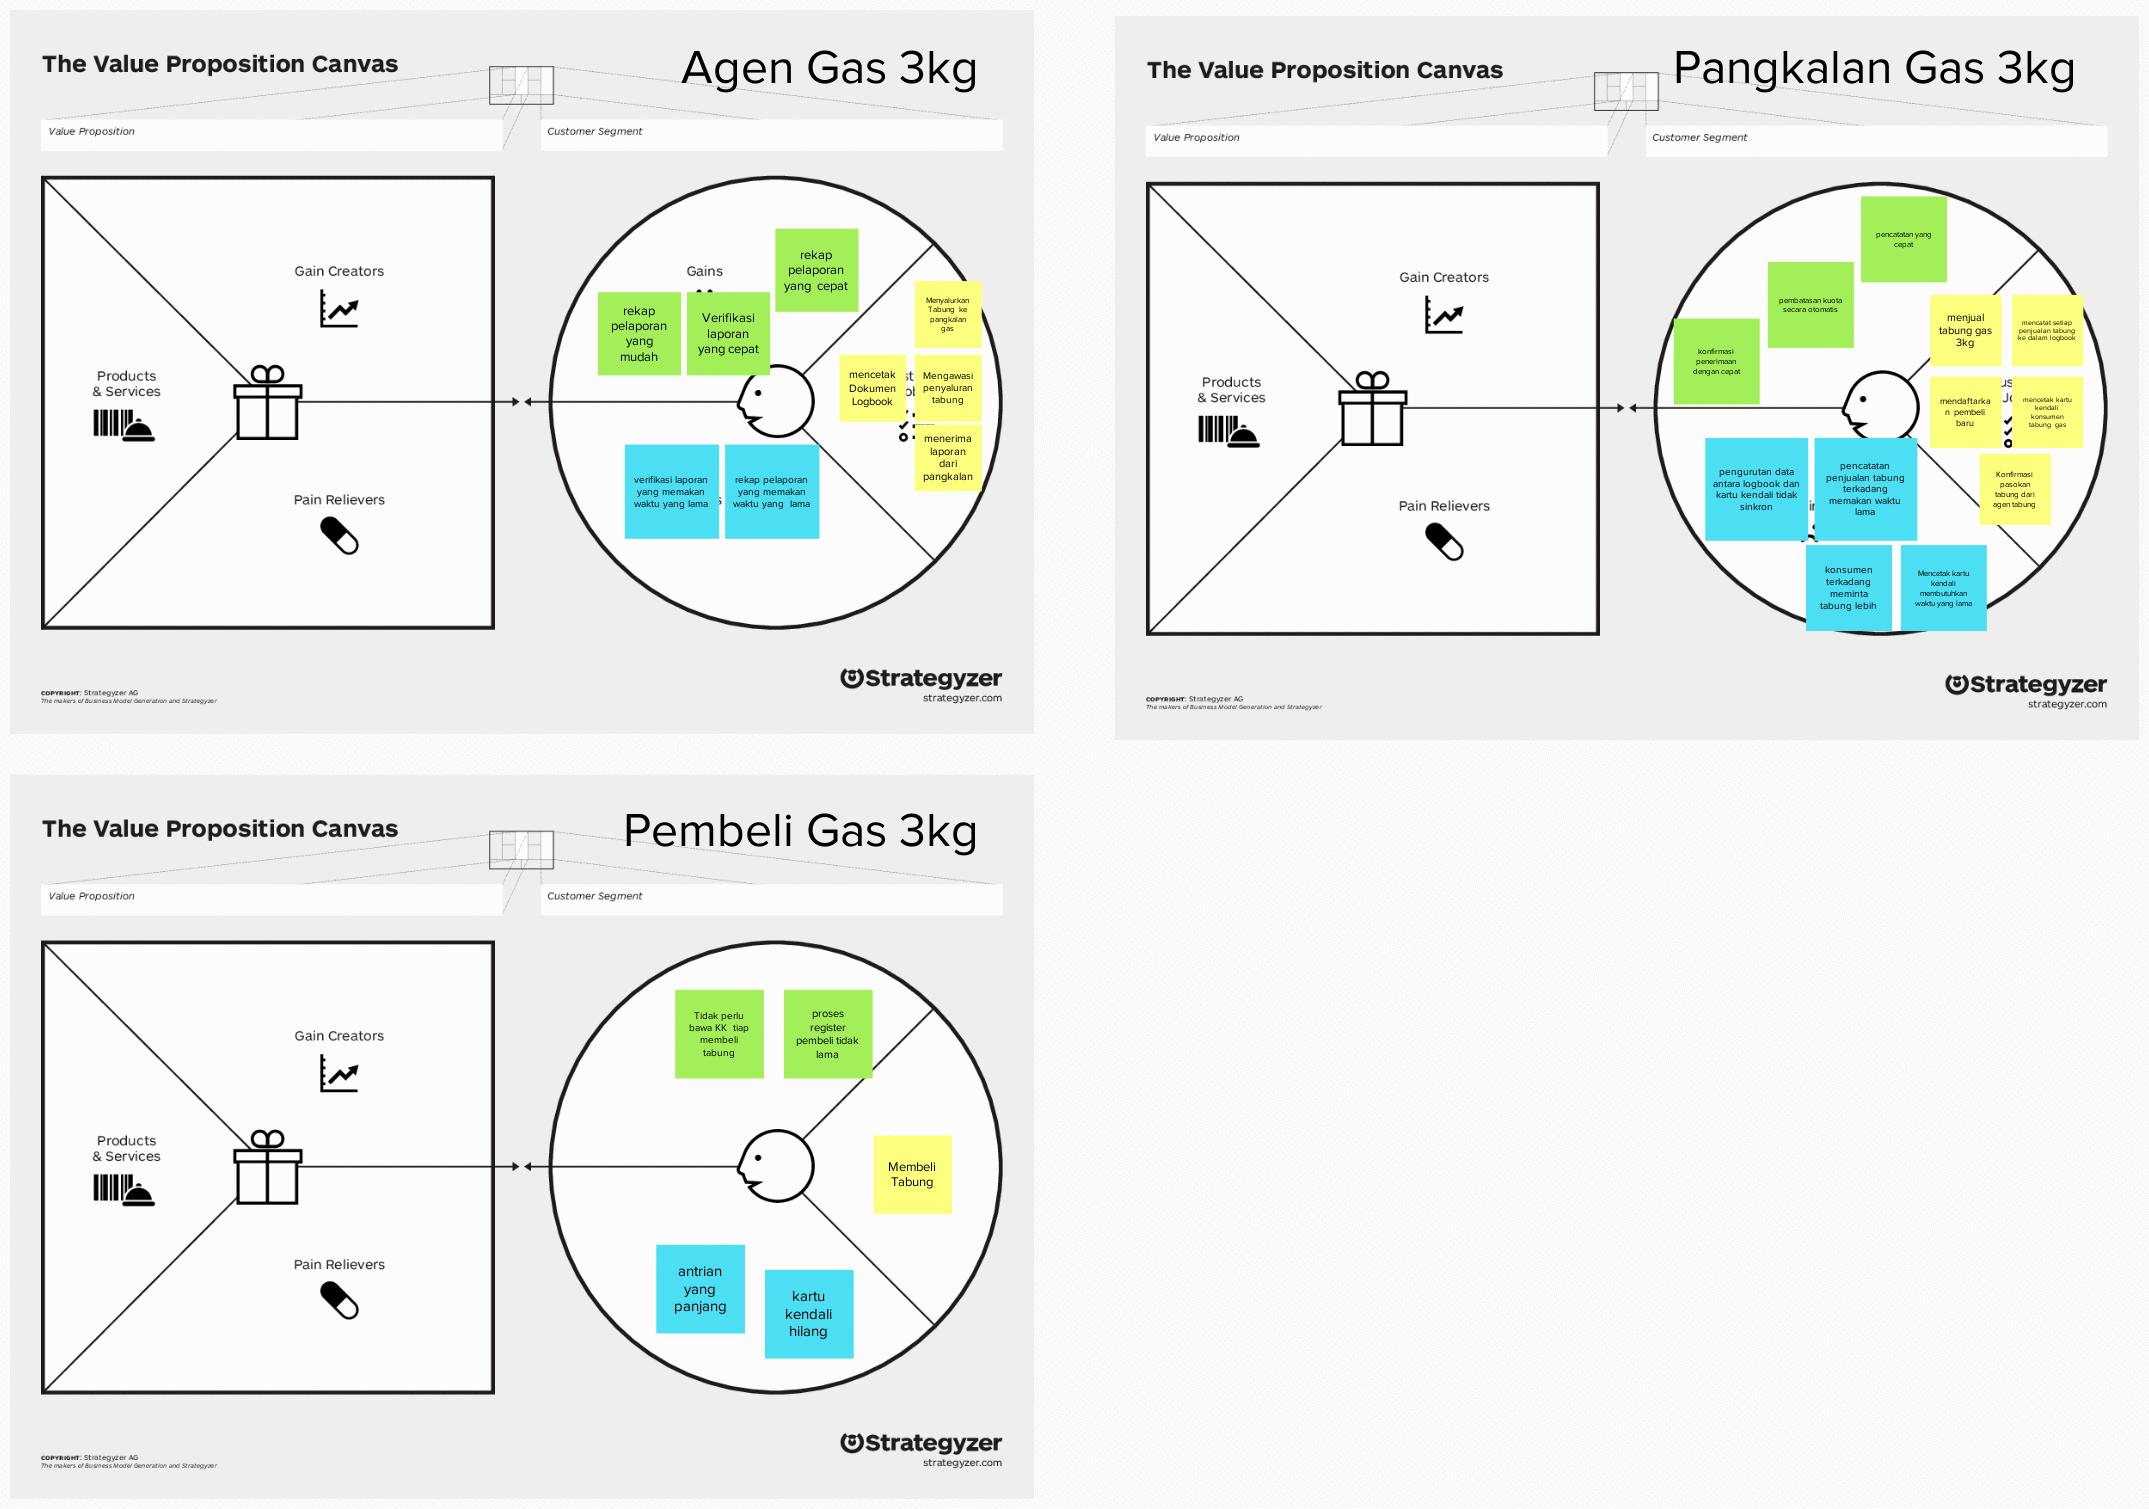
\includegraphics [width = 14cm]{gambar/model/VPC-Gas}
		\caption{Kegiatan Sebelum Menggunakan Aplikasi}
		\label{vpc}
	\end{figure}

	
	\subsection{\textit{Use Case}}
	\textit{Use-Case Diagram} digunakan untuk memetakan fungsionalitas aplikasi pada masing-masing pengguna. Dari hasil pengamatan dapat digambarkan \textit{Use-Case Diagram} sebagai berikut:
	
	\vspace{-0.4cm}
	\begin{figure}[H]
		\center
		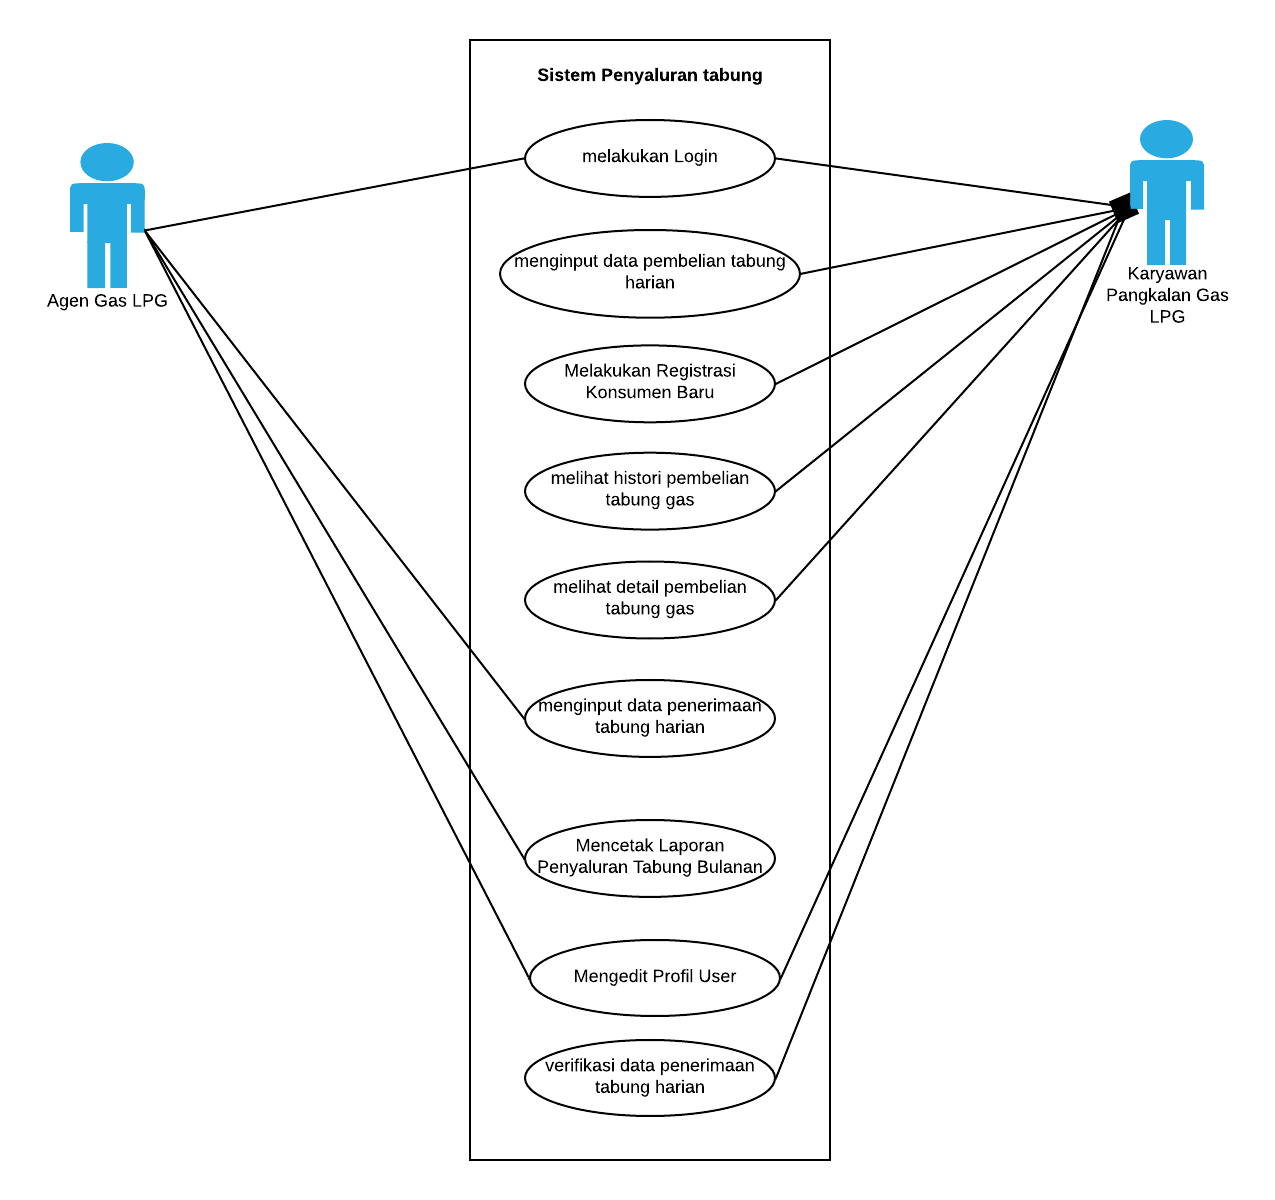
\includegraphics [width = 14cm]{gambar/model/use-case-diagram}
		\caption{Use-Case Diagram}
		\label{usecase}
	\end{figure}
	
	\section{Desain dan Pembuatan Sistem}
	
	\subsection{Desain Sistem}
	\par Desain Sistem adalah proses desain pada aplikasi yang akan dibangun. proses dilakukan berdasarkan proses analisis kebutuhan aplikasi yang telah dilakukan pada proses sebelumnya. proses ini terdiri dari beberapa tahap yaitu seperti perancangan \textit{deployment diagram},
	perancangan arsitektur aplikasi dalam bentuk \textit{component diagram}, perancangan struktur basis data dalam bentuk \textit{class diagram}, dan juga perancangan tampilan antar muka dari aplikasi yang akan dibangun.
	
	\par tahap pertama adalah merancang \textit{deployment diagram}, dimana \textit{deployment diagram} adalah diagram yang menjelaskan bagaimana sistem aplikasi akan bekerja dan digunakan oleh pengguna. aplikasi yang dibangun terdiri dari 2 platform yang berbeda dimana pengguna pangkalan akan menggunakan platform android untuk melakukan pencatatan penjualan tabung, dan lain-lain, sedangkan pengguna agen akan menggunakan platform \textit{web-based} untuk rekapitulasi laporan penyaluran. Berikut rancangan \textit{deployment diagram} yang telah dibuat:
	
		\vspace{-0.4cm}
	\begin{figure}[H]
		\center
		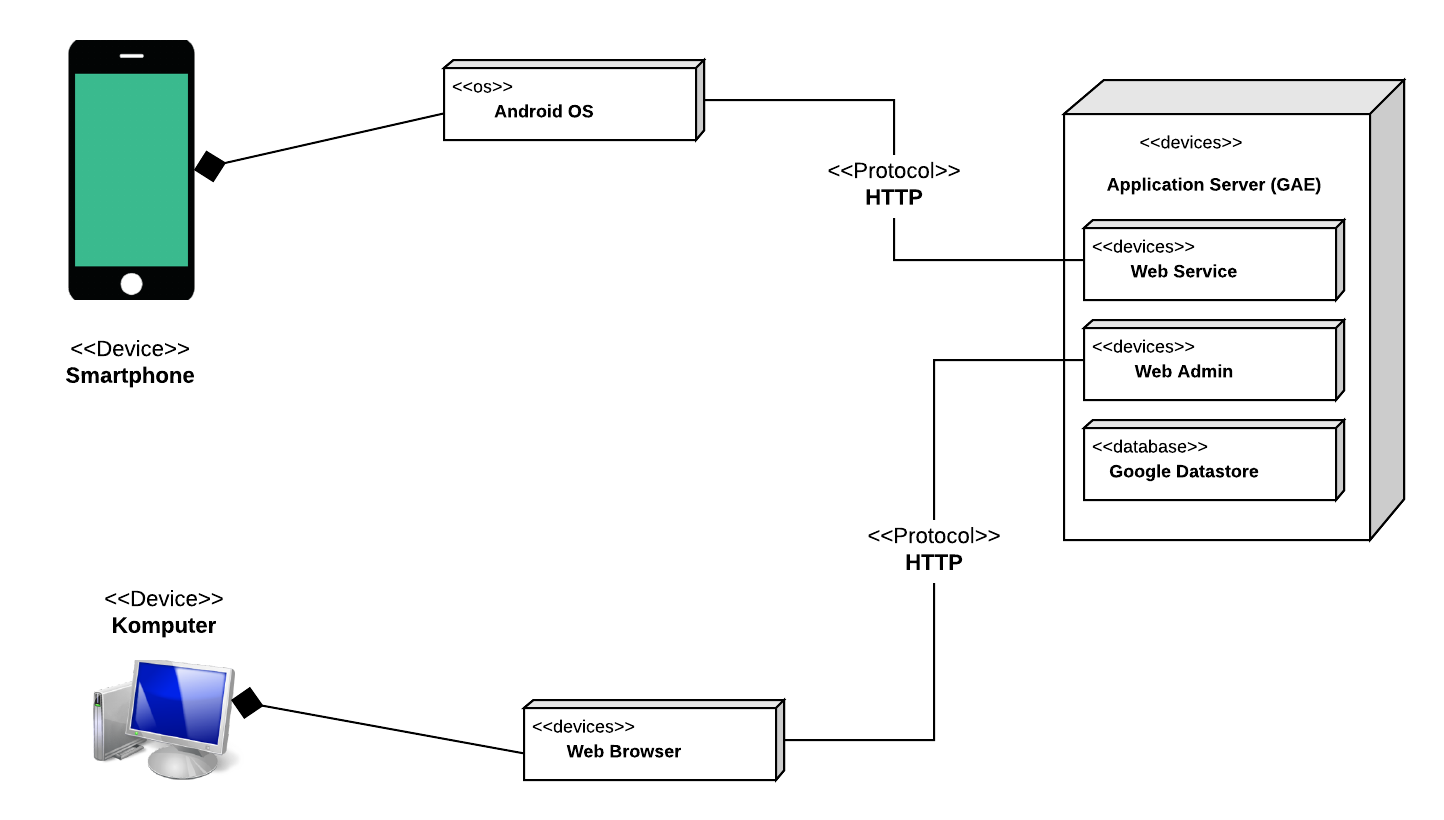
\includegraphics [width = 14cm]{gambar/model/deployment}
		\caption{Diagram Deployment}
		\label{deployment}
	\end{figure}

	\par tahap selanjutnya adalah merancang \textit{component diagram}, dimana \textit{component diagram} adalah diagram yang menjelaskan arsitektur sistem aplikasi yang akan dibangun secara keseluruhan. Berikut rancangan \textit{component diagram} yang telah dibuat:
	
	\vspace{-0.4cm}
	\begin{figure}[H]
		\center
		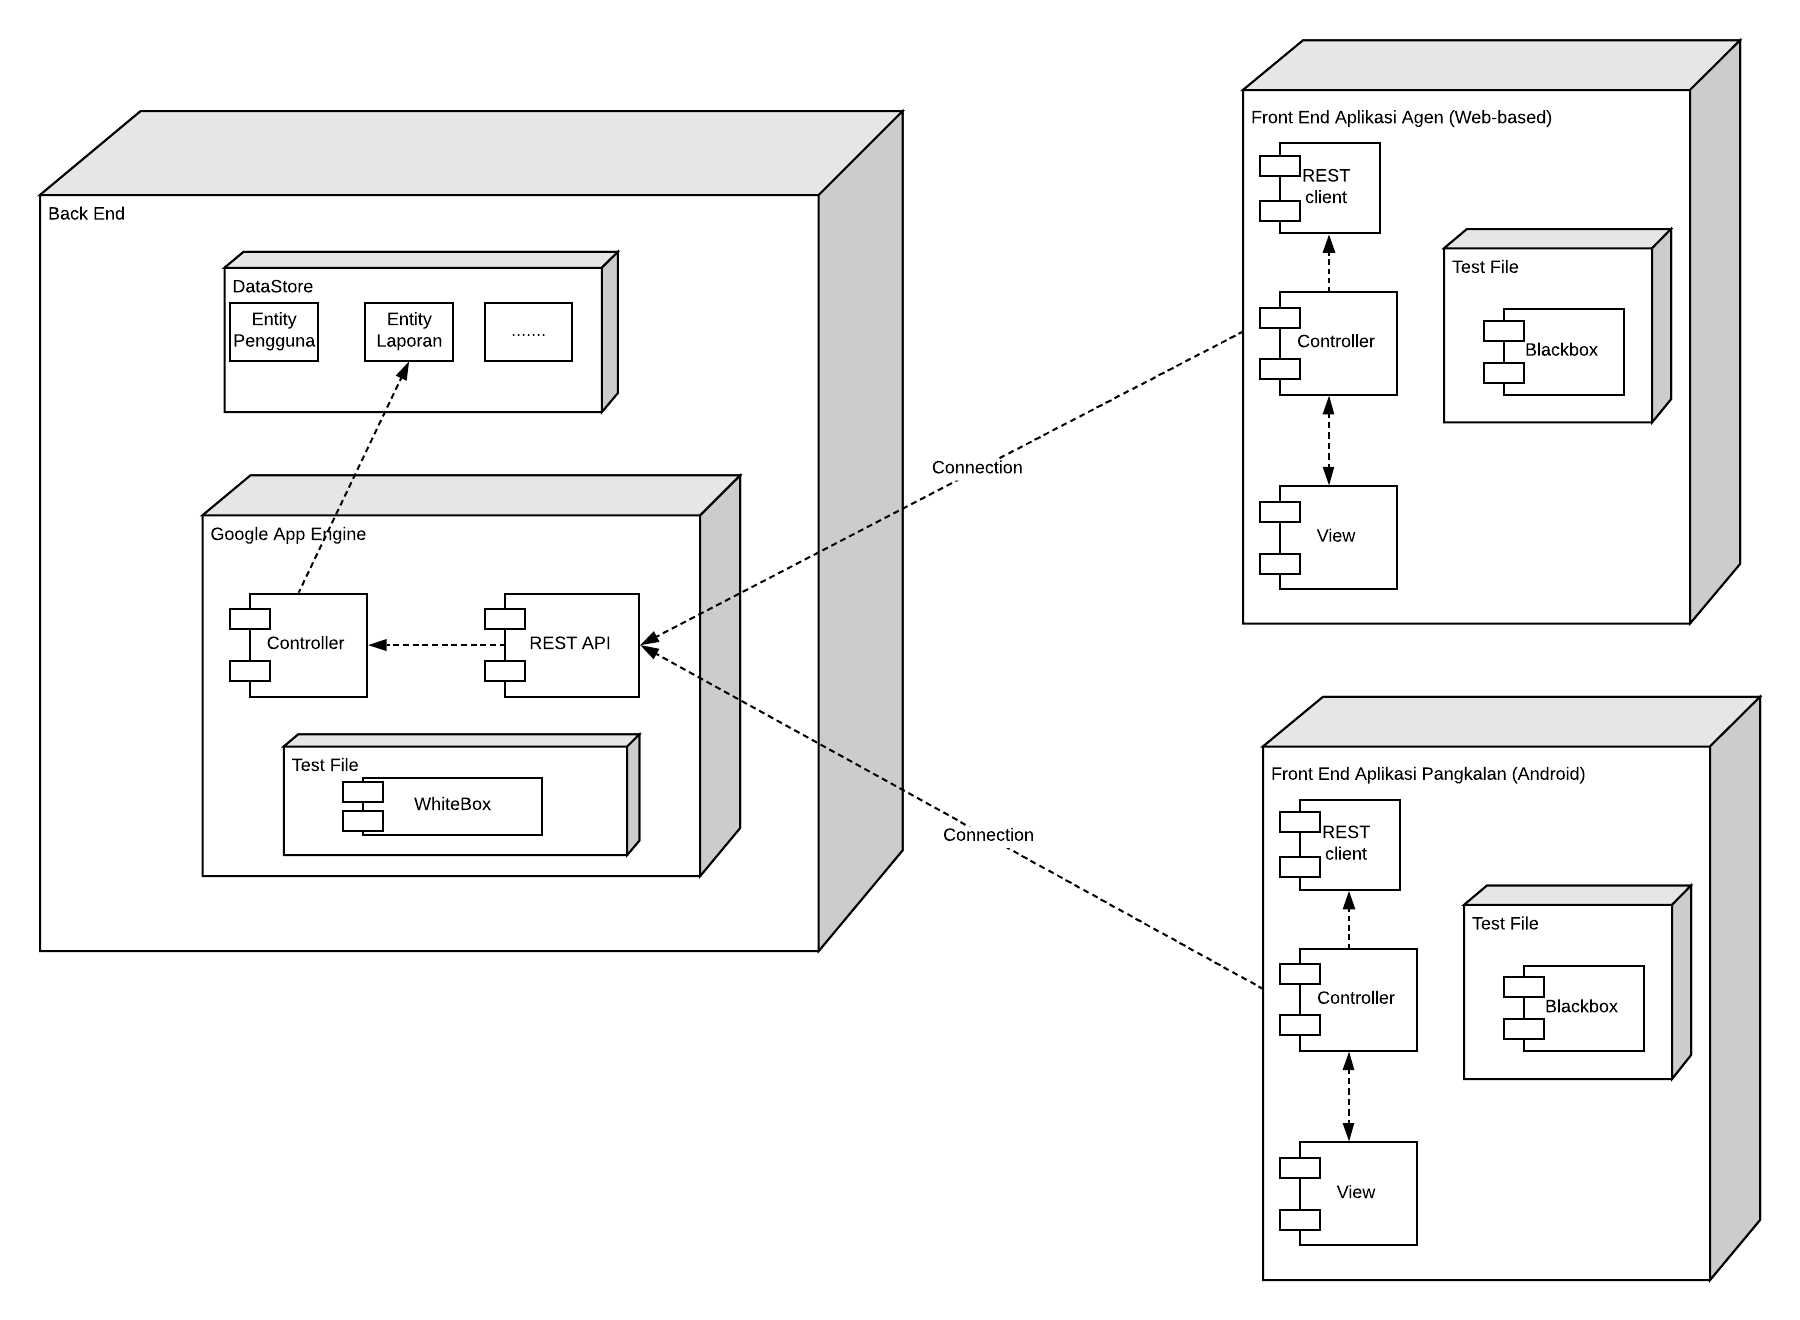
\includegraphics [width = 14cm]{gambar/model/component}
		\caption{Diagram Component}
		\label{component}
	\end{figure}

	\pagebreak
	\par Dilanjutkan dengan tahap perancangan model basis data menggunakan \textit{class diagram}. diagram ini dibuat berdasarkan fungsionalitas dari sistem yang akan dibangun. Berikut rancangan \textit{class diagram} yang telah dibuat:
	
		\vspace{-0.4cm}
	\begin{figure}[H]
		\center
		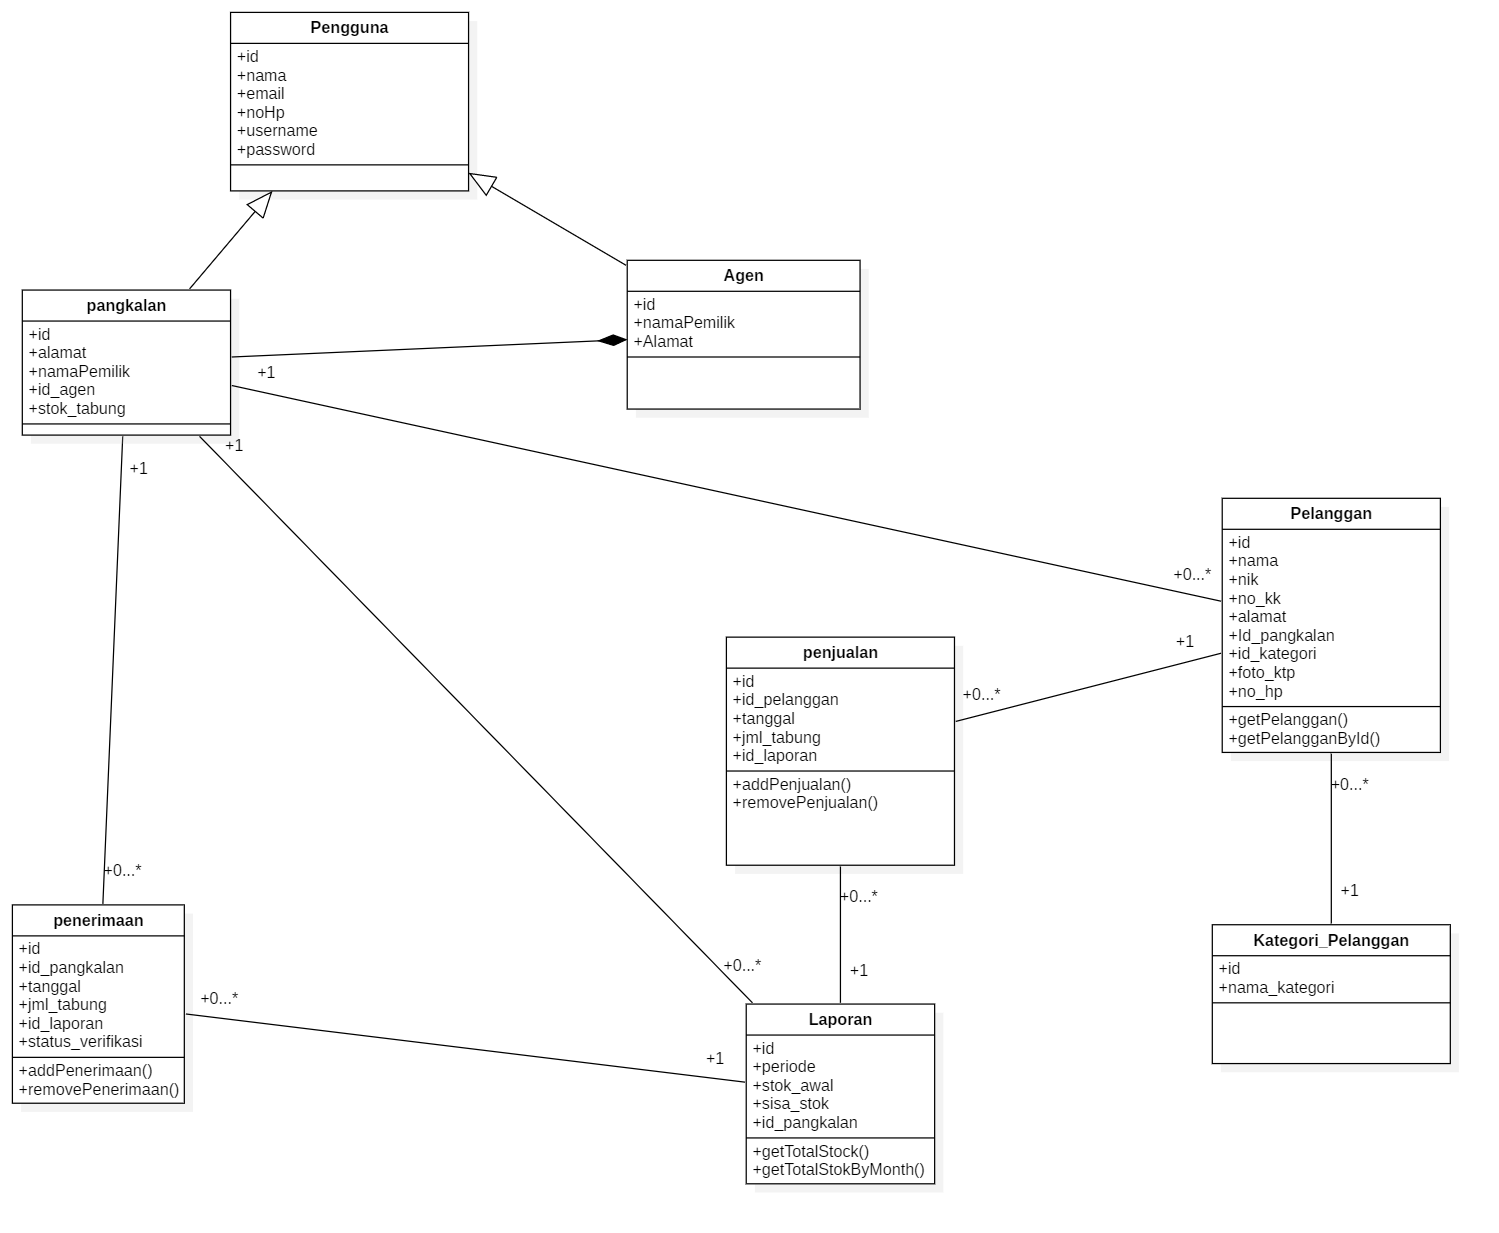
\includegraphics [width = 14cm]{gambar/model/class-diagram}
		\caption{Diagram Kelas Model Basis Data }
		\label{class}
	\end{figure}

	\par Selanjutnya adalah perancangan layanan web, perancangan layanan web disini memiliki peran yang sangat penting dan vital, dimana layanan web harus dapat menangani setiap proses transaksi data yang dilakukan oleh sistem. layanan web ini menggunakan RESTful API untuk dapat berinteraksi dengan \textit{platform} android dan aplikasi lain melalui HTTP URL.
	
	\par Untuk perancangan antar muka dari aplikasi ini menggunakan ionic framework karena menyediakan komponen-komponen antar muka pengguna seperti \textit{tabs, card, dan button} yang cocok untuk digunakan pada platform \textit{mobile}.
	
	\par Tampilan Aplikasi berbasis android untuk pangkalan gas LPG 3Kg ini terdiri 3 halaman utama yaitu halaman register pelanggan baru, halaman pembelian tabung, dan halaman penerimaan tabung. Pertama-tama untuk masuk ke dalam aplikasi, pangkalan harus melakukan \textit{login} menggunakan no HP yang telah terdaftar seperti pada gambar \ref{tampilanLoginPangkalan}. setelah itu akan muncul sms no HP tersebut berisi sebuah kode OTP(\textit{One Time Password}) yang digunakan untuk verifikasi no HP valid atau tidak. setelah proses \textit{login} berhasil maka dilanjut ke halaman beranda yang berisi menu utama aplikasi seperti pada Gambar \ref{tampilanBerandaPangkalan}.
	\par Pada halaman registrasi pelanggan baru terdapat \textit{form} mengenai data pelanggan setelah itu dilanjutkan pengambilan foto ktp dan foto diri pelanggan seperti pada Gambar \ref{tampilanRegisterPangkalan}. Pada saat pembelian tabung, pangkalan harus mencari pelanggan terlebih dahulu menggunakan NIK (Nomor Induk Kependudukan) seperti pada Gambar \ref{tampilanPembelianPangkalan} setelah itu maka akan muncul halaman detail pelanggan berisi detail data pelanggan tersebut. pada halaman ini terdapat 2 tombol aksi yaitu riwayat pembelian dan beli tabung seperti pada Gambar \ref{tampilanPembelianPangkalan}. setelah pangkalan memilih beli tabung selanjutnya pangkalan harus memilih jumlah tabung yang dibeli dan dilanjutkan pengambilan foto pembeli sebagai bukti pembelian seperti pada Gambar \ref{tampilanPembelianPangkalan}. Pada saat penerimaan pasokan tabung, pangkalan harus melakukan verifikasi penerimaan tabung pada menu penerimaan tabung seperti pada Gambar \ref{tampilanPenerimaanPangkalan}.
	
	\vspace{-0.2cm}
	\begin{figure}[H]
		\center
		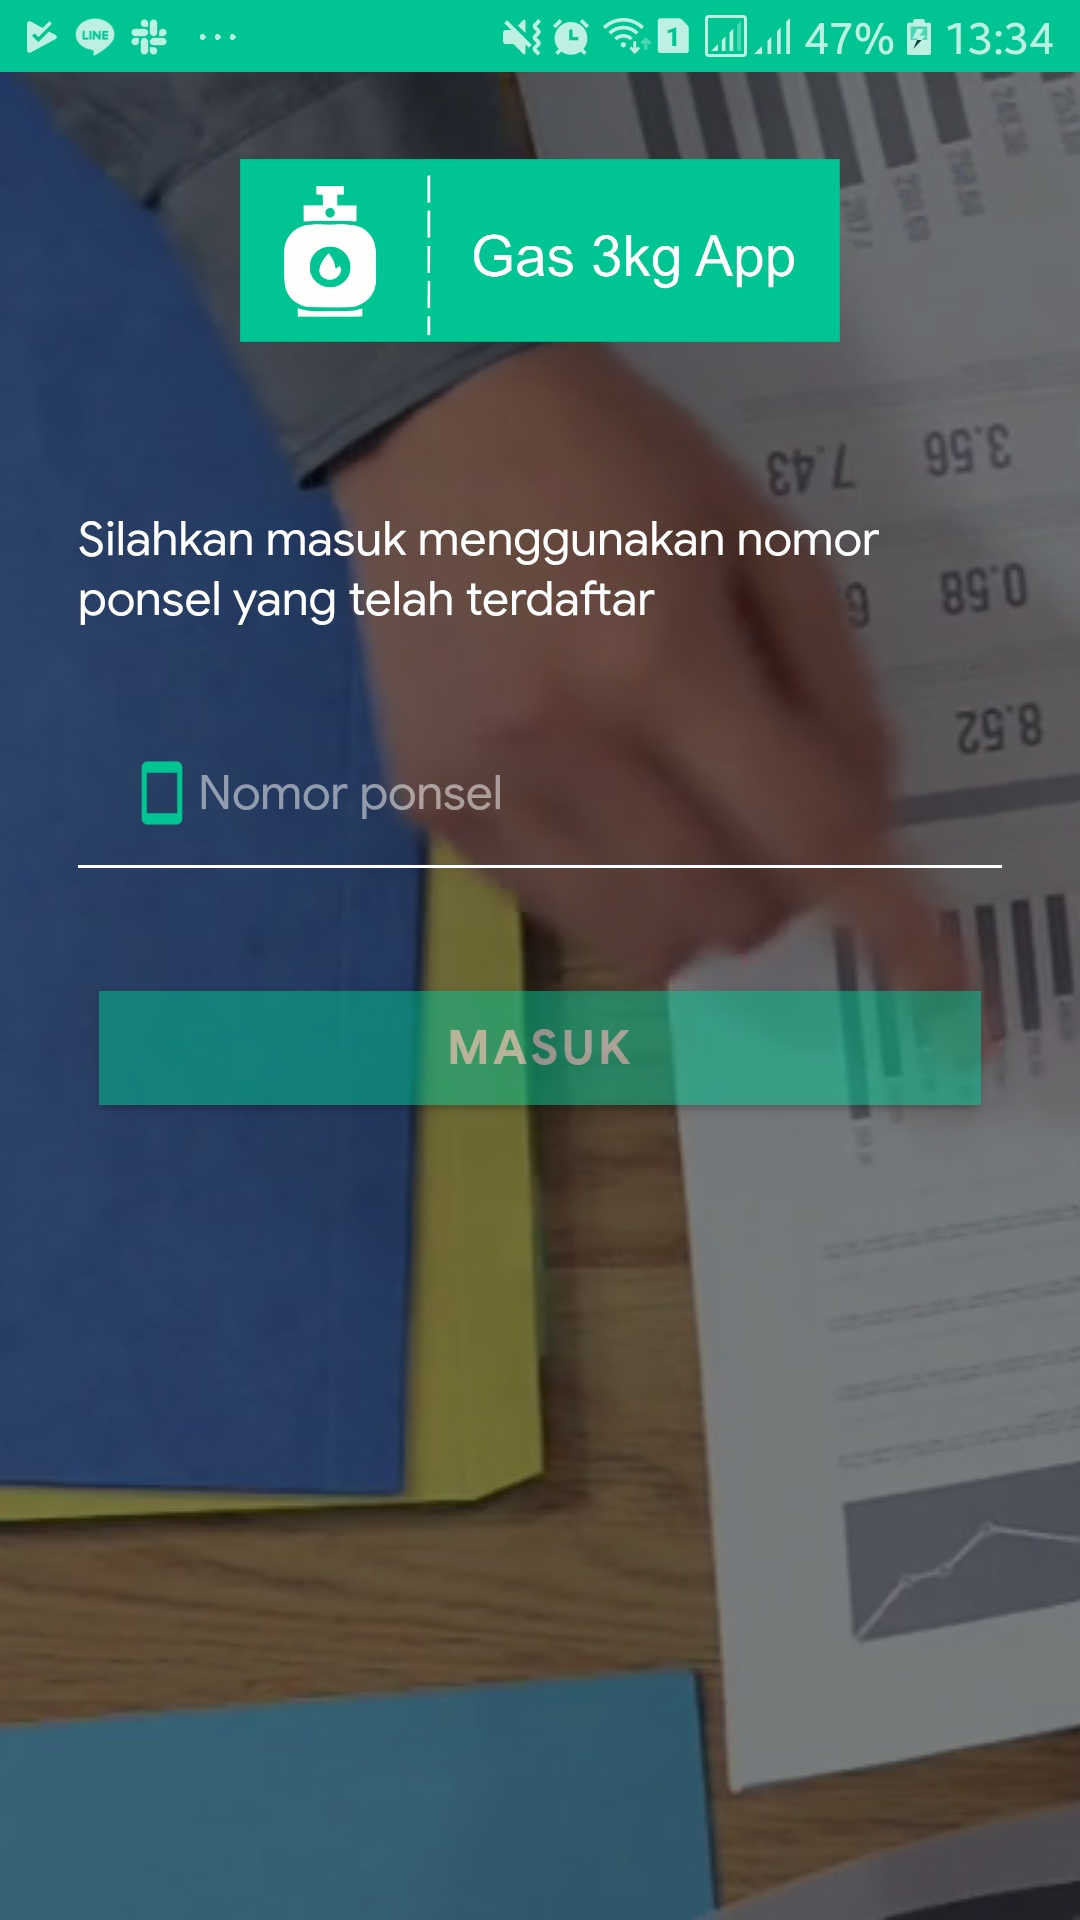
\includegraphics [width = 7cm]{gambar/android/login}
		\vspace{1cm}
		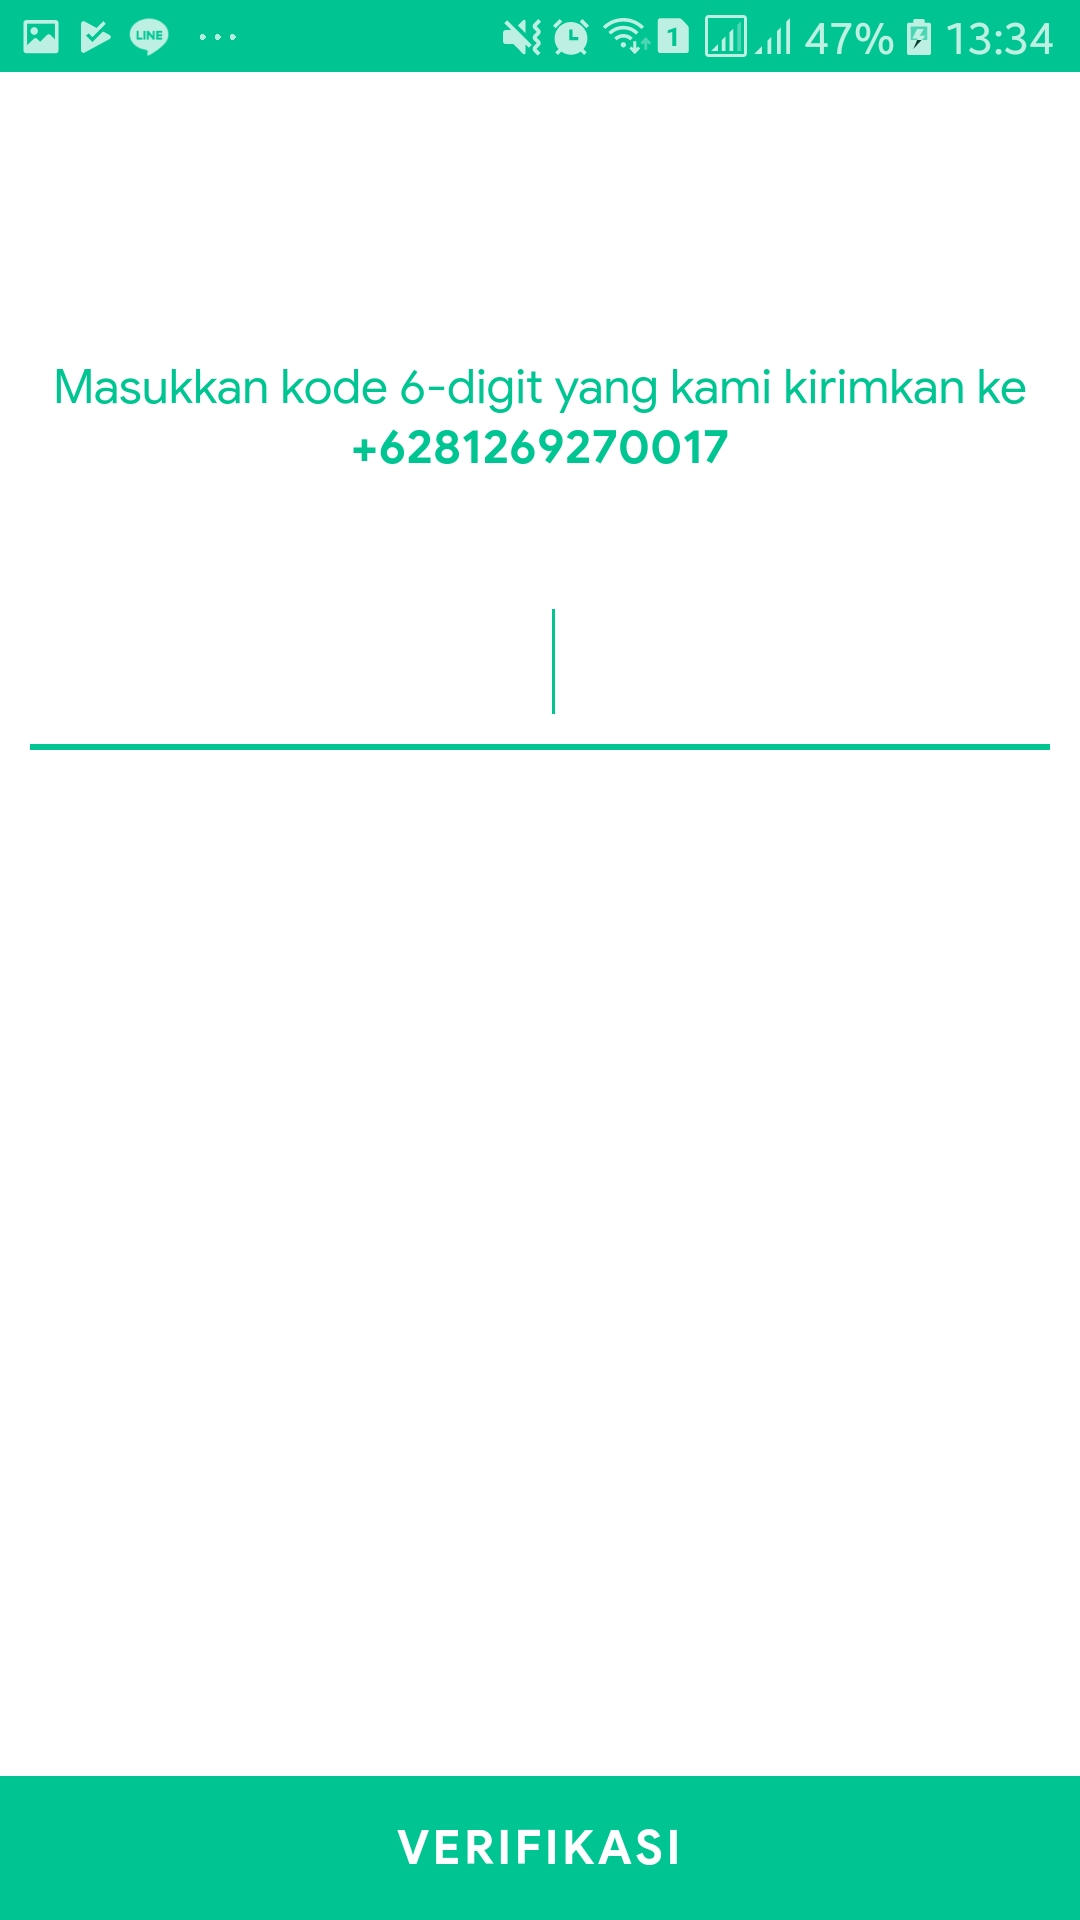
\includegraphics [width = 7cm]{gambar/android/verify}
		\caption{Tampilan Login aplikasi}
		\label{tampilanLoginPangkalan}
	\end{figure}
	
	\begin{figure}[H]
		\center
		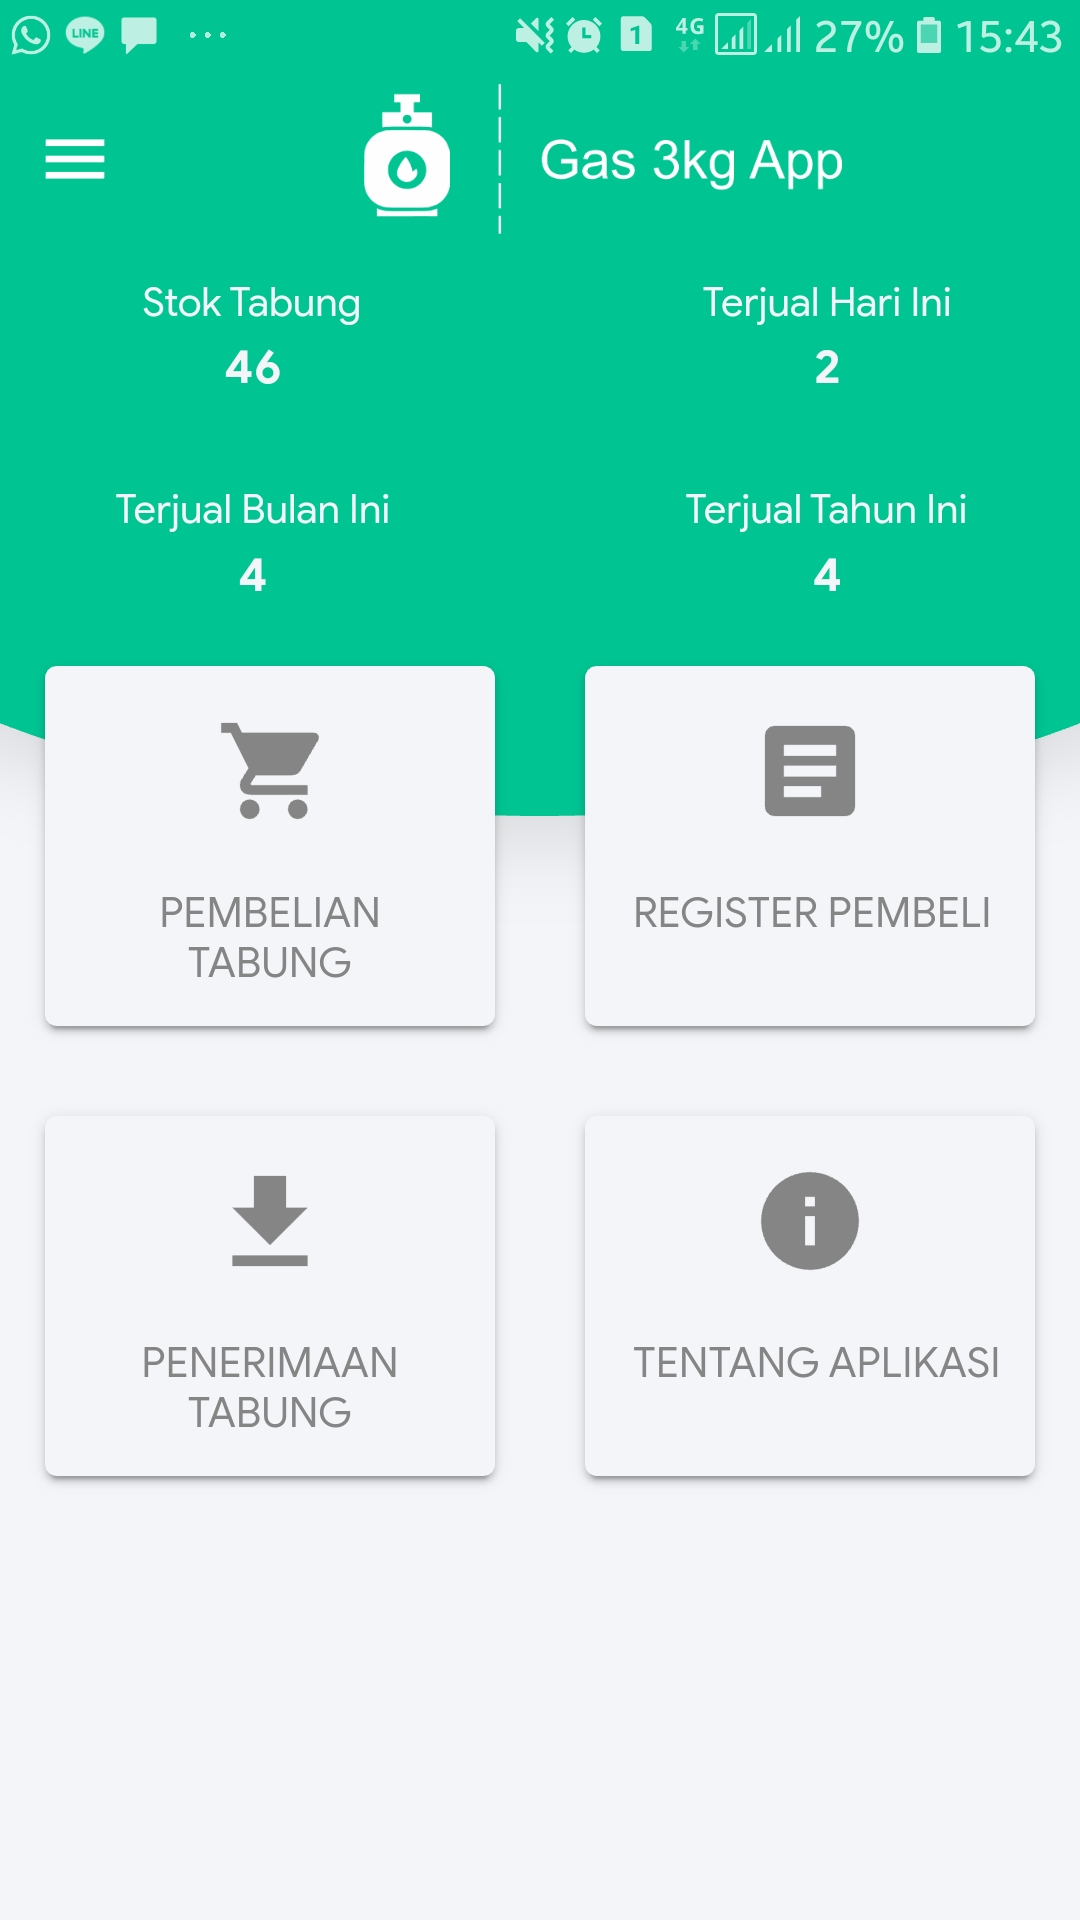
\includegraphics [width = 7cm]{gambar/android/beranda}
		\caption{Tampilan Halaman Beranda}
		\label{tampilanBerandaPangkalan}
	\end{figure}

	\begin{figure}[H]
		\center
		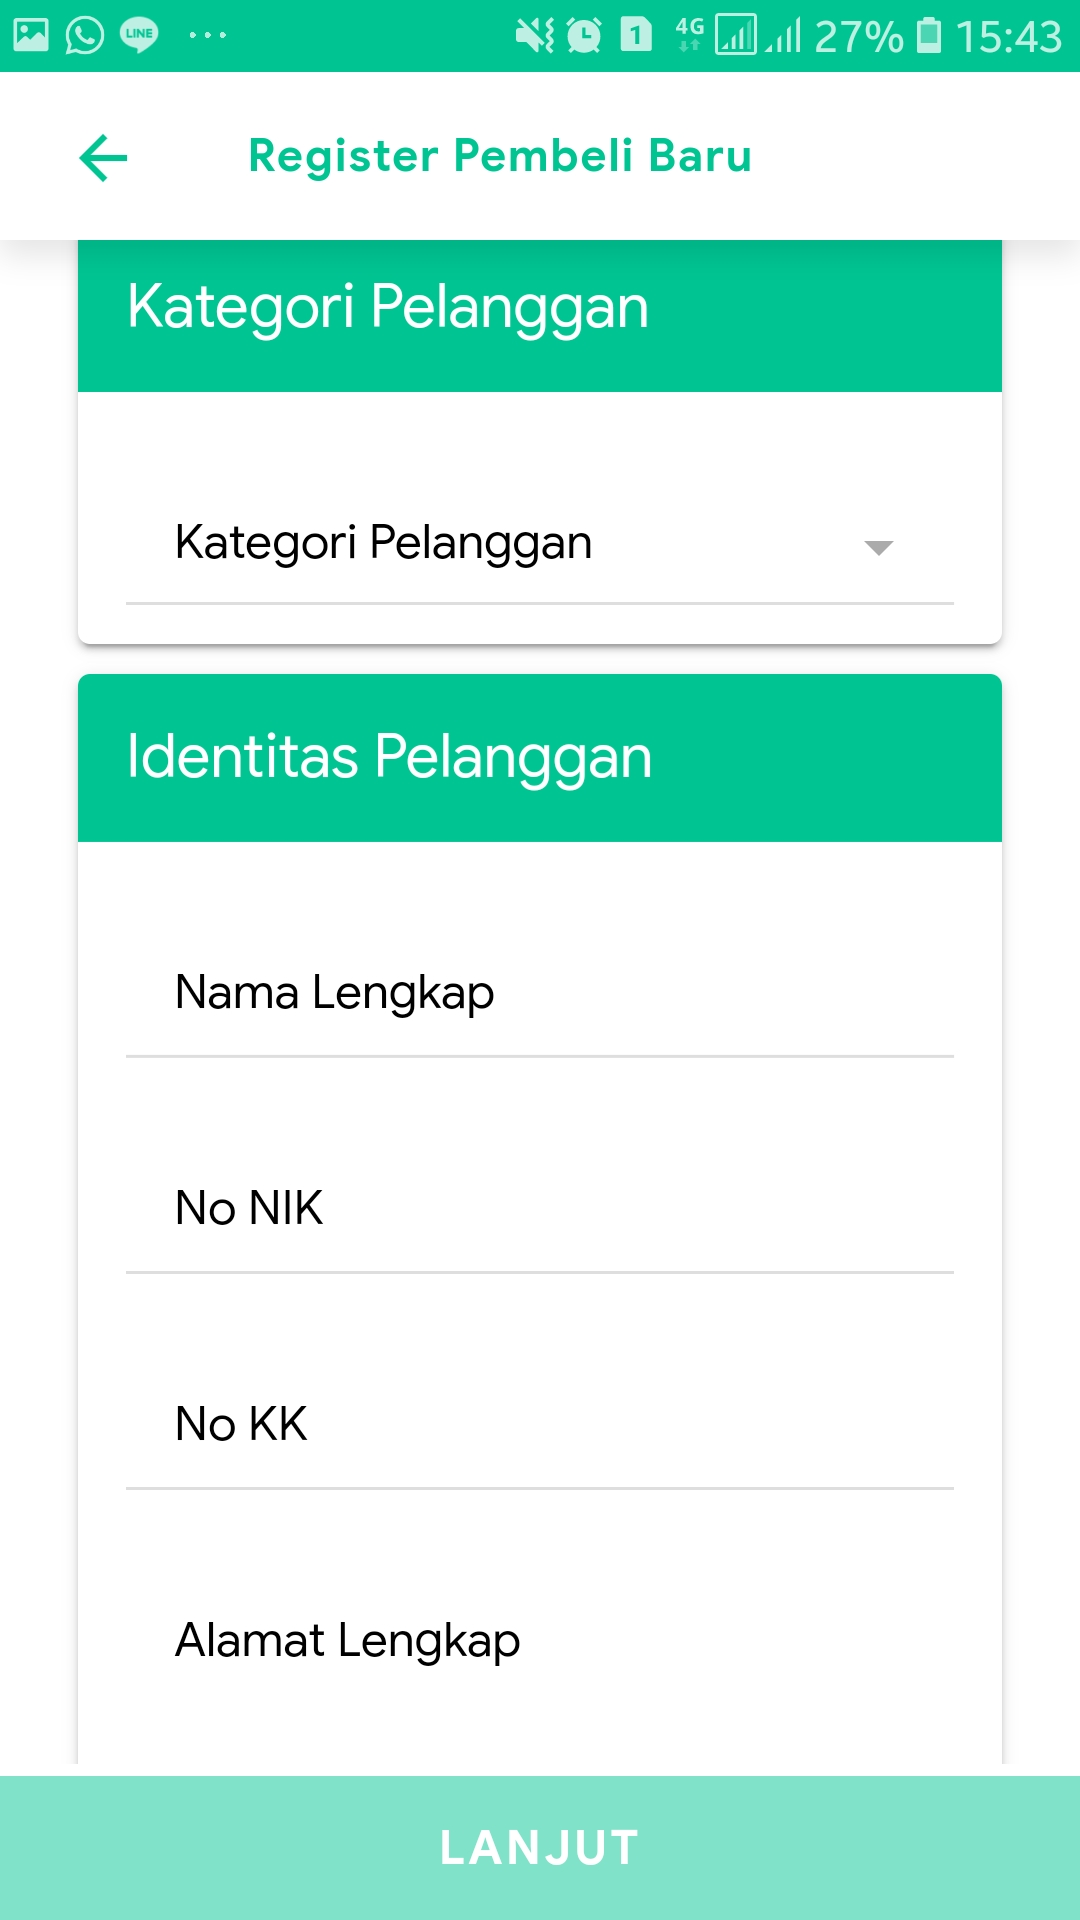
\includegraphics [width = 6cm]{gambar/android/register}
		\caption{Tampilan Halaman Register Pelanggan}
		\label{tampilanRegisterPangkalan}
	\end{figure}

	\begin{figure}[H]
		\center
		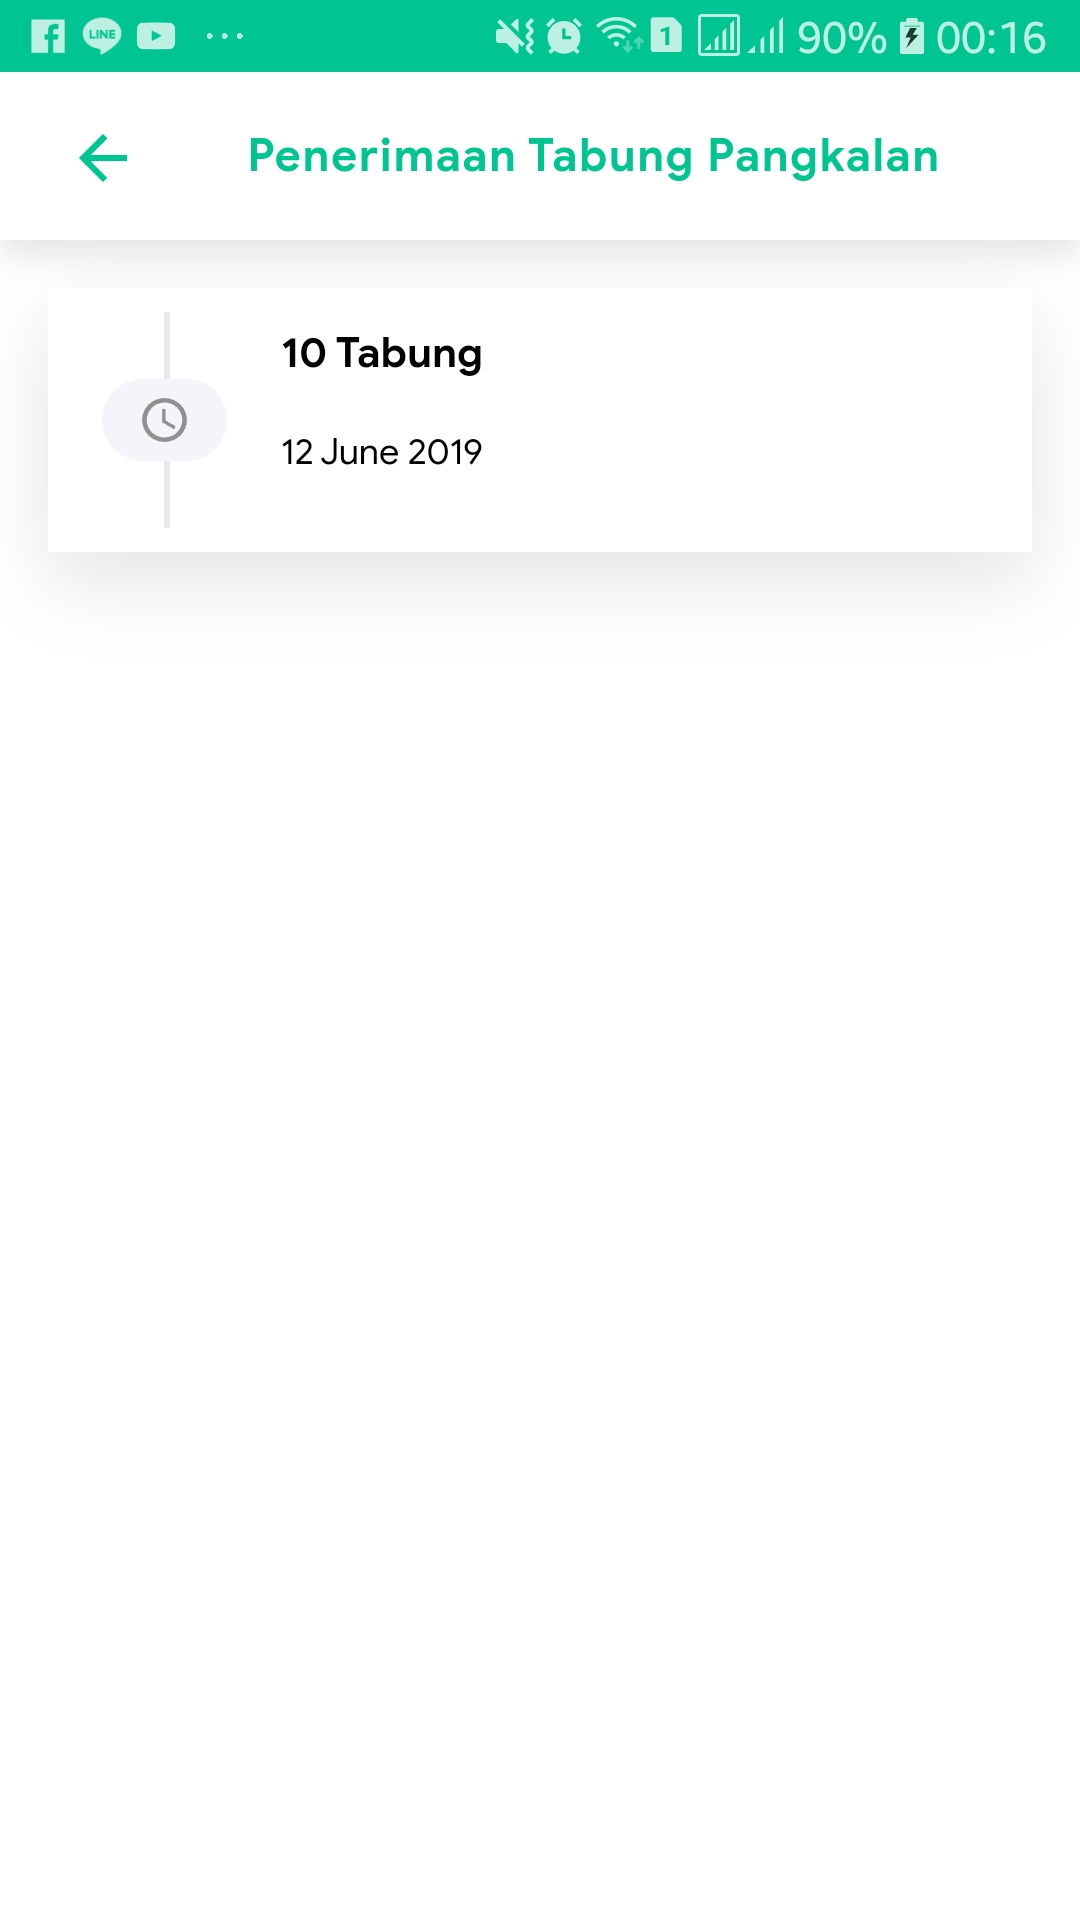
\includegraphics [width = 6cm]{gambar/android/penerimaan}
		\caption{Tampilan Halaman Penerimaan Pasokan Tabung}
		\label{tampilanPenerimaanPangkalan}
	\end{figure}

	\begin{figure}[H]
		\center
		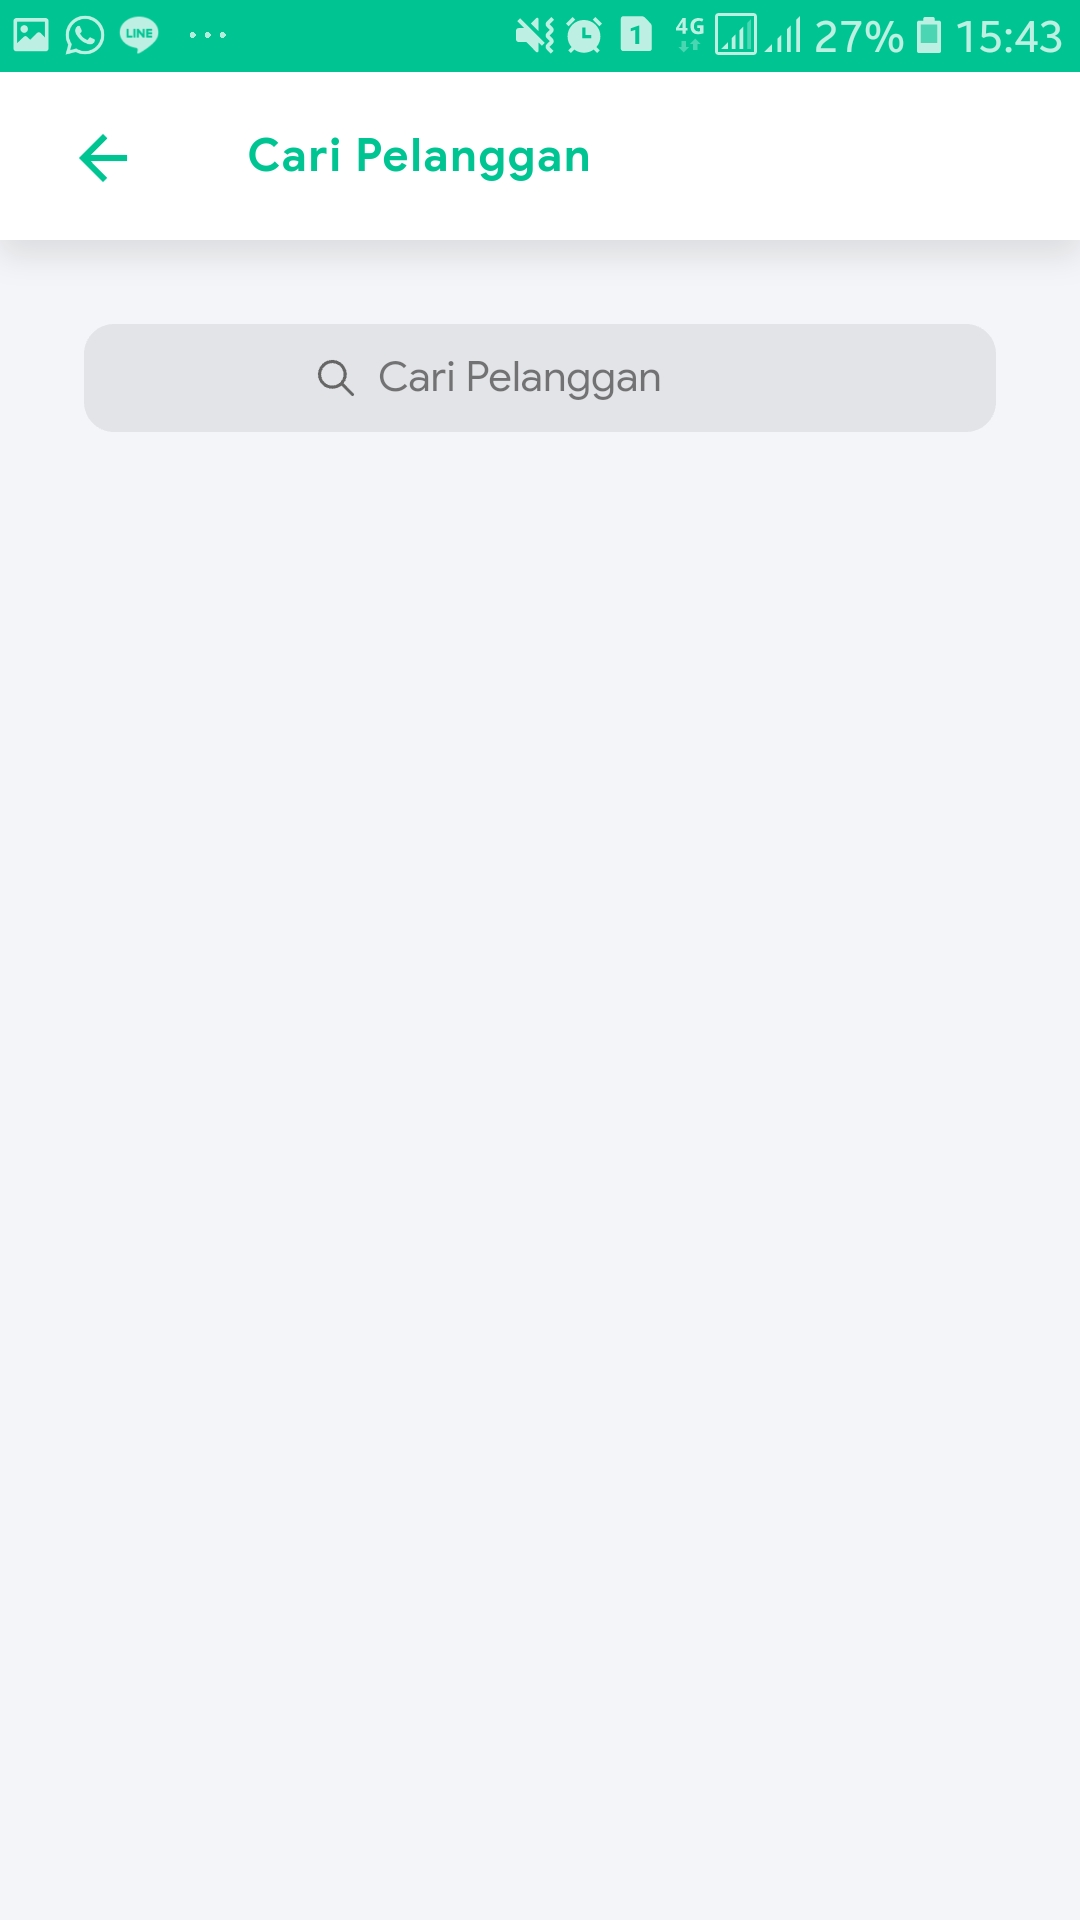
\includegraphics [width = 6cm]{gambar/android/cari-pelanggan}
		\vspace{1cm}
		\hspace{1cm}
		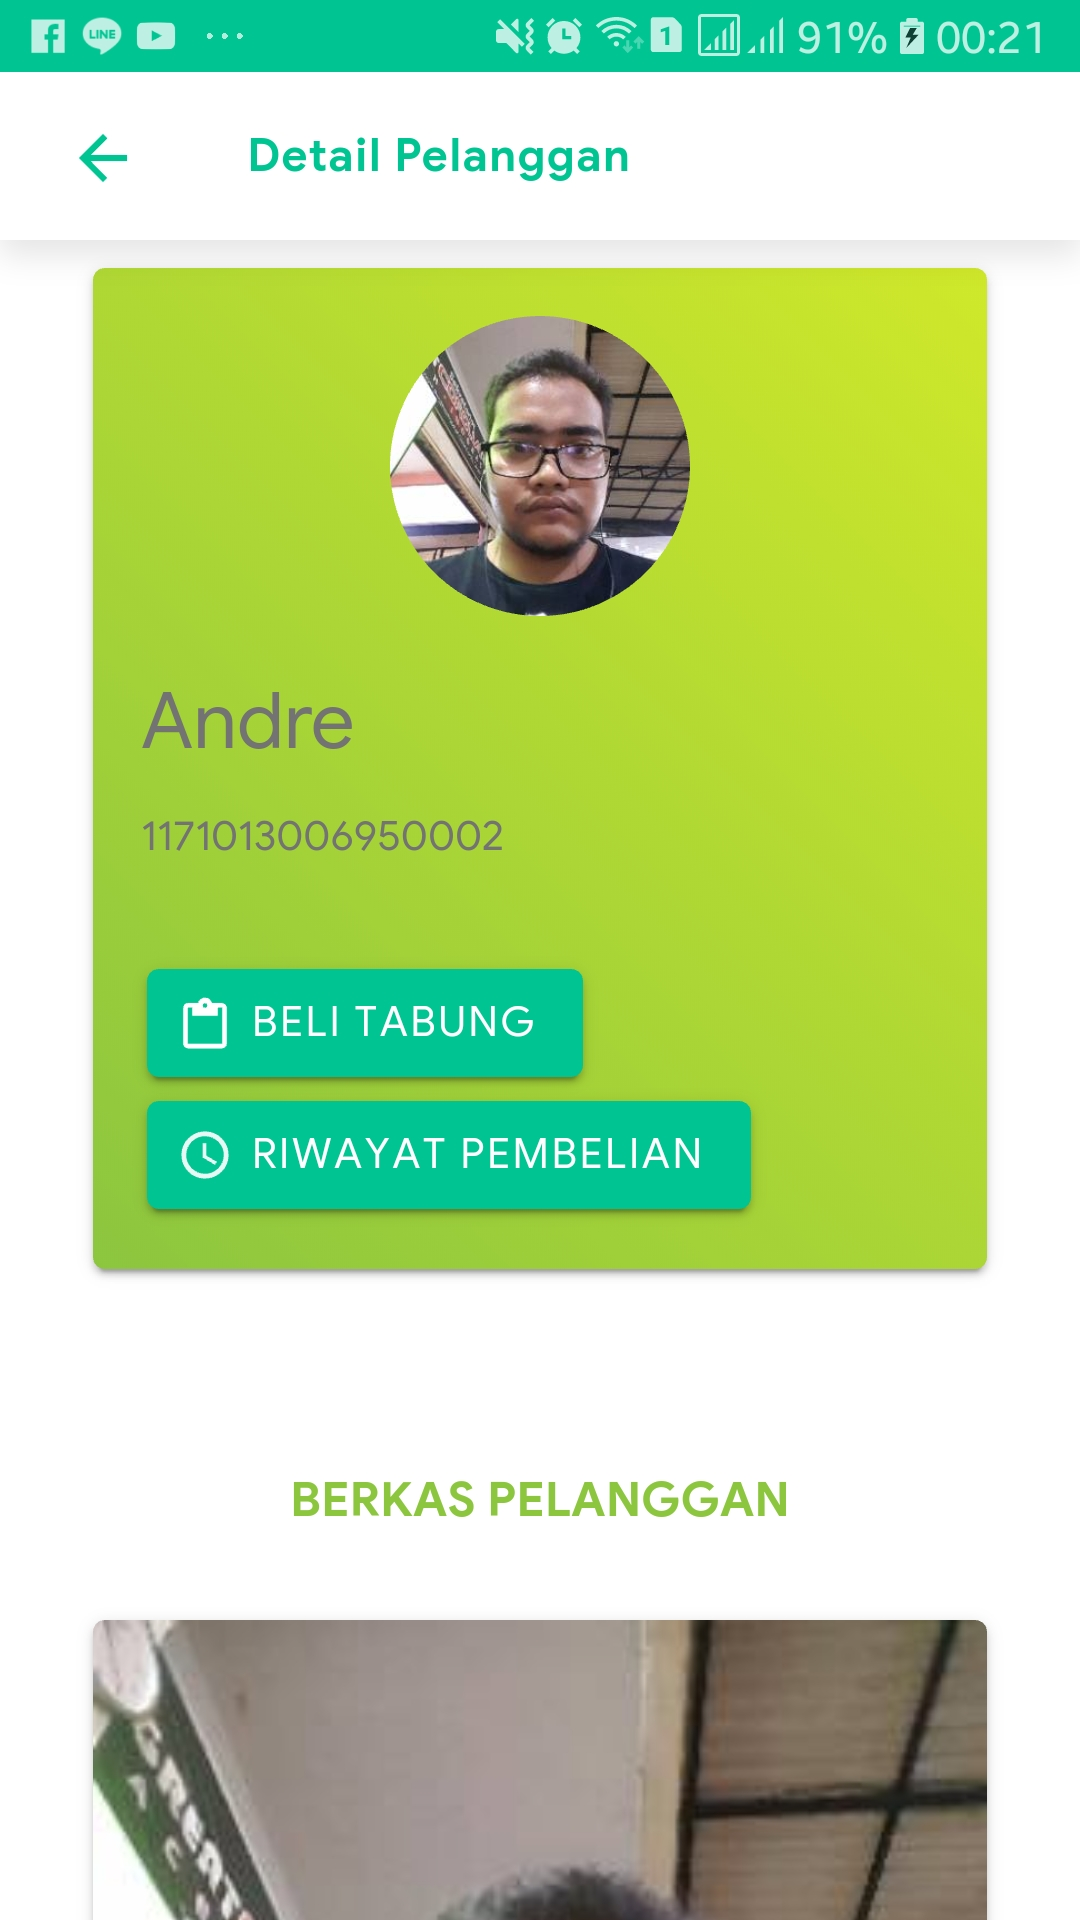
\includegraphics [width = 6cm]{gambar/android/detail-pelanggan}
		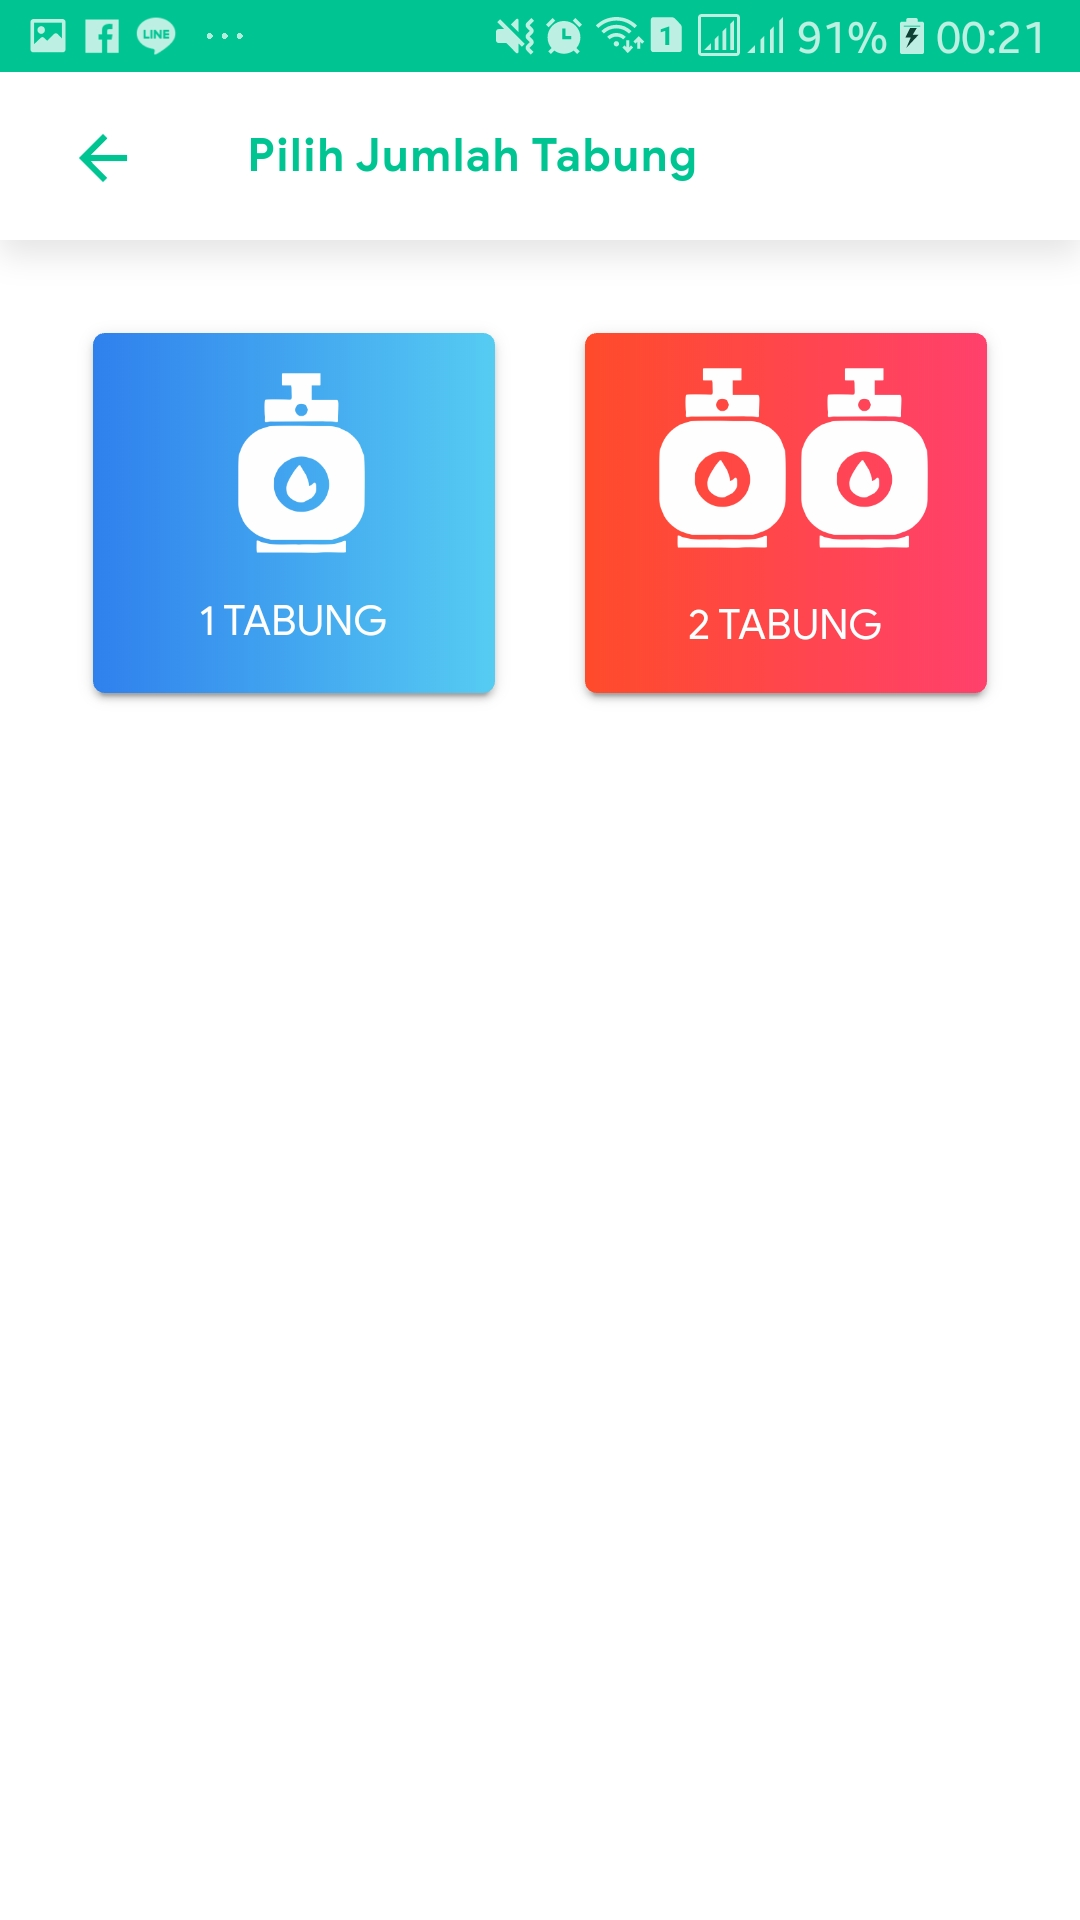
\includegraphics [width = 6cm]{gambar/android/pilih-tabung}
		\hspace{1cm}
		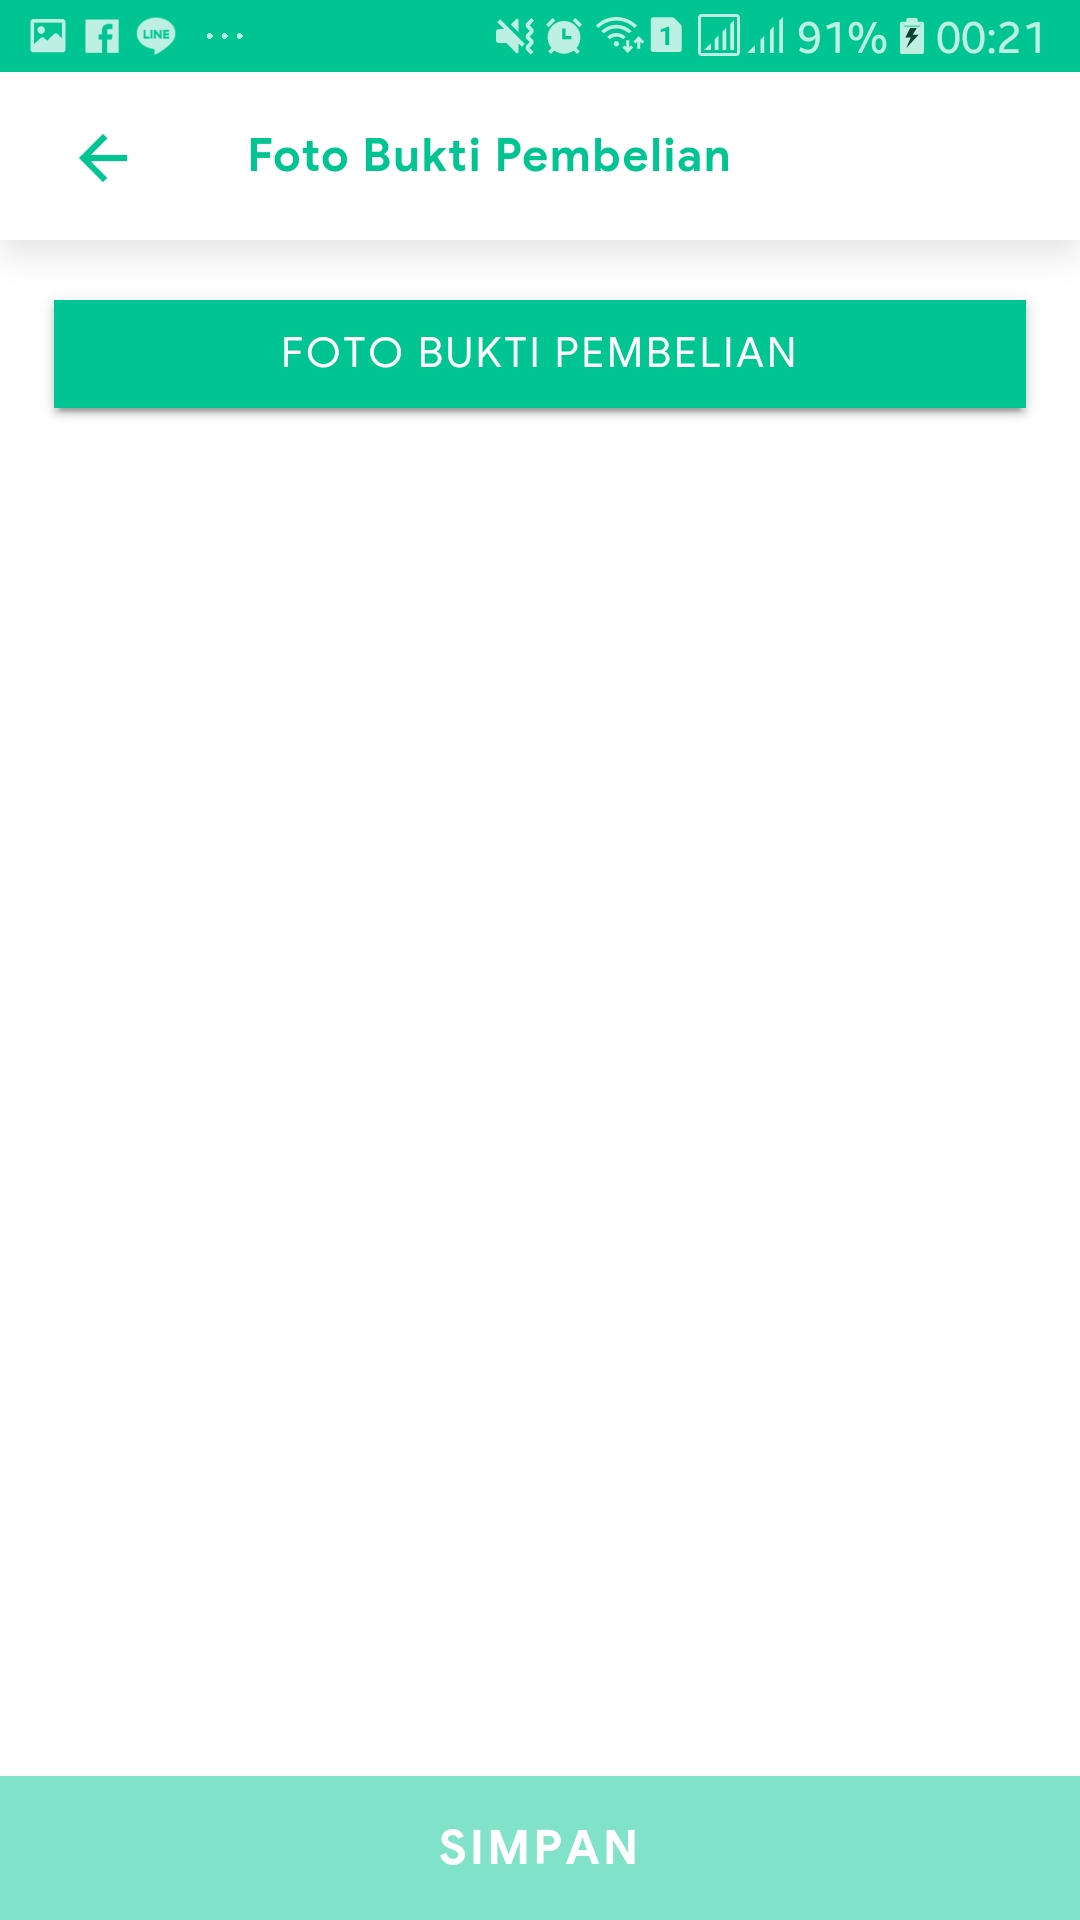
\includegraphics [width = 6cm]{gambar/android/bukti-pembelian}
		\caption{Tampilan Halaman Pembelian Tabung}
		\label{tampilanPembelianPangkalan}
	\end{figure}

	\par Tampilan Aplikasi berbasis web untuk agen gas LPG 3Kg ini terdiri dari 5 halaman utama yaitu halaman beranda, halaman pangkalan, halaman rencana pasokan tabung, halaman pembeli, dan halaman untuk melakukan ekspor laporan penyaluran.
	\par Sebelumnya masuk ke dalam aplikasi ini, agen harus melakukan login menggunakan email khususnya email google seperti pada Gambar \ref{tampilanLoginAgen}. Setelah berhasil melakukan login maka akan ditujukan ke halaman beranda, pada halaman ini terdapat status jumlah pangkalan, jumlah penjualan rata-rata bulan ini dan tahun ini seperti pada \ref{tampilanBerandaAgen}.
	\par Halaman pangkalan berfungsi untuk menampilkan daftar pangkalan pada agen tersebut, disini agen dapat melakukan penambahan dengan menekan tombol "tambah pangkalan"dan perubahan pada data pangkalan dengan menekan tombol "profil" seperti pada Gambar \ref{tampilanDaftarPangkalanAgen}. Pada halaman ini juga memiliki aksi untuk membuat rencana pasokan tabung untuk pangkalan dengan menekan tombol "rencana pasokan" yang akan ditujukan ke halaman daftar rencana pasokan tabung untuk pangkalan tersebut seperti pada Gambar \ref{tampilanPenerimaanAgen}. Halaman rencana pasokan ini berfungsi untuk menginput data rencana pasokan untuk bulan depan. Data-data ini nantinya harus di verifikasi oleh pangkalan via aplikasi berbasis android sehingga datanya akan tersinkronisasi.
	\par Halaman laporan berfungsi untuk melakukan ekspor laporan penyaluran ke dalam bentuk PDF seperti pada Gambar \ref{tampilanLaporanAgen}.
	
	\begin{figure}[H]
		\center
		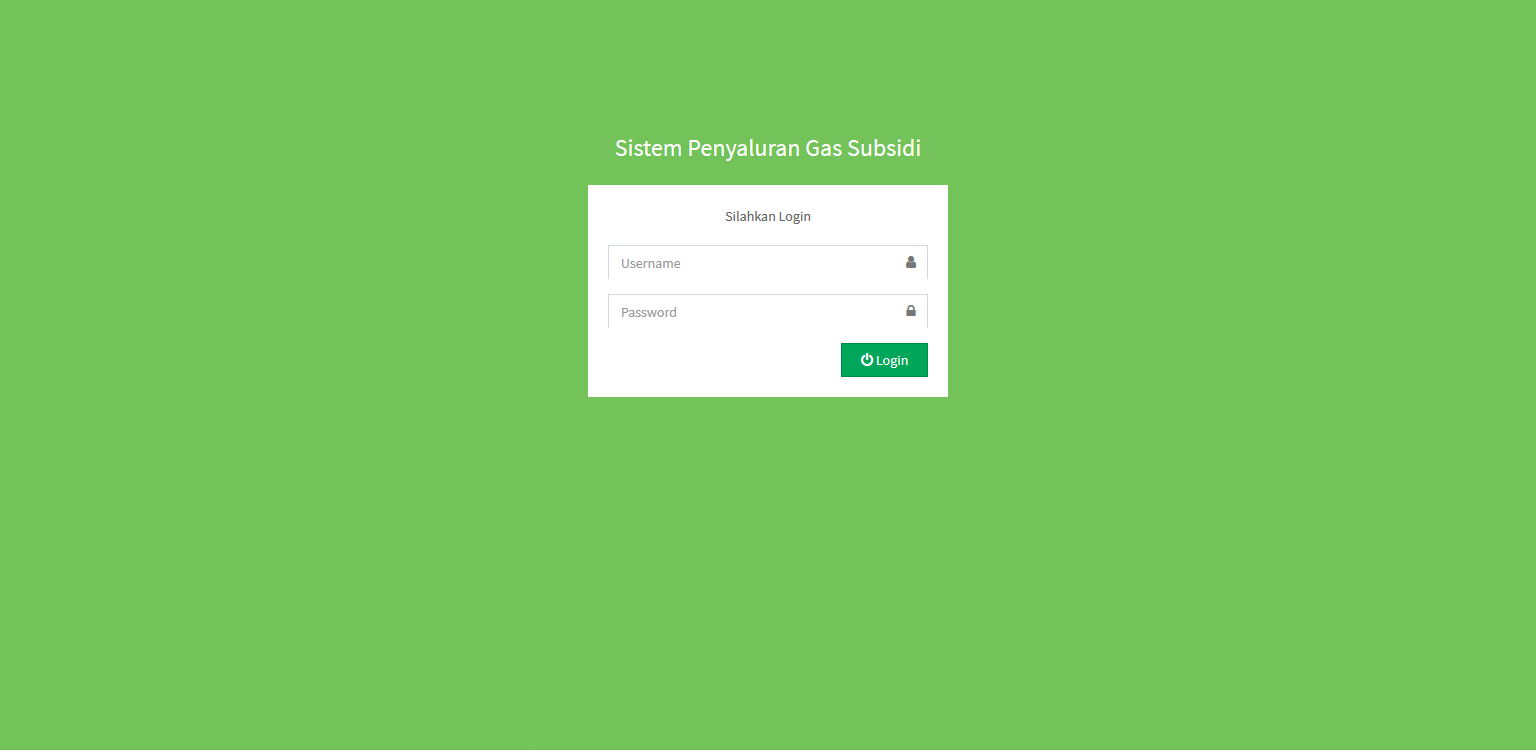
\includegraphics [width = 9cm]{gambar/web/login}
		\caption{Tampilan Halaman Login untuk Agen Gas LPG 3Kg}
		\label{tampilanLoginAgen}
	\end{figure}
	
	\begin{figure}[H]
		\center
		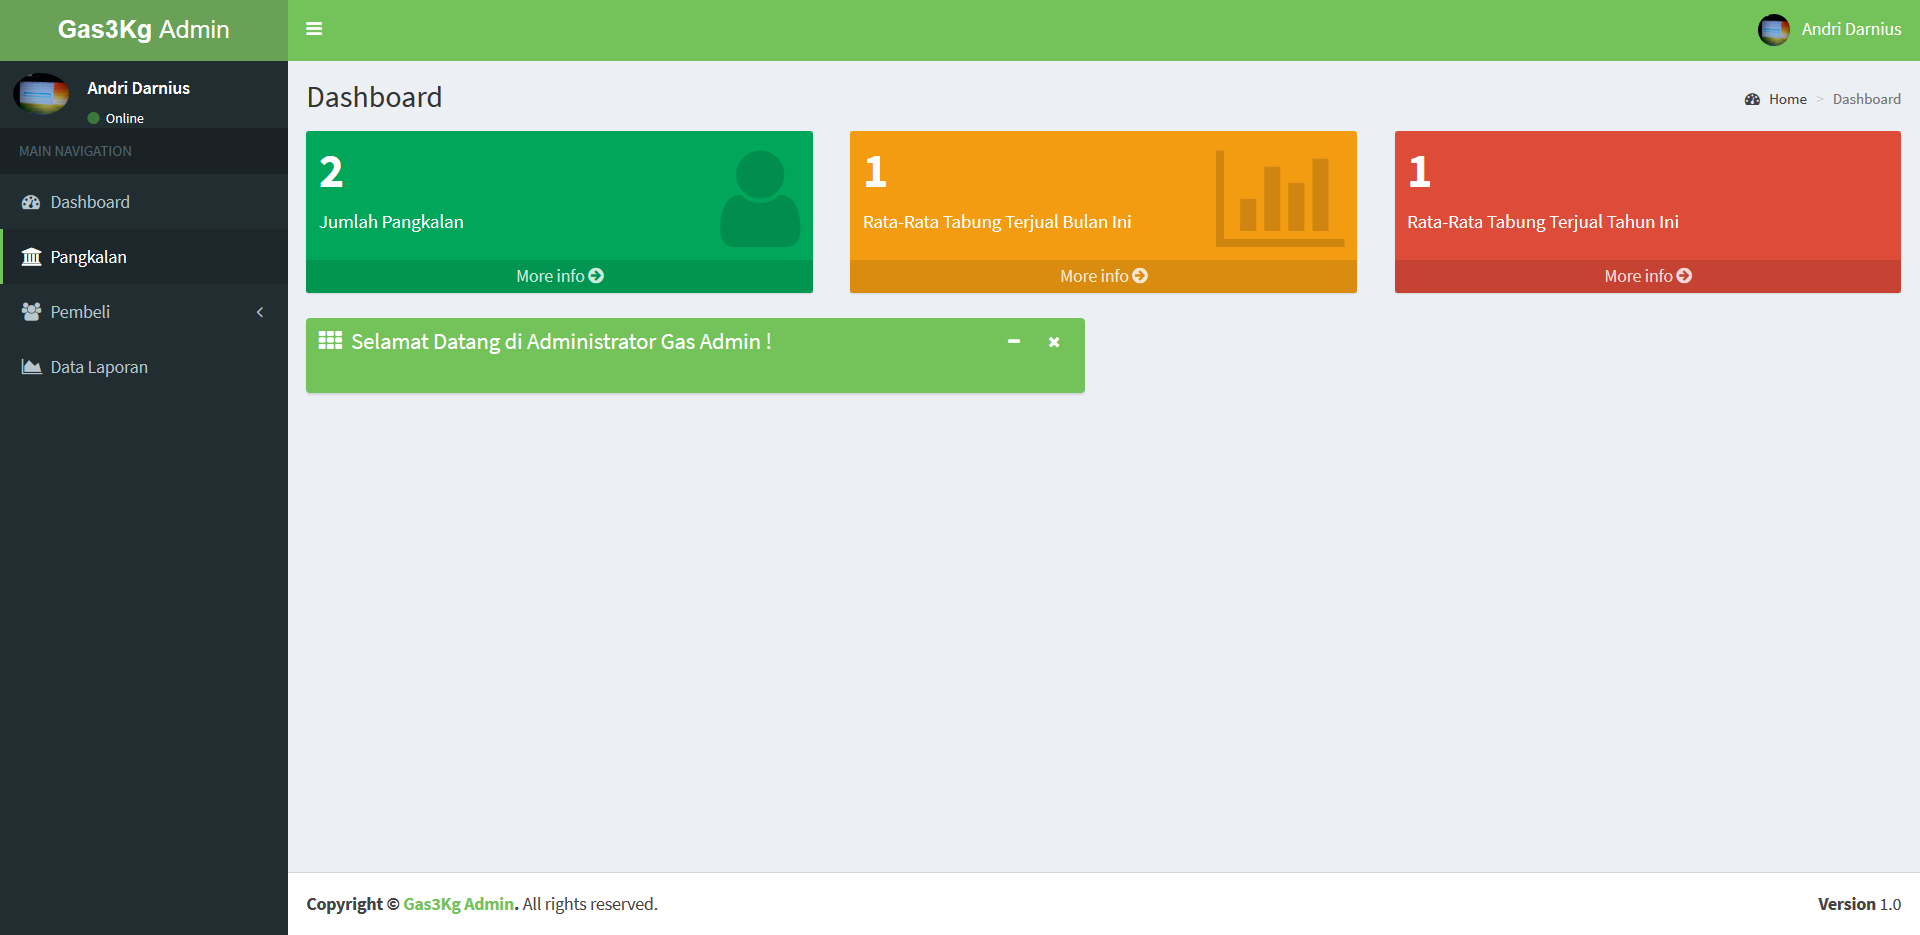
\includegraphics [width = 9cm]{gambar/web/beranda}
		\caption{Tampilan Halaman Beranda untuk Agen Gas LPG 3Kg}
		\label{tampilanBerandaAgen}
	\end{figure}

	\begin{figure}[H]
		\center
		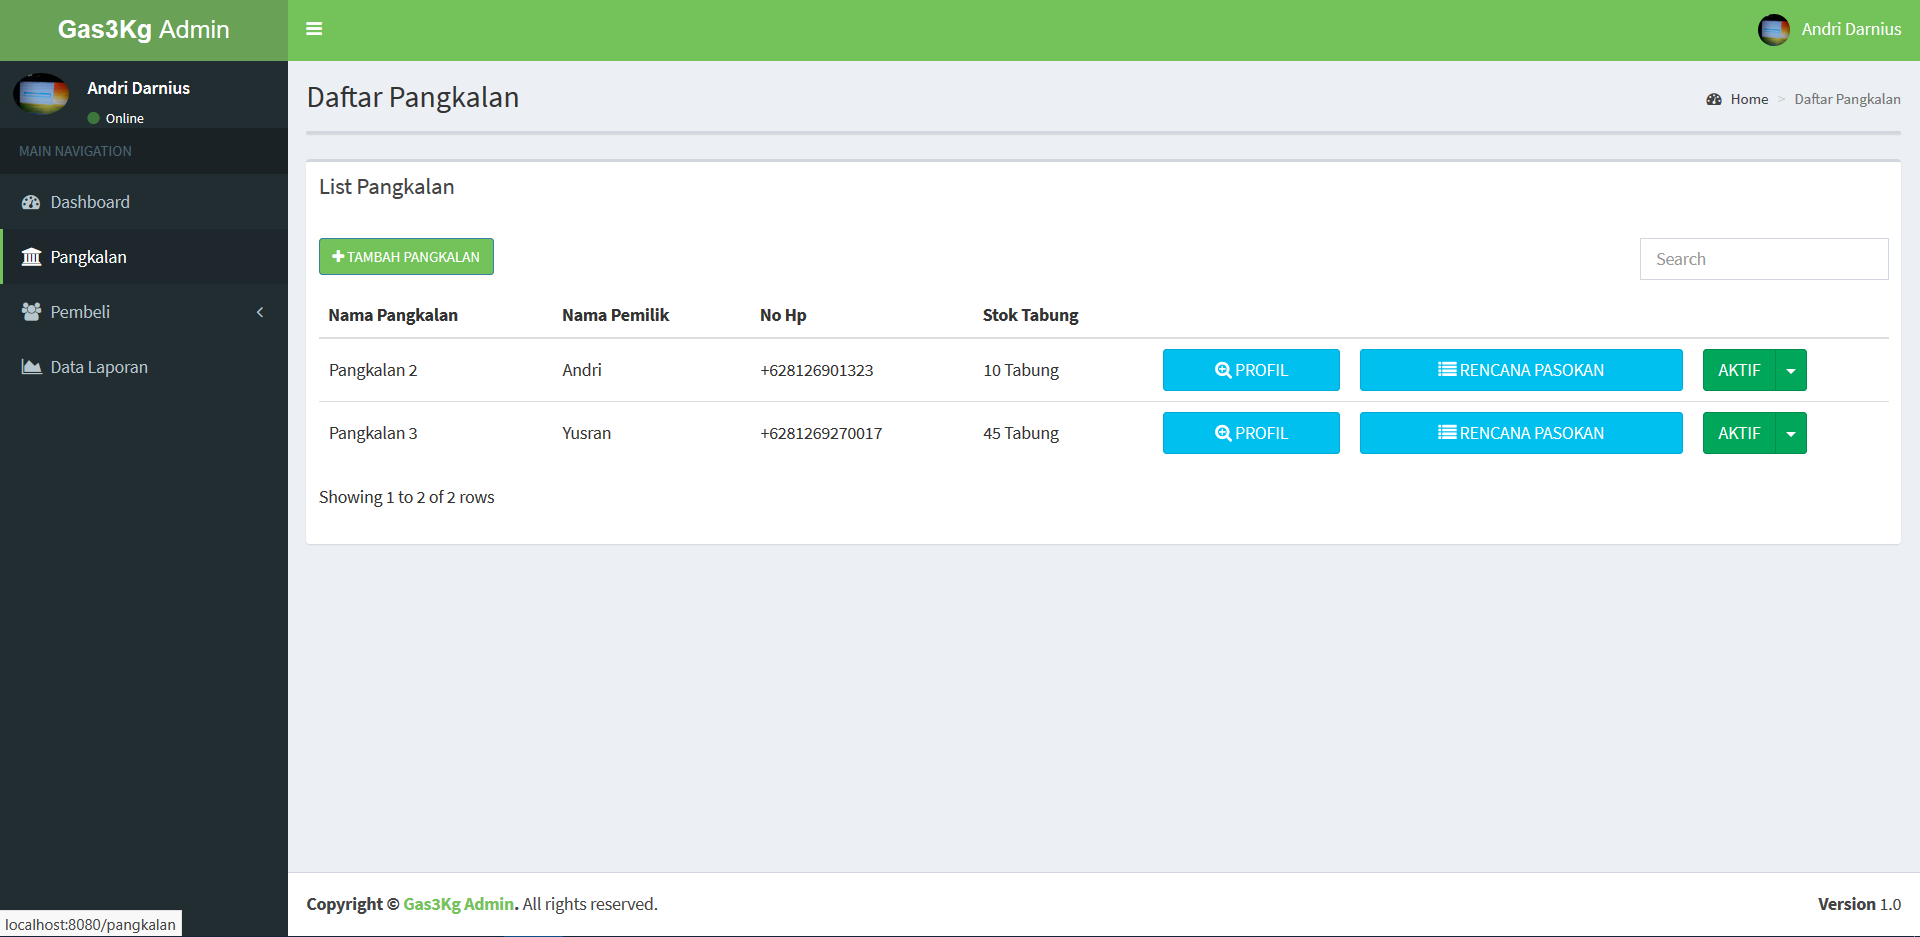
\includegraphics [width = 9cm]{gambar/web/pangkalan}
		\caption{Tampilan Halaman Daftar Pangkalan }
		\label{tampilanDaftarPangkalanAgen}
	\end{figure}

	\begin{figure}[H]
		\center
		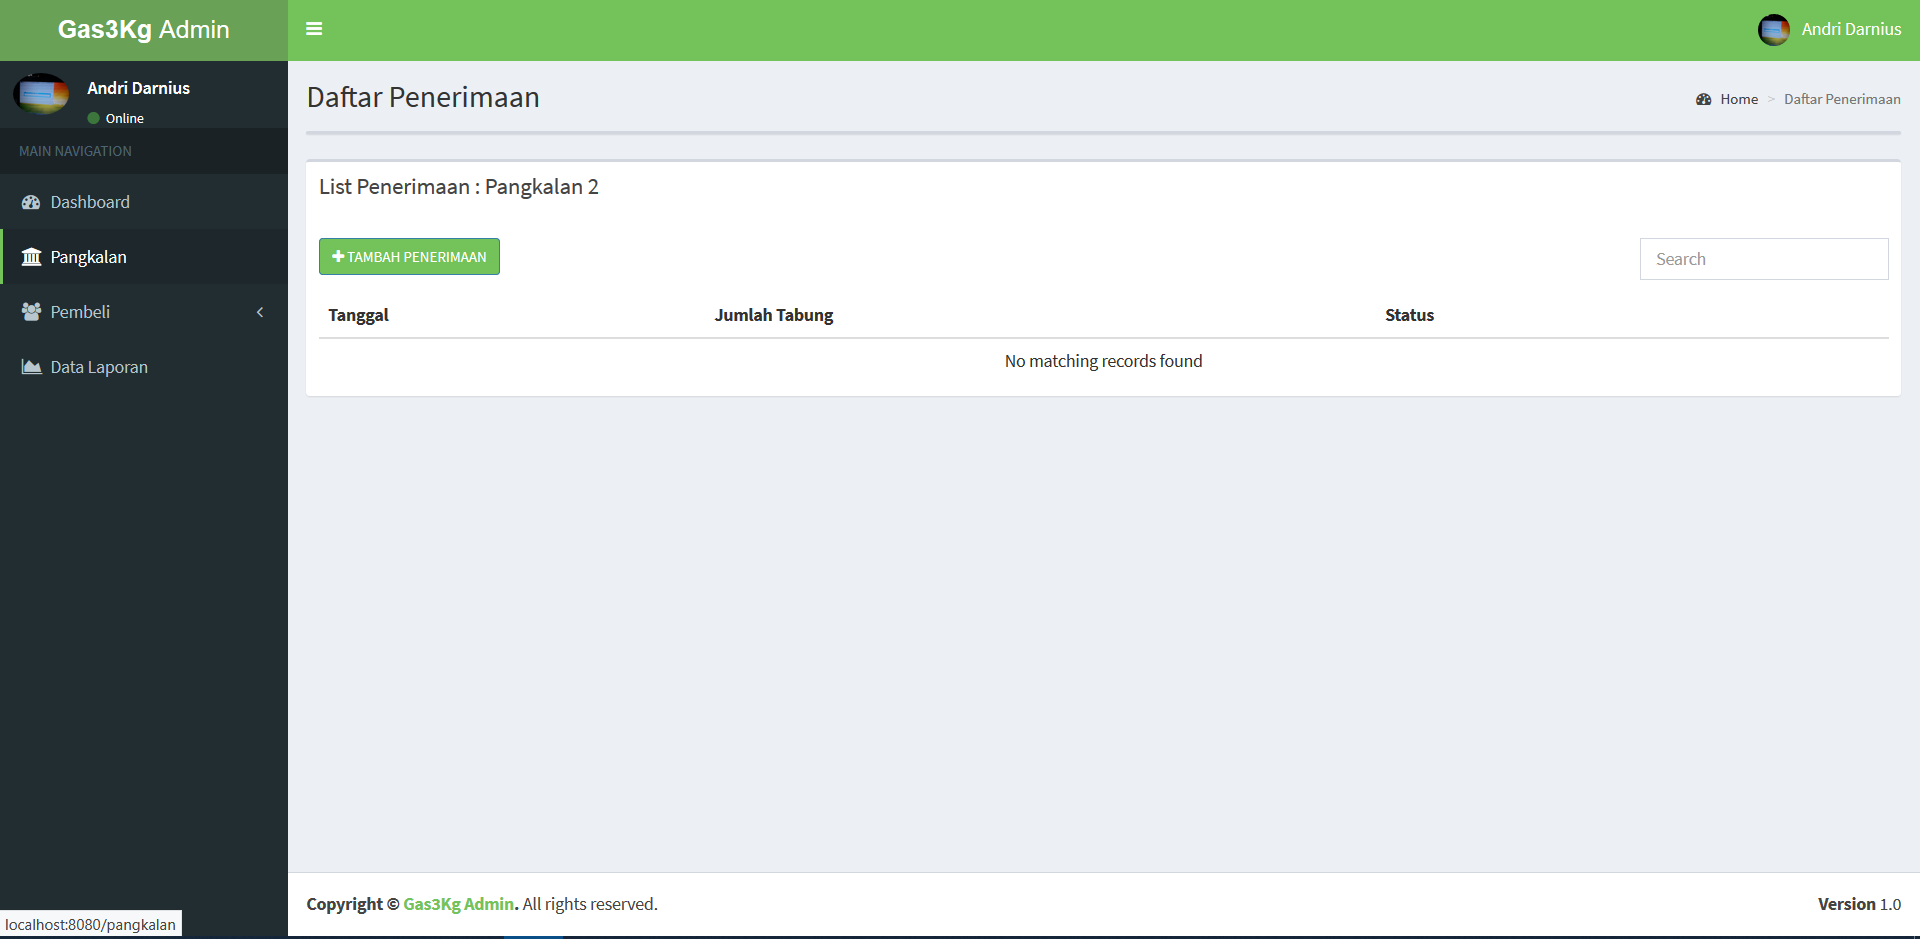
\includegraphics [width = 9cm]{gambar/web/penerimaan}
		\caption{Tampilan Halaman Rencana Penerimaan Pasokan Tabung}
		\label{tampilanPenerimaanAgen}
	\end{figure}

	\begin{figure}[H]
		\center
		\includegraphics [width = 9cm]{gambar/web/Laporan}
		\caption{Tampilan Halaman Ekspor Laporan}
		\label{tampilanLaporanAgen}
	\end{figure}
	
	
	
	\subsection{Pembuatan Sistem}
	
	\begin{enumerate}[a.]
		\item Layanan Web
		\\ Layanan web dikembangkan menggunakan bahasa pemrograman java dengan memanfaatkan pustaka Google Endpoints API untuk membangun sebuah layanan web yang memiliki prinsip RESTful API. dan juga menggunakan Google Datastore sebagai media penyimpanan basis data. Google Datastore merupakan layanan basis data NoSQL yang dibuat untuk penskalaan otomatis, kinerja tinggi, dan kemudahan dalam pengembangan aplikasi. Dikarenakan kita menggunakan Google Datastore sebagai Layanan penyimpanan basis data, kita akan menggunakan salah satu pustaka Java yang dimilikinya yaitu Objectify. Pada pembuatan layanan web (\textit{webservice}) hanya membutuhkan \textit{Model} Basis Data, \textit{Controller}, dan API. Pada pembuatan \textit{Model} basis data, desain basis datanya akan mengikuti dari desain \textit{class diagram} yang dibuat sebelumnya. tahap pembuatan layanan web yang pertama adalah membuat kelas \textit{Model} untuk masing-masing entitas seperti pada Gambar \ref{modelWebservice}. Setelah itu membuat kelas \textit{controller} yang akan menangani setiap operasi untuk memanipulasi data didalam \textit{Model} seperti pada Gambar \ref{controllerWebservice}. Tahap selanjutnya adalah membuat kelas API yang akan menangani pemanggilan setiap \textit{endpoint} yang layanan web seperti pada Gambar \ref{apiWebservice}. Setelah semua komponen telah selesai, maka akan dilakukan pengujian terhadap layanan web untuk mengetahui apakah setiap endpoint berjalan dengan seharusnya seperti pada Gambar \ref{pengujianApi}.
		
		\vspace{-0.4cm}
		\begin{figure}[H]
			\center
			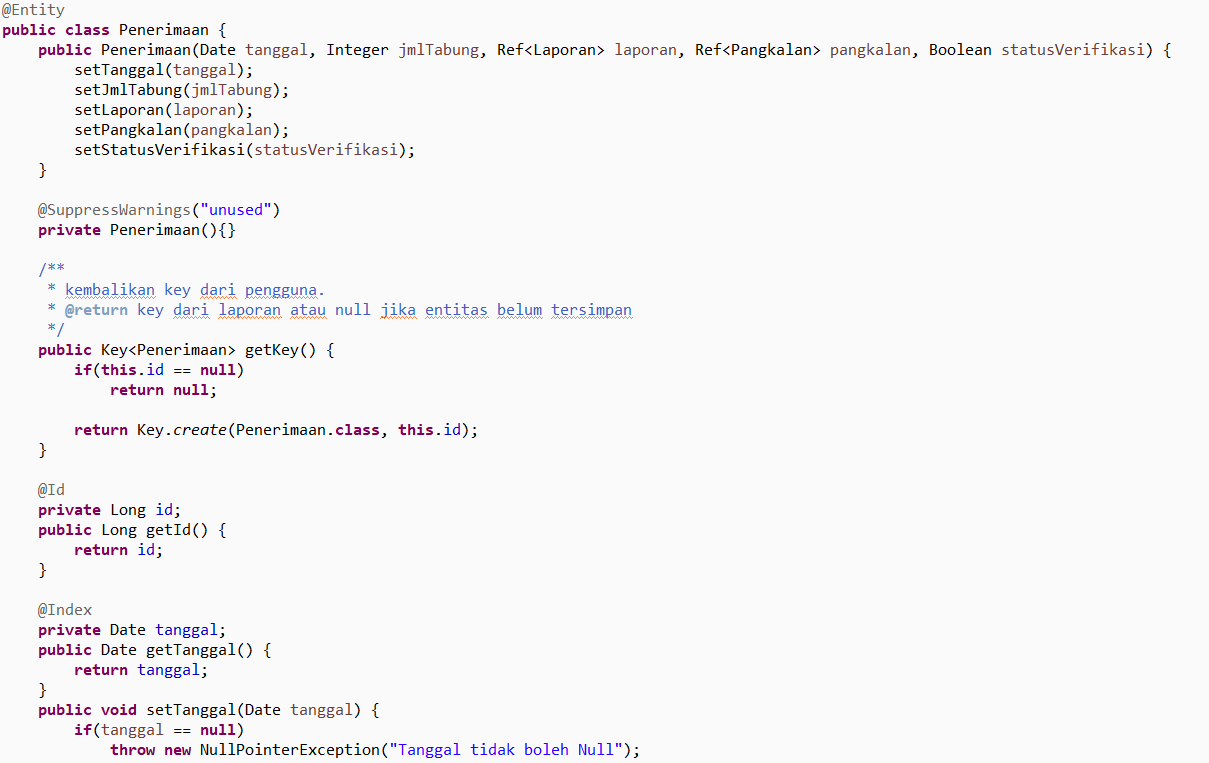
\includegraphics [width = 12cm]{gambar/kode/model-webservice}
			\caption{Potongan kode \textit{model} basis data layanan web}
			\label{modelWebservice}
		\end{figure}
	
		\begin{figure}[H]
			\center
			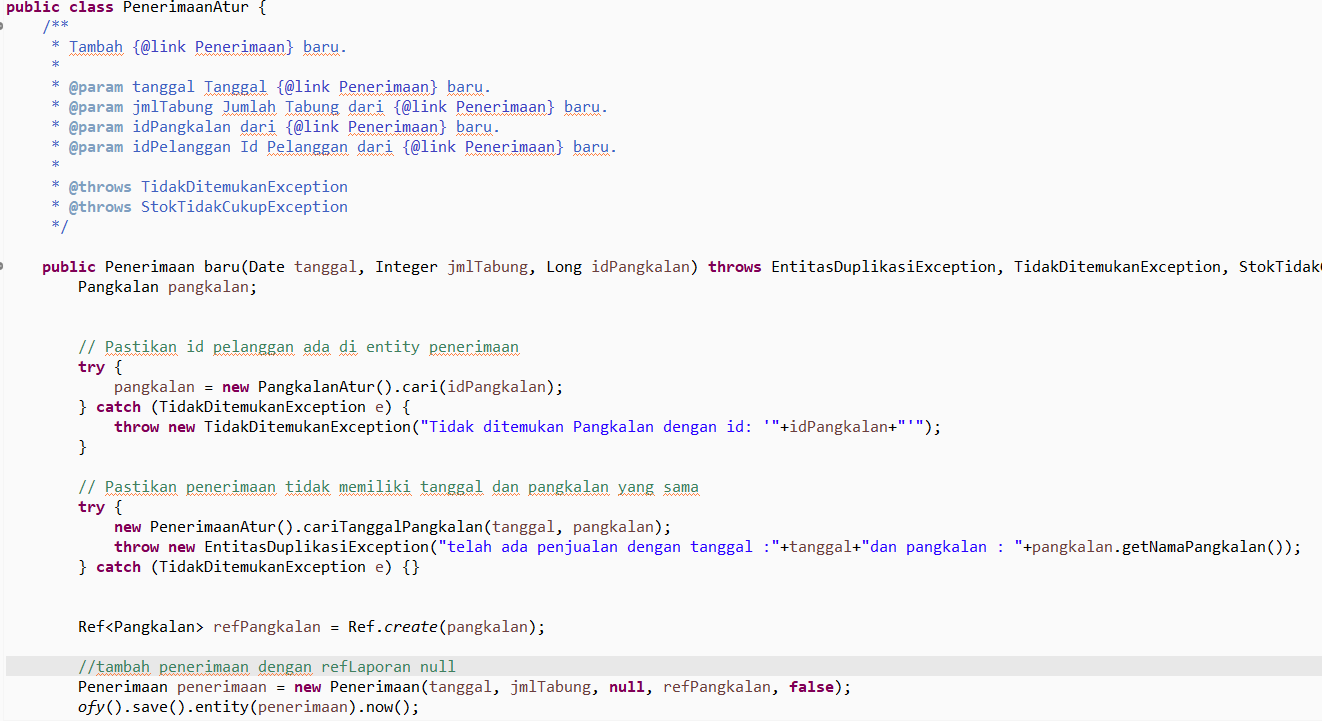
\includegraphics [width = 12cm]{gambar/kode/controller-webservice}
			\caption{Potongan kode \textit{controller} layanan web}
			\label{controllerWebservice}
		\end{figure}
	
		\begin{figure}[H]
			\center
			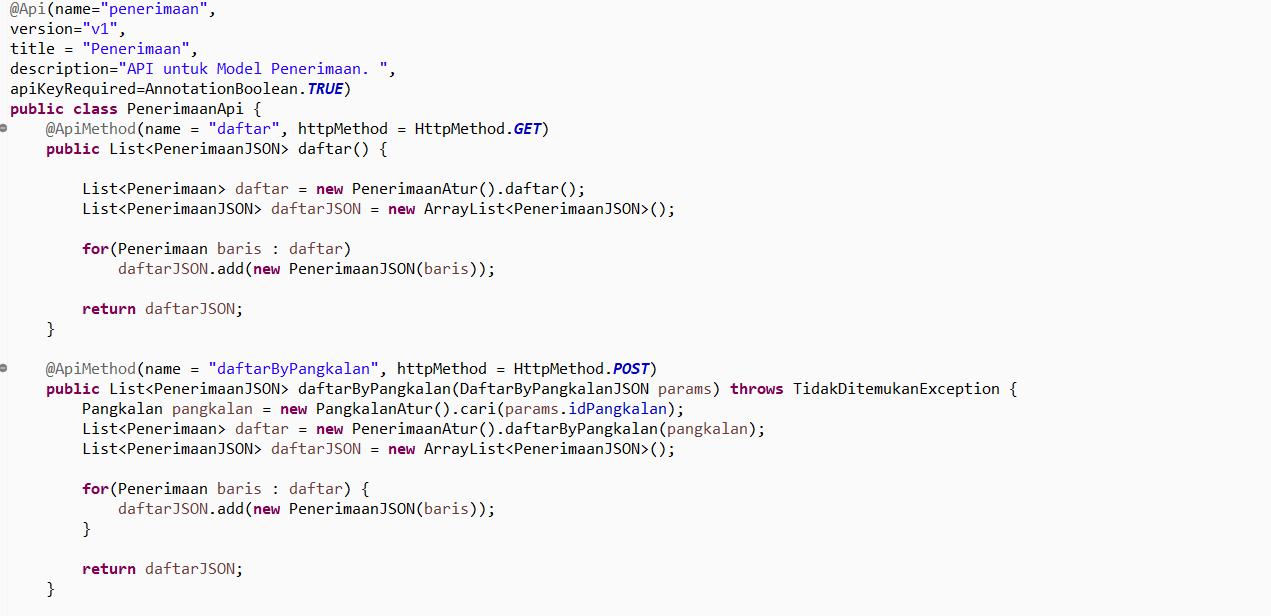
\includegraphics [width = 12cm]{gambar/kode/api-webservice}
			\caption{Potongan kode API layanan web}
			\label{apiWebservice}
		\end{figure}
	
		\begin{figure}[H]
			\center
			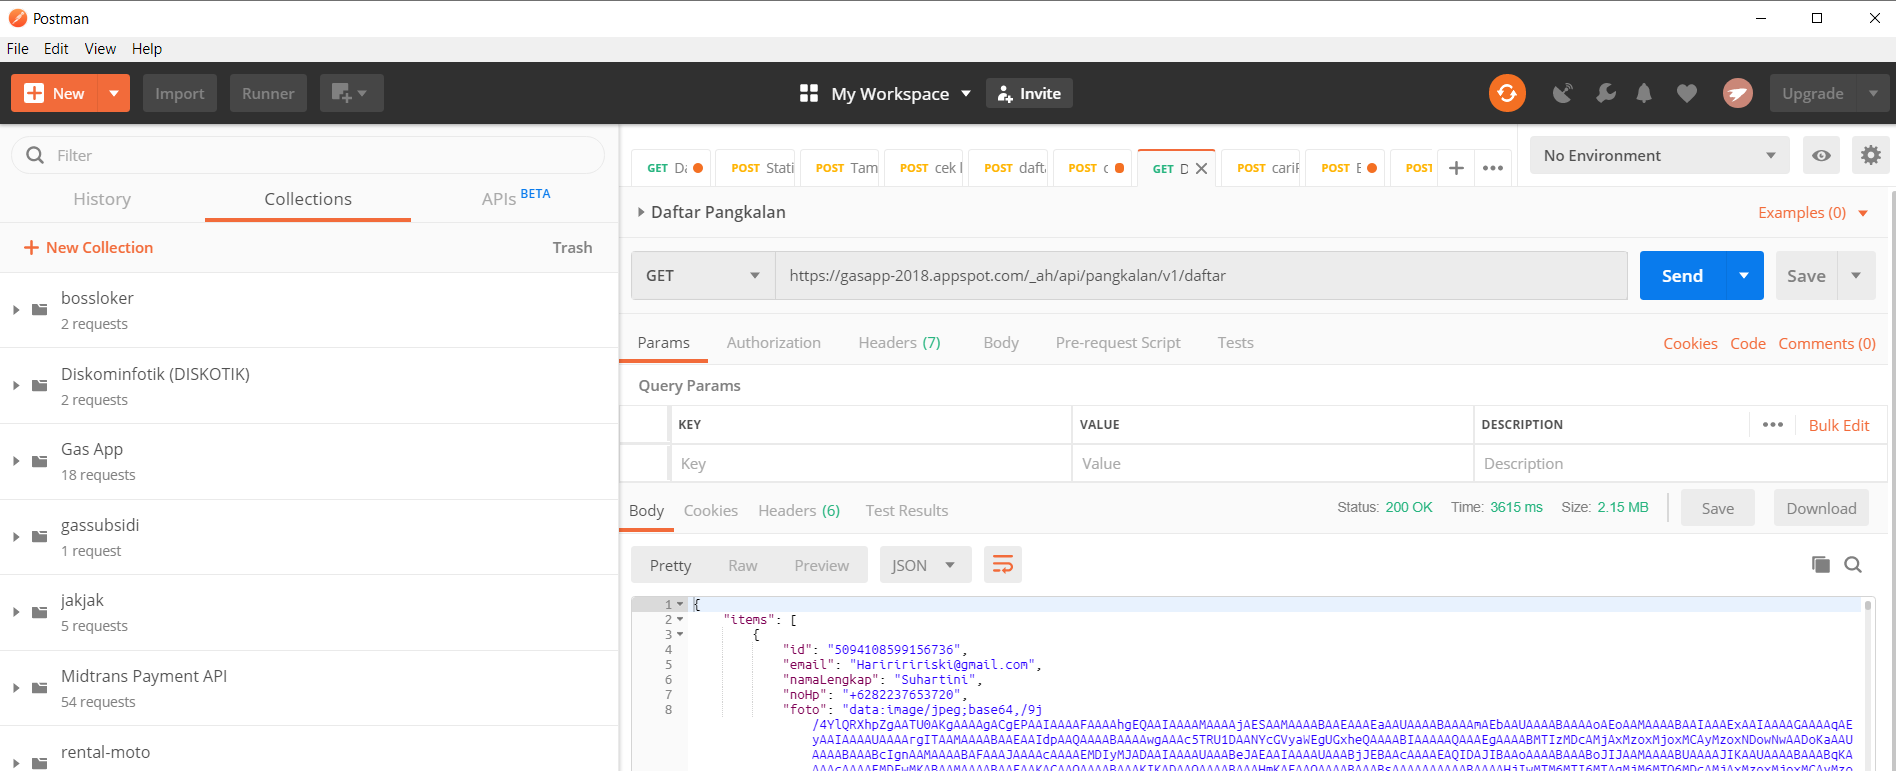
\includegraphics [width = 12cm]{gambar/pengujianApi}
			\caption{Contoh Pengujian Endpoint API pada layanan web (\textit{Webservice})}
			\label{pengujianApi}
		\end{figure} 
		
		\item Aplikasi Mobile
		\\ Aplikasi berbasis \textit{android} dikembangkan menggunakan Ionic Framework yang menggunakan teknologi HTML, JavaScript dan CSS sebagai tampilan \textit{frontend} aplikasi. Pengembangan aplikasi ini mengikuti salah satu prinsip pembuatan aplikasi secara umum yaitu MVC (Model View Controller). Model (providers) berisi fungsi untuk masing-masing method HTTP yang dipanggil oleh aplikasi dari layanan web. \textit{Model} dibuat menggunakan Typescript. \textit{Model} berperan penting pada proses penarikan dan penginputan data ke Google Datastore. Contoh Kode model pada ionic dapat dilihat pada Gambar \ref{modelMobile}. \textit{View} berfungsi untuk mengatur tampilan aplikasi yang ditampilkan pada pengguna melalui HTML dan CSS. Contoh Kode view pada ionic dapat dilihat pada Gambar \ref{modelView}. \textit{Controller} untuk mengatur halaman yang ditampilkan kepada pengguna dan pemanggilan API. \\
		
		\vspace{-0.4cm}
		\begin{figure}[H]
			\center
			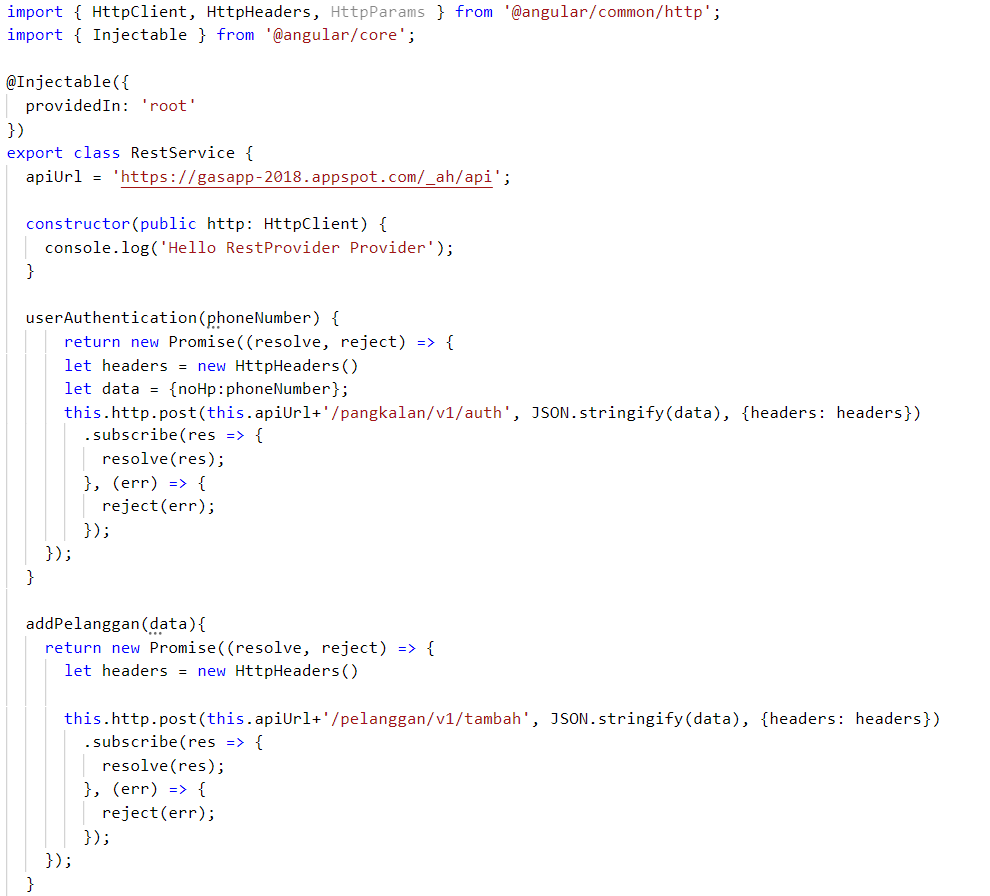
\includegraphics [width = 12cm]{gambar/kode/model-mobile}
			\caption{Potongan kode \textit{model} aplikasi berbasis android}
			\label{modelMobile}
		\end{figure}
		
		\begin{figure}[H]
			\center
			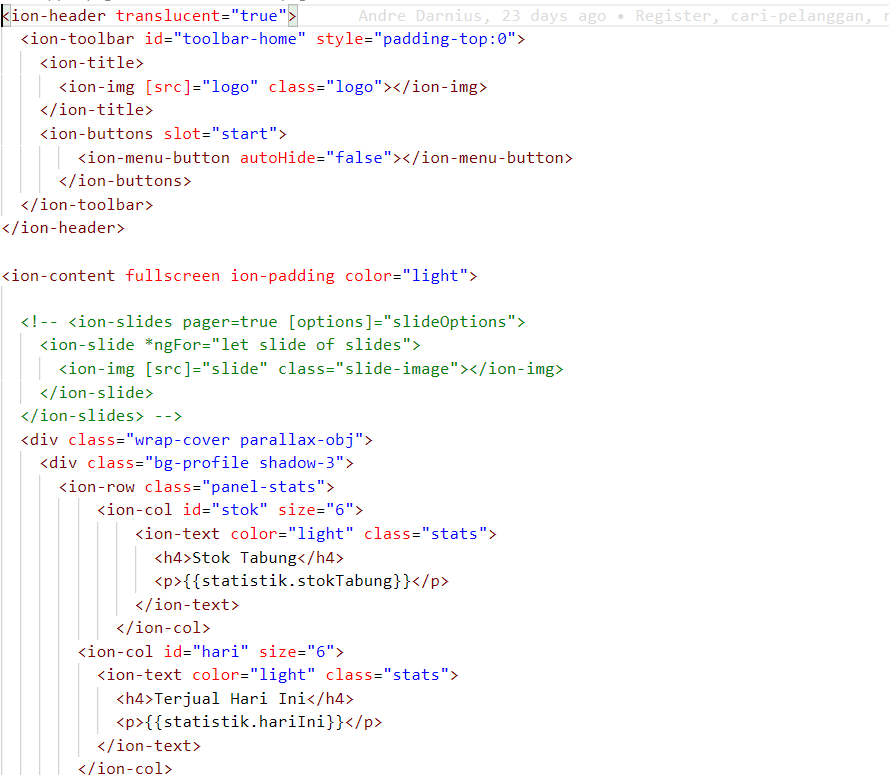
\includegraphics [width = 12cm]{gambar/kode/view-mobile}
			\caption{Potongan kode \textit{view} aplikasi berbasis android}
			\label{viewMobile}
		\end{figure}
		
		\begin{figure}[H]
			\center
			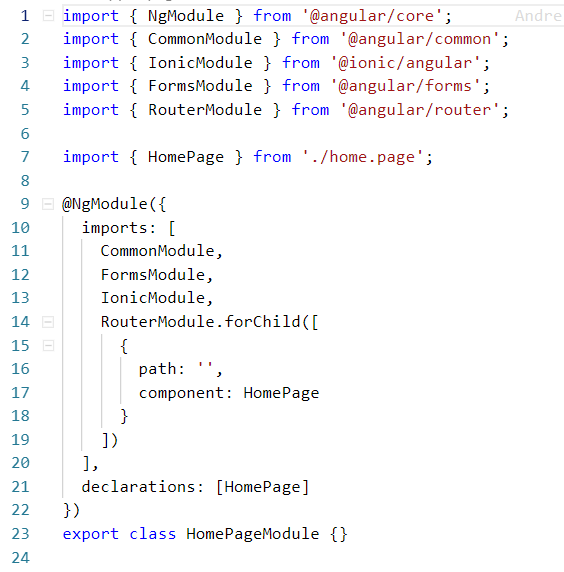
\includegraphics [width = 12cm]{gambar/kode/controller-mobile}
			\caption{Potongan kode \textit{controller} aplikasi berbasis android}
			\label{controllerMobile}
		\end{figure}
		
		 aplikasi ini juga menggunakan layanan Google Firebase untuk dapat melakukan proses login menggunakan nomor HP atau dinamakan dengan \textit{Phone Authentication} seperti pada Gambar \ref{firebaseAuth}
		
		\begin{figure}[H]
			\center
			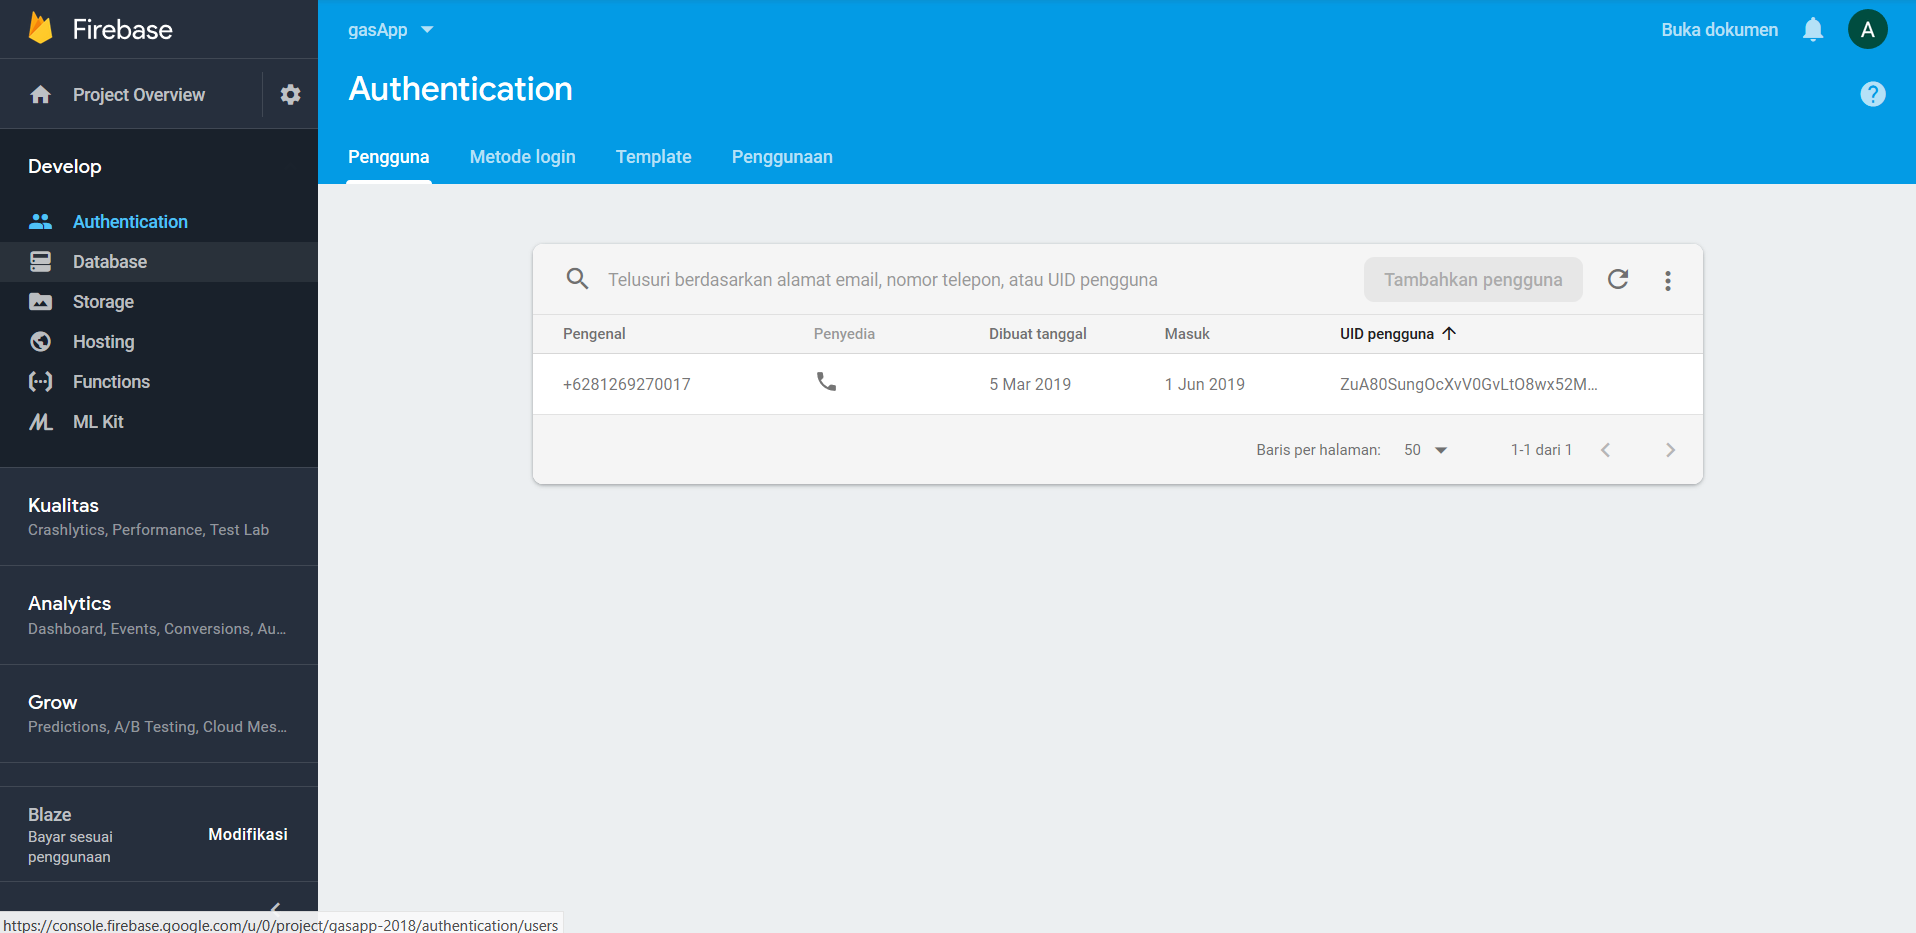
\includegraphics [width = 12cm]{gambar/firebaseAuth}
			\caption{Halaman Konsole  \textit{Phone Authentication} pada Google Firebase}
			\label{firebaseAuth}
		\end{figure} 
	
		\pagebreak
		
		\item Aplikasi Web
		\\ Aplikasi berbasis \textit{web} dikembangkan menggunakan Bahasa pemrograman Java dengan menggunakan prinsip yang sama yaitu MVC (Model View Controller). dimana \textit{model} menggunakan pustaka HTTP untuk memanggil method HTTP pada layanan web dan pustaka GSON untuk melakukan proses konversi dari JSON ke dalam objek java. untuk \textit{view} menggunakan JSP (\textit{Java Server Page}) untuk menampilkan isi halaman \textit{web} yang akan dibangun. JSP memiliki struktur bahasa yang hampir sama dengan HTML (\textit{Hypertext Markup Language}). untuk \textit{controller} menggunakan pustaka HTTP Servlet untuk menangani permintaan HTTP URL dan mengatur pemanggilan \textit{view dan model}. Aplikasi ini nanti akan berjalan pada platform Google App Engine (GAE)\\
		
		\vspace{-0.4cm}
		\begin{figure}[H]
			\center
			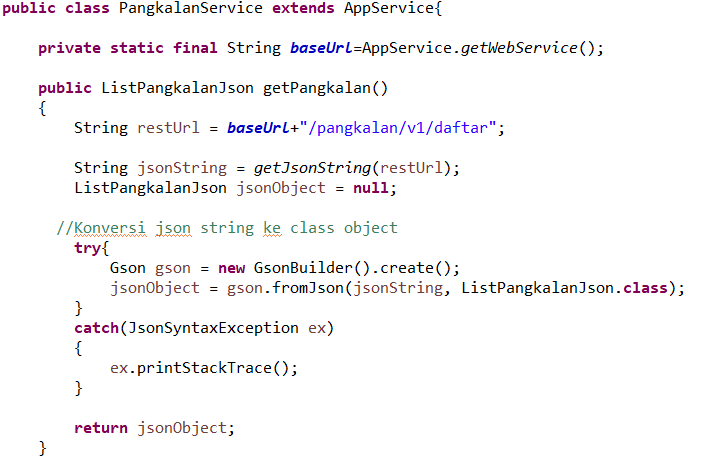
\includegraphics [width = 14cm]{gambar/kode/model-web}
			\caption{Potongan kode \textit{model} aplikasi berbasis web}
			\label{modelWeb}
		\end{figure}
		
		\begin{figure}[H]
			\center
			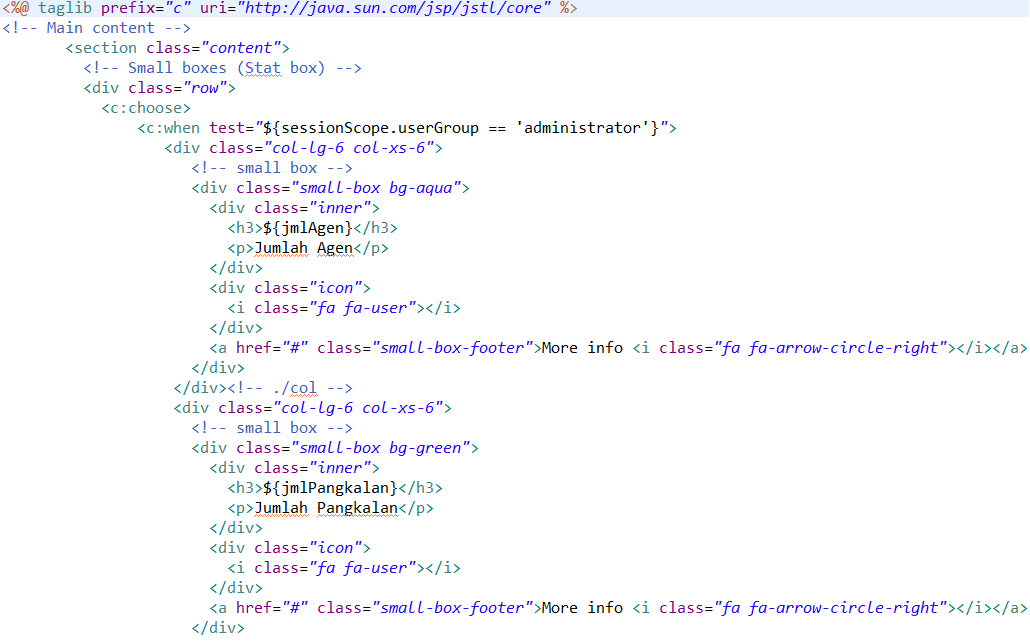
\includegraphics [width = 15cm]{gambar/kode/view-web}
			\caption{Potongan kode \textit{view} aplikasi berbasis web}
			\label{viewWeb}
		\end{figure}
		
		\begin{figure}[H]
			\center
			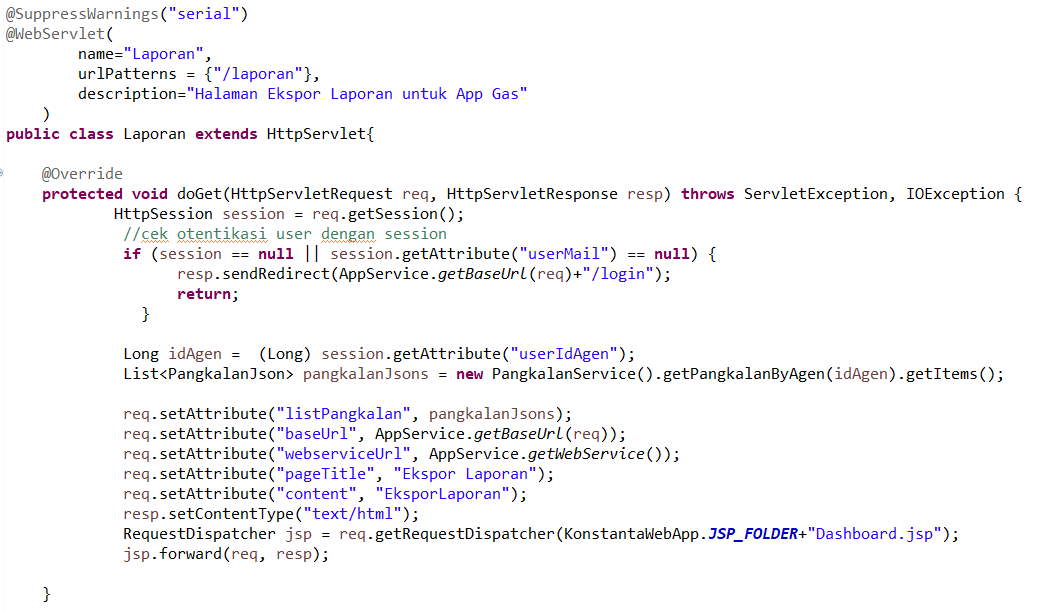
\includegraphics [width = 14cm]{gambar/kode/controller-web}
			\caption{Potongan kode \textit{controller} aplikasi berbasis web}
			\label{controllerWeb}
		\end{figure}
	
		Aplikasi berbasis web ini menggunakan layanan Google Sign-in untuk melakukan proses login dengan memakai email google sebagai ID Pengenal. Untuk proses implementasinya hanya dengan menanamkan \textit{script} javascript pada halaman login seperti pada Gambar \ref{loginWeb}. Aplikasi ini juga memakai pustaka java yang bernama itext untuk melakukan ekspor data penyaluran tabung dalam bentuk \textit{file} PDF. Berikut potongan kode untuk melakukan proses ekspor pada Gambar \ref{eksporWeb}.
	
		\begin{figure}[H]
			\center
			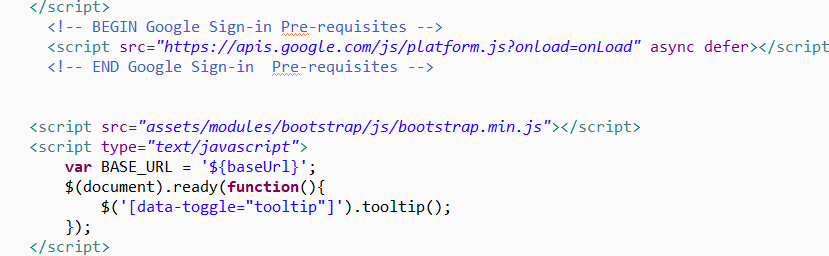
\includegraphics [width = 14cm]{gambar/kode/login-web}
			\caption{Potongan kode Login memakai email aplikasi berbasis web}
			\label{loginWeb}
		\end{figure}
	
		\begin{figure}[H]
			\center
			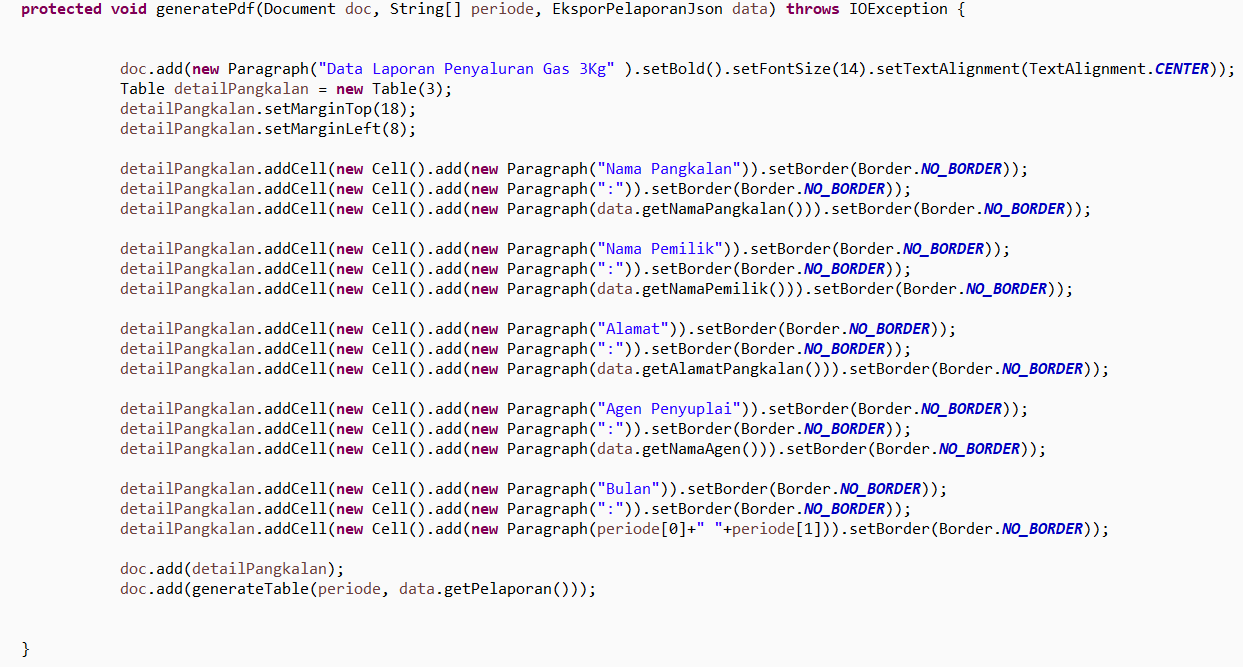
\includegraphics [width = 14cm]{gambar/kode/ekspor-web}
			\caption{Potongan kode ekspor data aplikasi berbasis web}
			\label{eksporWeb}
		\end{figure}

	\end{enumerate}

	
	\section{Pengujian Sistem}
	
		\subsection{Metode \textit{Whitebox}}
			\par Pada pengujian \textit{whitebox}, aplikasi ini menggunakan JUnit yang dapat melakukan pengujian secara otomatis. Aspek-aspek yang diuji pada pengujian ini adalah bagaimana program yang dibangun bukan hanya dapat berjalan dengan semestinya (\textit{test success}), tapi pada saat diberikan sebuah parameter yang salah program dapat mengembalikan error yang semestinya (\textit{test fail}). Aplikasi yang dibangun telah dianggap lulus pengujian apabila mampu melewati semua \textit{test} secara sempurna 100\%. 
			
			\begin{figure}[H]
				\center
				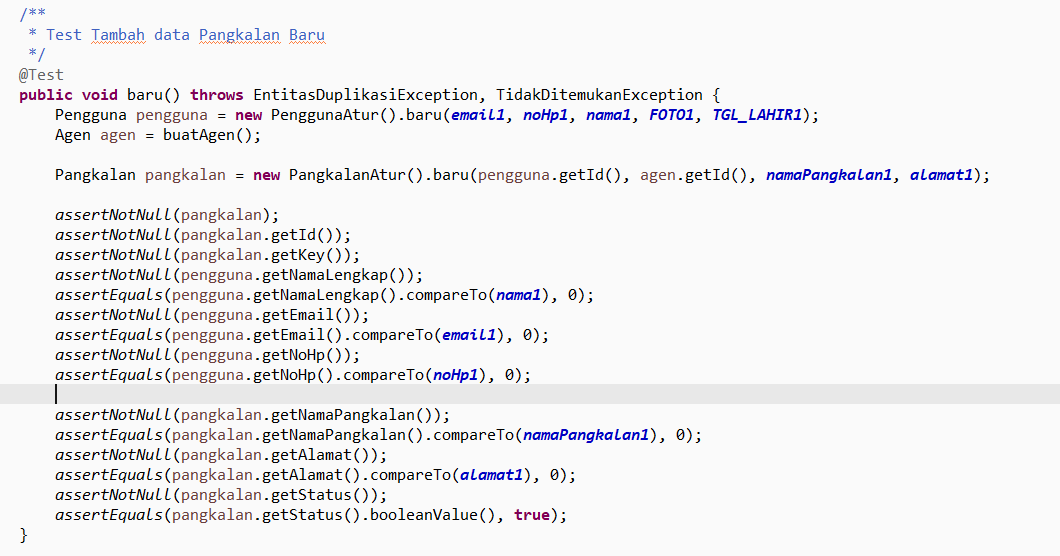
\includegraphics [width = 14cm]{gambar/kode/test-success}
				\caption{Potongan kode Pengujian JUnit dengan kasus berhasil (\textit{test success})}
				\label{testSuccess}
			\end{figure}
		
			\begin{figure}[H]
				\center
				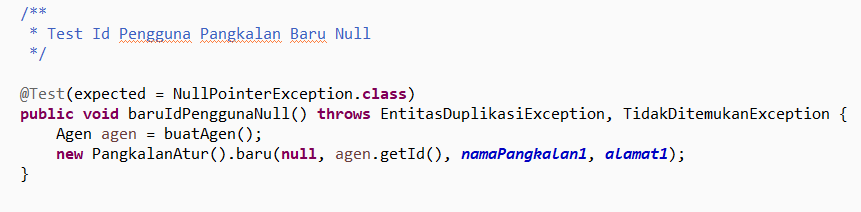
\includegraphics [width = 14cm]{gambar/kode/test-fail}
				\caption{Potongan kode Pengujian JUnit dengan kasus gagal (\textit{test fail})}
				\label{testFail}
			\end{figure}
		
			\begin{figure}[H]
				\center
				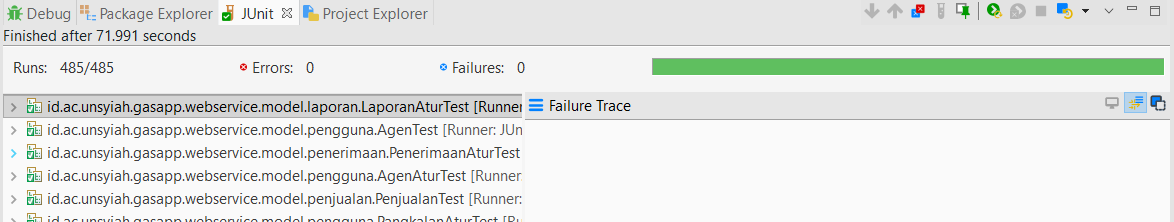
\includegraphics [width = 14cm]{gambar/kode/junit-success}
				\caption{Pengujian JUnit Berhasil}
				\label{junitSuccess}
			\end{figure}
		
			\begin{figure}[H]
				\center
				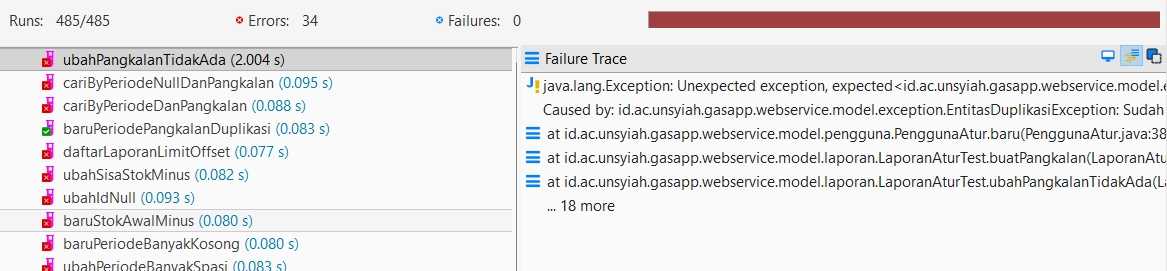
\includegraphics [width = 14cm]{gambar/kode/junit-fail}
				\caption{Pengujian JUnit Gagal}
				\label{junitFail}
			\end{figure}
	
	
	\subsection{Metode \textit{Blackbox}}
	
	Pada pengujian menggunakan metode \textit{blackbox}, aspek yang diuji adalah aspek fungsionalitas dari aplikasi tanpa melihat proses logika yang terjadi dibelakang. Berikut hasil dari pengujian ini dapat dilihat pada tabel \ref{ujiWeb} untuk aplikasi berbasis \textit{web} dan tabel \ref{ujiMobile} untuk aplikasi android.
	
	\begin{longtable}{ |c|p{3cm}|p{3cm}|p{3cm}|p{2cm}|}
	\caption{Pengujian \textit{blackbox} pada aplikasi berbasis web}
	\label{ujiWeb} \\ \hline
	\textbf{No.}                  &  \textbf{Nama Pengujian}         & \textbf{Skenario}                                       & \textbf{Luaran}              & \textbf{Hasil Pengujian} \\ \hline
	
	
	\multirow{2}{*}{1.}  & 	\multirow{2}{*}{Login Akun} & Klik \textit{link} "Login menggunakan Email Google"           & Tampil form login google yang harus diisi oleh pengguna.             & Berhasil \\ \cline{3-5}
	& & Masukkan email google dan passwordnya           & muncul halaman beranda         & Berhasil \\ \hline
	
	\multirow{3}{*}{2.}  & 	\multirow{3}{*}{Tambah Pangkalan} & Klik menu pangkalan           & Tampil daftar pangkalan yang ada.             & Berhasil \\ \cline{3-5}
	& & Klik tombol "tambah pangkalan"           & Tampil form untuk menginput data pangkalan baru.             & Berhasil \\ \cline{3-5}
	& & Masukkan data pangkalan ke dalam form dan klik tombol "simpan"           & Muncul peringatan bahwa pangkalan telah berhasil ditambah.             & Berhasil \\ \hline
	
	\multirow{4}{*}{3.}  & 	\multirow{4}{*}{Edit Pangkalan} & Klik menu pangkalan           & Tampil daftar pangkalan yang ada.             & Berhasil \\ \cline{3-5}
	& & Klik tombol "profil"           & Tampil form data pangkalan yang ter-\textit{disable} semua.             & Berhasil \\ \cline{3-5}
	& & Klik tombol "edit"           & form tadi dapat diedit             & Berhasil \\ \hline
	& & Edit data pangkalan pada form dan klik tombol "simpan"           & Muncul peringatan bahwa pangkalan telah berhasil diedit.             & Berhasil \\ \hline
	
	
	\multirow{4}{*}{4.}  & 	\multirow{4}{*}{\parbox{3cm}{\centering Tambah Rencana Pasokan Tabung}} & Klik menu pangkalan           & Tampil daftar pangkalan yang ada.             & Berhasil \\ \cline{3-5}
	& & Klik tombol "Rencana Pasokan"           & Tampil halaman daftar pasokan tabung untuk pangkalan tersebut.             & Berhasil \\ \cline{3-5}
	& & Klik tombol "tambah penerimaan"           & Muncul form untuk menginput data rencana pasokan.             & Berhasil \\ \cline{3-5}
	& & Masukkan data pasokan tabung ke dalam form dan klik tombol "simpan"     & Muncul peringatan bahwa data pasokan telah berhasil ditambah.             & Berhasil \\ \hline
	
	\multirow{2}{*}{5.}  & 	\multirow{2}{*}{Ekspor Laporan} & Klik menu data laporan          & Tampil Form Ekspor Laporan.             & Berhasil \\ \cline{3-5}
	& & Masukkan periode laporan dan milik pangkalan mana setelah itu klik tombol "Ekspor Data"     & Muncul laporan penyaluran tabung dalam bentuk file PDF.             & Berhasil \\ \hline
		
	\end{longtable}

	\pagebreak
	
	\begin{longtable}{ |c|p{3cm}|p{3cm}|p{3cm}|p{2cm}|}
		\caption{Pengujian \textit{blackbox} pada aplikasi berbasis android}
		\label{ujiMobile} \\ \hline
		\textbf{No.}                  &  \textbf{Nama Pengujian}         & \textbf{Skenario}                                       & \textbf{Luaran}              & \textbf{Hasil Pengujian} \\ \hline
		
		
		\multirow{2}{*}{1.}  & 	\multirow{2}{*}{Login Akun} & Masukkan no HP akun pangkalan yang telah terdaftar           & masuk SMS kode OTP dan  Tampil halaman verifikasi OTP         & Berhasil \\ \cline{3-5}
		& & Masukkan Kode OTP dan tekan tombol "verifikasi"           & muncul halaman beranda         & Berhasil \\ \hline
		\multirow{5}{*}{2.}  & 	\multirow{5}{*}{\parbox{3cm}{\centering Register Pelanggan}} & Klik menu "register pelanggan"           & Tampil form untuk menginput data pelanggan            & Berhasil \\ \cline{3-5}
		& & Masukkan data pelanggan ke dalam form dan klik tombol "simpan"           & Tampil halaman untuk mengupload berkas pelanggan.             & Berhasil \\ \cline{3-5}
		& &  Tekan tombol "foto diri" untuk mengambil foto diri pelanggan        & Tombol "foto diri" akan terdapat logo centang             & Berhasil \\ \cline{3-5}
		& &  Tekan tombol "foto KTP" untuk mengambil foto ktp pelanggan        & Tombol "foto KTP" akan terdapat logo centang             & Berhasil \\ \cline{3-5}
		& &  Tekan tombol "simpan" untuk menginput data pelanggan baru   & Muncul peringatan bahwa data pelanggan baru telah berhasil ditambah.             & Berhasil \\ \hline
		
		\multirow{1}{*}{3.}  & 	\multirow{1}{*}{Penjualan Tabung} & Klik menu "Penjualan Tabung"          & Tampil halaman untuk mencari pelanggan.             & Berhasil \\ \hline
		\multirow{5}{*}{} & \multirow{5}{*}{} & Masukkan nik dari pelanggan yang membeli tabung dan tekan nama pelanggan           & Tampil data detail pelanggan.             & Berhasil \\ \cline{3-5}
		& & Klik tombol "beli tabung"           & tampil halaman pilihan jumlah tabung & Berhasil
		 \\ \cline{3-5}
		& & tekan salah pilihan tabung           & Tampil halaman untuk mengupload bukti pembelian.             & Berhasil \\ \cline{3-5}
		& &  Tekan tombol "foto Bukti Pembelian" untuk mengambil foto Bukti Pembelian pelanggan        & Tombol "foto Bukti Pembelian" akan terdapat logo centang             & Berhasil \\ \cline{3-5}
		& &  Tekan tombol "simpan" untuk menginput data penjualan  & Muncul peringatan bahwa penjualan baru telah berhasil.             & Berhasil \\ \hline
		
		\multirow{4}{*}{4.}  & 	\multirow{4}{*}{\parbox{3cm}{\centering Riwayat Pembelian Tabung}} & Klik menu "Penjualan Tabung"          & Tampil halaman untuk mencari pelanggan.             & Berhasil \\ \cline{3-5}
		 & & Masukkan nik dari pelanggan yang membeli tabung dan tekan nama pelanggan           & Tampil data detail pelanggan.             & Berhasil \\ \cline{3-5}
		& & Tekan tombol "riwayat pembelian"           & tampil halaman daftar riwayat pembelian tabung & Berhasil
		\\ \hline
		& & tekan salah satu dari daftar pembelian           & Tampil halaman yang menampilkan foto bukti pembelian.             & Berhasil \\ \hline
	
		
		
		\multirow{3}{*}{5.}  & 	\multirow{3}{*}{\parbox{3cm}{\centering Verifikasi Penerimaan Pasokan Tabung}} & Klik menu "Penerimaan Tabung"           & Tampil daftar penerimaan pasokan yang ada.             & Berhasil \\ \cline{3-5}
		& & geser salah salah satu daftar penerimaan dan tekan tombol centang           & Tampil peringatan konfirmasi penerimaan tabung.             & Berhasil \\ \cline{3-5}
		& & Tekan tombol "ya"           & Muncul peringatan bahwa penerimaan tabung telah berhasil dan jumlah tabung bertambah.             & Berhasil \\ \hline
		
	\end{longtable}

	Berdasarkan tabel \ref{ujiWeb} dan tabel \ref{ujiMobile} seluruh pengujian yang telah dilakukan berhasil sehingga aplikasi web dan android sudah dapat berjalan dengan baik. 
	
	\subsection{Metode \textit{Usability Testing}}
	
	Setelah melakukan pengujian sistem, selanjutnya aplikasi akan diuji dengan pengujian \textit{Usability Testing} pada tujuh responden dan mengisi kuesioner SUS. SUS memiliki kuesioner yang terdiri dari 10 pertanyaan. Contoh dari SUS dapat dilihat pada tabel \ref{kuesioner}. \textit{Test Plan} pengujian ini dapat dilihat pada tabel \ref{test plan}.
	
		\begin{center}
		\begin{table}[H]
			\center
			\caption{\textit{Test Plan }pengujian \textit{usability} aplikasi}
			\label{test plan}
			\begin{tabular}{ |p{12cm}|  }
				\hline
				\multicolumn{1}{|c|}{\textbf{\textit{Test Plan} \textit{Usablity Testing}}} \\
				\hline
				Lokasi :
				\begin{enumerate}
					\item PT Pasha Jaya, Meuraxa
					\item Starjazz Kupi, Batoh
					\item Dhapu Kupi, Batoh
					\item Pangkalan Gas Ateuk Meunjeng
					\item Pangkalan Gas Lingke
					\item Pangkalan Gas Lampeunereut
				\end{enumerate}
				Skenario :
				\begin{enumerate}[a.]
					\item Mobile:
						\begin{enumerate}[1.]
							\item Pengguna \textit{login} kedalam aplikasi
							\item Pengguna mendaftarkan pelanggan baru
							\item Pengguna mencatat pembelian tabung 
							\item Pengguna konfirmasi penerimaan pasokan tabung
							\item Pengguna keluar dari aplikasi
							
						\end{enumerate}
					\item Web:
						\begin{enumerate}[1.]
							\item Pengguna \textit{login} kedalam aplikasi
							\item Pengguna menambahkan pangkalan baru.
							\item Pengguna menginput rencana pasokan tabung untuk pangkalan.
							\item Pengguna mencetak laporan penyaluran tabung.
							\item Pengguna keluar dari aplikasi
							
						\end{enumerate}
				\end{enumerate}
				 \\
				\hline
			\end{tabular}
		\end{table}
	\end{center}

	\begin{center}
	\begin{tabular}{ |p{12cm}|  }
		\hline
		Alat   : \textit{Smartphone} Android untuk menggunakan aplikasi dan laptop untuk menggunakan aplikasi berbasis web\\
		Hasil : Hasil Pengujian SUS terdapat pada Tabel \ref{hasilSusAgen} dan Tabel \ref{hasilSusPangkalan}\\
		\hline
	\end{tabular}
\end{center}

\begin{table}[H]
	\center
	\caption{Hasil Pengujian SUS pada Aplikasi Berbasis Web untuk Agen.}
	\label{hasilSusAgen}
	\begin{tabular}{|c|l|l|l|l|l|l|l|l|l|l|l|}
		\hline
		\multirow{2}{*}{Nama} & \multicolumn{10}{c|}{Skor Untuk Tiap Pertanyaan} &  \multirow{2}{0.5cm}{Jml} \\ \cline{2-11} 
		&1 &2  &3 &4 &5 &6 &7 &8 &9 &10& \\
		\hline
		User 1 &8 &8 &8 &6 &8 &10 &10 &6 &10 &6 &80 \\ 
		\hline
		User 2 &8 &6 &8 &8 &8 &8 &10 &8 &6 &6 &76 \\ 
		\hline
		User 3 &8 &10 &10 &4 &8 &10 &10 &10 &10 &8 &88 \\ 
		\hline
		User 4 &8 &6 &10 &8 &8 &8 &10 &8 &8 &8 &82 \\ 
		\hline
		User 5 &8 &6 &8 &8 &6 &8 &8 &6 &8 &8 &74 \\ 
		\hline
		User 6 &6 &8 &6 &8 &8 &8 &8 &6 &8 &8 &74 \\ 
		\hline
		User 7 &6 &6 &8 &8 &10 &6 &6 &10 &8 &8 &76 \\ 
		\hline
		User 8 &8 &8 &10 &6 &10 &10 &8 &6 &6 &6 &80 \\ 
		\hline
	\end{tabular}
\end{table}

\begin{table}[H]
	\center
	\caption{Hasil Pengujian SUS pada Aplikasi Berbasis Android untuk Pangkalan.}
	\label{hasilSusPangkalan}
	\begin{tabular}{|c|l|l|l|l|l|l|l|l|l|l|l|}
		\hline
		\multirow{2}{*}{Nama} & \multicolumn{10}{c|}{Skor Untuk Tiap Pertanyaan} &  \multirow{2}{0.5cm}{Jml} \\ \cline{2-11} 
		&1 &2  &3 &4 &5 &6 &7 &8 &9 &10& \\
		\hline
		User 1 &10 &6 &10 &8 &10 &10 &10 &8 &10 &6 &88 \\ 
		\hline
		User 2 &8 &6 &8 &8 &4 &8 &8 &8 &8 &6 &72 \\ 
		\hline
		User 3 &8 &10 &8 &6 &10 &10 &10 &10 &8 &6 &86 \\ 
		\hline
		User 4 &10 &8 &8 &6 &8 &8 &8 &10 &8 &6 &80 \\ 
		\hline
		User 5 &8 &6 &6 &8 &8 &8 &8 &8 &6 &8 &74 \\ 
		\hline
		User 6 &6 &6 &8 &10 &8 &8 &10 &8 &8 &6 &78 \\ 
		\hline
		User 7 &8 &10 &6 &6 &10 &6 &6 &8 &8 &6 &74 \\ 
		\hline
		User 8 &8 &8 &8 &6 &6 &6 &6 &8 &8 &6 &70 \\ 
		\hline
	\end{tabular}
\end{table}

Dari hasil pengujian usability diperoleh skor yang dihitung dari nilai rata-rata seluruh responden untuk aplikasi berbasis web untuk Agen yaitu sebesar 78 dan aplikasi berbasis android untuk Pangkalan sebesar 77. Maka untuk mendapatkan interpretasi skor tersebut, dihitung persentase pencapaian dengan rumus berikut. 

\[persentase = \frac{nilai Total}{nilai Maximum}\times100\]
\[persentase Aplikasi Web = \frac{78}{100}\times100=78\%\]
\[persentase Aplikasi Android = \frac{77}{100}\times100=77\%\]

Persentase pencapaian untuk aplikasi ini yaitu 78\% untuk aplikasi web dan 77\% untuk aplikasi android. Kemudian dilakukan komparasi nilai persentase pencapaian dengan interpretasi skor. Aplikasi-aplikasi ini berada pada rentang 61-80\% dengan interpretasi skor “Layak”. Berdasarkan hasil tersebut, dapat disimpulkan bahwa aplikasi-aplikasi ini memiliki fitur yang baik dan sesuai dengan kebutuhan setiap kelompok pengguna serta dapat digunakan untuk membantu dalam hal laporan penyaluran gas LPG 3 Kg.  

Selama pengujian usability berlangsung dilakukan pula penghitungan terhadap waktu pengerjaan (\textit{time on task}) dan kesalahan pengguna dalam menyelesaikan tugas-tugas \textit{(task error)} yang diberikan. Penghitungan\textit{ \textit{time on task}} dilakukan untuk mengetahui berapa lama waktu yang dibutuhkan pengguna untuk mengerjakan tugas yang diberikan dan diukur dalam satuan detik (s). Hasil dari penghitungan \textit{time on task} untuk aplikasi untuk agen dapat dilihat pada tabel \ref{timeOnTaskAgen} dan untuk pangkalan dapat dilihat pada tabel \ref{timeOnTaskPangkalan}. 

\begin{table}[H]
	\center
	\caption{\textit{Time On Task} Pengujian Aplikasi Berbasis Web untuk Agen.}
	\label{timeOnTaskAgen}
	\begin{tabular}{|c|l|l|l|l|l|}
		\hline
		\multirow{2}{*}{Nama} & \multicolumn{5}{c|}{Tugas (s)} \\ \cline{2-6} 
		&1 &2  &3 &4 &5  \\
		\hline
		User 1 &10 &20 &27 &15 &6  \\ 
		\hline
		User 2 &12 &22 &29 &16 &5  \\ 
		\hline
		User 3 &8 &19 &28 &15 &5  \\ 
		\hline
		User 4 &9 &20 &23 &18 &7  \\ 
		\hline
		User 5 &8 &19 &24 &17 &8  \\ 
		\hline
		User 6 &10 &23 &25 &16 &8 \\ 
		\hline
		User 7 &12 &20 &23 &15 &8  \\ 
		\hline
		User 8 &10 &21 &26 &15 &8  \\ 
		\hline
		Total(s)  &79 &164 &205 &127 &53 \\ 
		\hline
		Rata-Rata(s)  &10 &21 &26 &16 &7  \\ 
		\hline
	\end{tabular}
\end{table}

\begin{table}[H]
	\center
	\caption{\textit{Time On Task} Pengujian Aplikasi Berbasis Android untuk Pangkalan.}
	\label{timeOnTaskPangkalan}
	\begin{tabular}{|c|l|l|l|l|l|}
		\hline
		\multirow{2}{*}{Nama} & \multicolumn{5}{c|}{Tugas (s)} \\ \cline{2-6} 
		&1 &2  &3 &4 &5  \\
		\hline
		User 1 &12 &20 &24 &15 &7  \\ 
		\hline
		User 2 &11 &22 &26 &15 &8  \\ 
		\hline
		User 3 &10 &21 &27 &14 &8  \\ 
		\hline
		User 4 &9 &19 &24 &16 &10  \\ 
		\hline
		User 5 &12 &23 &25 &14 &9  \\ 
		\hline
		User 6 &10 &19 &28 &17 &10 \\ 
		\hline
		User 7 &9 &23 &27 &16 &7  \\ 
		\hline
		User 8 &10 &22 &21 &19 &9  \\ 
		\hline
		Total(s)  &83 &169 &202 &126 &68 \\ 
		\hline
		Rata-Rata(s)  &11 &22 &26 &16 &9  \\ 
		\hline
	\end{tabular}
\end{table}

Tugas 2 dan 3 pada tabel \ref{timeOnTaskAgen} dibutuhkan waktu yang sedikit lebih lama ketimbang tugas lainnya karena ada beberapa \textit{form} yang harus diisikan oleh \textit{user}. Begitu juga tugas 2 dan 3 pada tabel \ref{timeOnTaskPangkalan} dibutuhkan waktu agak lama untuk mengisi \textit{form} dan juga mengunggah data foto.

Penghitungan \textit{task error} dilakukan untuk mengetahui seberapa banyak kesalahan yang dilakukan pengguna dalam mengerjakan tugas yang diberikan.Hasil dari penghitungan nya  dapat dilihat pada tabel \ref{taskErrorAgen} untuk agen dan table \ref{taskErrorPangkalan} untuk pangkalan. 
\begin{table}[H]
	\center
	\caption{\textit{Task Error} Pengujian Aplikasi Berbasis web untuk Agen.}
	\label{taskErrorAgen}
	\begin{tabular}{|c|l|l|l|l|l|l|}
		\hline
		\multirow{2}{*}{Nama} & \multicolumn{5}{c|}{Tugas} &  \multirow{2}{0.5cm}{Jml} \\ \cline{2-6} 
		&1 &2  &3 &4 &5& \\
		\hline
		User 1 &0 &0 &0 &0 &0 &0 \\ 
		\hline
		User 2 &0 &0 &1 &0 &0 &1  \\ 
		\hline
		User 3 &0 &0 &0 &0 &0 &0  \\ 
		\hline
		User 4 &0 &0 &0 &0 &0 &0  \\ 
		\hline
		User 5 &0 &0 &0 &1 &0 &1  \\ 
		\hline
		User 6 &0 &0 &1 &1 &1 &2  \\ 
		\hline
		User 7 &0 &0 &0 &0 &0 &0 \\ 
		\hline
		User 8 &0 &0 &1 &0 &0 &1 \\ 
		\hline
		Total(s)  &0 &0 &3 &2 &0 &5 \\ 
		\hline
	\end{tabular}
\end{table}

\begin{table}[H]
	\center
	\caption{\textit{Task Error} Pengujian Aplikasi Berbasis android untuk Pangkalan.}
	\label{taskErrorPangkalan}
	\begin{tabular}{|c|l|l|l|l|l|l|}
		\hline
		\multirow{2}{*}{Nama} & \multicolumn{5}{c|}{Tugas} &  \multirow{2}{0.5cm}{Jml} \\ \cline{2-6} 
		&1 &2  &3 &4 &5& \\
		\hline
		User 1 &0 &0 &1 &0 &0 &1 \\ 
		\hline
		User 2 &0 &0 &1 &0 &0 &1  \\ 
		\hline
		User 3 &0 &0 &0 &0 &0 &0  \\ 
		\hline
		User 4 &0 &0 &0 &0 &0 &0  \\ 
		\hline
		User 5 &0 &1 &0 &0 &0 &1  \\ 
		\hline
		User 6 &0 &1 &1 &0 &0 &2  \\ 
		\hline
		User 7 &0 &0 &0 &0 &0 &0 \\ 
		\hline
		User 8 &0 &0 &0 &0 &1 &1 \\ 
		\hline
		Total(s)  &0 &2 &3 &0 &1 &6 \\ 
		\hline
	\end{tabular}
\end{table}
Tabel \ref{taskErrorAgen} dapat dilihat bahwa tugas 3 dan 4 sering terjadi \textit{task error}. Berdasarkan \textit{think aloud} yang dilakukan saat proses usability hal ini terjadi karena \textit{user} agen belum terbiasa dengan alur aplikasi. Sedangkan pada tabel \ref{taskErrorPangkalan} dapat dilihat bahwa tugas tugas 2 dan 3 sering terjadi \textit{task error}, ini  terjadi karena \textit{user} pangkalan belum terbiasa dengan tampilan aplikasi pada saat mengambil gambar.
Aplikasi ini dirancang dan dibangun dan diuji untuk pertama kalinya, sehingga pasti memiliki kritik  yang diberikan saat proses \textit{usability testing} dilakukan. Berikut beberapa kritik yang diberikan oleh pengguna : \newline \newline
Kritik :
\begin{enumerate}
	\item Fitur untuk impor data penerimaan pasokan sekaligus via CSV untuk pengembangan selanjutnya.
	\item Fitur untuk melakukan pemblokiran pada pelanggan yang telah melewati batas pembelian untuk pengembangan selanjutnya.
	\item Tampilan pada saat mengambil gambar di \textit{improve} lagi, tapi untuk fitur-fitur dasarnya sudah cukup lumayan.
	\item UX harus di \textit{improve} lagi untuk mempercepat proses validasi pada proses pembelian tabung dikarenakan adanya antrian pada saat membeli tabung.
	
\end{enumerate}  
	
% Baris ini digunakan untuk membantu dalam melakukan sitasi.
% Karena diapit dengan comment, maka baris ini akan diabaikan
% oleh compiler LaTeX.
\begin{comment}
\bibliography{daftar-pustaka}
\end{comment}

%%-------------------------------------------------------------------------------
%                            	BAB V
%               		KESIMPULAN DAN SARAN
%-------------------------------------------------------------------------------

\chapter{KESIMPULAN DAN SARAN}

\section{Kesimpulan}
	Kesimpulan pada penelitian ini adalah sebagai berikut:

	\begin{enumerate}
		\item Pengembangan aplikasi ini dirancang berdasarkan masalah atau \textit{problem-based analysis} dengan menggunakan \textit{problem frames}. 
		\item Untuk mencapai \textit{problem frames}, tahap yang dilakukan terdiri dari membuat \textit{user stories}, \textit{requirement}, menentukan domain dan \textit{share phenomena}.
		\item Aplikasi yang dikembangkan terbagi menjadi 2 bagian yaitu aplikasi web untuk pemilik kos dan admin dan aplikasi Android untuk pencari kos. 
		\item Pemilik kos dapat mempromosikan kos miliknya melalui aplikasi web jika diverifikasi oleh admin.
		\item Pencari kos dapat mencari dan memesan kos dari aplikasi Android tanpa harus berkeliling Banda Aceh untuk mencari informasi kos.
		\item Aplikasi Android yang dikembangkan menggunakan fitur QR Code untuk melihat informasi kos tanpa harus bertanya langsung pada pemilik kos.
		\item Berdasarkan pengujian \textit{usability} dengan metode \textit{System Usability Scale} (SUS), aplikasi web untuk pemilik kos mendapatkan skor SUS 72,5 sedangkan aplikasi Android untuk pencari kos mendapatkan skor 80,6, dimana kedua nilai tersebut masuk pada kategori \textit{Acceptable} yaitu dapat diterima oleh pengguna akhir.
		
	\end{enumerate}


\section{Saran}

	Penelitian ini masih banyak kekurangan sehingga perlu dikembangkan agar menjadi lebih baik. Berikut adalah saran untu penelitian ini:
	\begin{enumerate}
		\item Aplikasi yang digunakan oleh pemilik kos dan pencari kos tersedia dalam web, Android dan iOS.
		\item Tampilan dari aplikasi dapat diperbaiki lagi menjadi lebih menarik dan \textit{user friendly}. Agar dapat menaikkan \textit{SUS Score} terutama pada aplikasi web.
		\item Pada aplikasi Android, dapat ditambah fitur \textit{bookmark}. Sehingga tidak perlu mencari kos yang dimaksud di halaman Lihat Semua Kos. 
	\end{enumerate}

	
% Baris ini digunakan untuk membantu dalam melakukan sitasi
% Karena diapit dengan comment, maka baris ini akan diabaikan
% oleh compiler LaTeX.
\begin{comment}
\bibliography{daftar-pustaka}
\end{comment}


%%-------------------------------------------------------------------------------
%                            	BAB V
%               		KESIMPULAN DAN SARAN
%-------------------------------------------------------------------------------

\chapter{KESIMPULAN DAN SARAN}

\section{Kesimpulan}
	Kesimpulan pada penelitian ini adalah sebagai berikut:

	\begin{enumerate}
		\item Pengembangan aplikasi ini dirancang berdasarkan masalah atau \textit{problem-based analysis} dengan menggunakan \textit{problem frames}. 
		\item Untuk mencapai \textit{problem frames}, tahap yang dilakukan terdiri dari membuat \textit{user stories}, \textit{requirement}, menentukan domain dan \textit{share phenomena}.
		\item Aplikasi yang dikembangkan terbagi menjadi 2 bagian yaitu aplikasi web untuk pemilik kos dan admin dan aplikasi Android untuk pencari kos. 
		\item Pemilik kos dapat mempromosikan kos miliknya melalui aplikasi web jika diverifikasi oleh admin.
		\item Pencari kos dapat mencari dan memesan kos dari aplikasi Android tanpa harus berkeliling Banda Aceh untuk mencari informasi kos.
		\item Aplikasi Android yang dikembangkan menggunakan fitur QR Code untuk melihat informasi kos tanpa harus bertanya langsung pada pemilik kos.
		\item Berdasarkan pengujian \textit{usability} dengan metode \textit{System Usability Scale} (SUS), aplikasi web untuk pemilik kos mendapatkan skor SUS 72,5 sedangkan aplikasi Android untuk pencari kos mendapatkan skor 80,6, dimana kedua nilai tersebut masuk pada kategori \textit{Acceptable} yaitu dapat diterima oleh pengguna akhir.
		
	\end{enumerate}


\section{Saran}

	Penelitian ini masih banyak kekurangan sehingga perlu dikembangkan agar menjadi lebih baik. Berikut adalah saran untu penelitian ini:
	\begin{enumerate}
		\item Aplikasi yang digunakan oleh pemilik kos dan pencari kos tersedia dalam web, Android dan iOS.
		\item Tampilan dari aplikasi dapat diperbaiki lagi menjadi lebih menarik dan \textit{user friendly}. Agar dapat menaikkan \textit{SUS Score} terutama pada aplikasi web.
		\item Pada aplikasi Android, dapat ditambah fitur \textit{bookmark}. Sehingga tidak perlu mencari kos yang dimaksud di halaman Lihat Semua Kos. 
	\end{enumerate}

	
% Baris ini digunakan untuk membantu dalam melakukan sitasi
% Karena diapit dengan comment, maka baris ini akan diabaikan
% oleh compiler LaTeX.
\begin{comment}
\bibliography{daftar-pustaka}
\end{comment}


%-----------------------------------------------------------------
% Disini akhir masukan Bab
%-----------------------------------------------------------------

%-----------------------------------------------------------------
% Disini awal masukan untuk Daftar Pustaka
% - Daftar pustaka diambil dari file .bib yang ada pada folder ini
%   juga.
% - Untuk memudahkan dalam memanajemen dan menggenerate file .bib
%   gunakan reference manager seperti Mendeley, Zotero, EndNote,
%   dll.
%-----------------------------------------------------------------
\begin{spacing}{1}
\bibliography{daftar-pustaka}
\end{spacing}
\addcontentsline{toc}{chapter}{DAFTAR KEPUSTAKAAN}
%-----------------------------------------------------------------
% Disini akhir masukan Daftar Pustaka
%-----------------------------------------------------------------

%%-----------------------------------------------------------------------------%
\addcontentsline{toc}{chapter}{LAMPIRAN}
\chapter*{Lampiran}
\begin{landscape}
	\begin{flushleft}
		\newappendix{Lampiran 1. Hasil Kuesioner SUS Aplikasi Scan Kos web yang sudah dikonversi}
	\end{flushleft}
	
	\begin{longtable}{|c|c|c|c|c|c|c|c|c|c|c|c|}
		
		\hline
		\multirow{2}{*}{Responden} & \multicolumn{10}{c|}{Pernyataan SUS} & 
		\multirow{2}{*}{Jumlah} \\
		
		\cline{2-11} & No.1 & No.2 & No.3 & No.4 & No.5 & No.6 & No.7 & No.8 & No.9 & No.10 &\\ \hline 
		1 & 2 & 2 & 3 & 2 & 3 & 3 & 3 & 3 & 3 & 1 & 25 \\ \hline
		2 & 3 & 3 & 4 & 4 & 3 & 3 & 2 & 3 & 3 & 3 &31 \\ \hline
		3 & 3 &3& 4& 1& 2& 3& 2& 3& 2& 0& 23 \\ \hline
		4 & 3 &3& 4& 2& 2& 2& 3& 2& 3& 3& 28 \\ \hline
		5 & 4 &3& 3& 3& 2& 4& 4& 4& 2& 2& 31 \\ \hline
		6 & 4 &3& 3& 4& 3& 4& 2& 3& 4& 2& 32 \\ \hline
		7 & 3 &1& 2& 4& 1& 3& 1& 3& 3& 3& 24 \\ \hline
		8 & 4 &3& 3& 3& 4& 4& 4& 2& 3& 3& 33 \\ \hline
		9 & 3 &4& 3& 4& 4& 3& 2& 4& 2& 3& 32 \\ \hline
		10& 3 &3& 4& 4& 3& 3& 2& 2& 4& 3& 31 \\ \hline
		11& 2 &2& 3& 2& 3& 4& 3& 3& 3& 1& 26 \\ \hline
		12& 4 &3& 4& 4& 3& 3& 2& 3& 3& 1& 30 \\ \hline
		13& 2 &3& 4& 1& 2& 3& 2& 3& 2& 1& 23 \\ \hline
		14& 3 &4& 4& 2& 2& 2& 3& 2& 4& 3& 29 \\ \hline
		15& 3 &4& 3& 4& 4& 3& 2& 4& 2& 3& 32 \\ \hline
		16& 4 &3& 4& 1& 3& 4& 2& 3& 4& 1& 29 \\ \hline
		17& 4 &3& 3& 3& 4& 4& 4& 2& 3& 3& 33 \\ \hline
		18& 3 &1& 2& 4& 1& 3& 1& 3& 3& 3& 24 \\ \hline
		19& 3 &3& 4& 4& 3& 3& 2& 2& 4& 3& 31 \\ \hline
		20& 4 &3& 3& 3& 2& 4& 4& 4& 2& 1& 30 \\ \hline
		21& 3 &4& 3& 4& 4& 3& 2& 4& 2& 3& 32 \\ \hline
		22& 4 &3& 4& 1& 3& 4& 2& 3& 4& 1& 29 \\ \hline
		23& 4 &3& 3& 4& 3& 4& 2& 3& 4& 2& 32 \\ \hline
		24& 3 &3& 4& 4& 3& 3& 2& 3& 3& 3& 31 \\ \hline
		25& 3 &3& 4& 1& 2& 3& 2& 3& 2& 1& 24 \\ \hline
		26& 4 &3& 4& 4& 3& 3& 2& 3& 3& 1& 30 \\ \hline
		27& 3 &1& 2& 4& 1& 3& 1& 3& 3& 3& 24 \\ \hline
		28& 2 &3& 4& 1& 2& 3& 2& 3& 2& 1& 23 \\ \hline
		29& 3 &4& 4& 2& 2& 2& 3& 2& 4& 3& 29 \\ \hline
		30& 4 &3& 4& 4& 3& 3& 4& 4& 3& 4& 36 \\ \hline
		
		
		
		
		\hline \multicolumn{11}{|c|}{Rata-rata Skor}  & 33,74\\
		\hline \multicolumn{11}{|c|}{Skor SUS = 33.74 * 2.5}  & 84,36\\
		\hline
	\end{longtable}
\end{landscape}

\begin{landscape}
	\begin{flushleft}
		\newappendix{Lampiran 2. Hasil Kuesioner SUS Aplikasi Scan Kos Android yang sudah dikonversi}
	\end{flushleft}
	
	\begin{longtable}{|c|c|c|c|c|c|c|c|c|c|c|c|}
		
		\hline
		\multirow{2}{*}{Responden} & \multicolumn{10}{c|}{Pernyataan SUS} & 
		\multirow{2}{*}{Jumlah} \\
		
		\cline{2-11} & No.1 & No.2 & No.3 & No.4 & No.5 & No.6 & No.7 & No.8 & No.9 & No.10 &\\ \hline 
		1 & 3& 4& 4& 4& 3& 3& 4& 4& 3& 3& 35 \\ \hline
		2 & 2& 1& 2& 1& 2& 3& 3& 2& 2& 1& 19 \\ \hline
		3 & 4& 3& 3& 3& 4& 4& 4& 3& 3& 2& 33  \\ \hline
		4 & 4& 2& 4& 3& 4& 4& 4& 4& 4& 3& 36 \\ \hline
		5 & 4& 3& 4& 4& 4& 4& 3& 4& 4& 3& 32  \\ \hline
		6 & 4& 4& 4& 3& 4& 4& 4& 4& 4& 3& 38 \\ \hline
		7 & 3& 3& 4& 2& 3& 4& 3& 3& 3& 3& 31 \\ \hline
		8 & 2& 4& 4& 3& 3& 3& 3& 4& 4& 4& 34 \\ \hline
		9 & 4& 1& 2& 4& 1& 3& 1& 3& 3& 3& 25 \\ \hline
		10& 3& 2& 4& 3& 3& 3& 2& 3& 3& 4& 30 \\ \hline
		11& 4& 3& 4& 4& 3& 3& 4& 4& 3& 4& 36 \\ \hline
		12& 4& 4& 2& 1& 2& 3& 3& 2& 2& 1& 24 \\ \hline
		13& 4& 3& 3& 3& 2& 4& 4& 4& 2& 2& 31 \\ \hline
		14& 4& 2& 4& 3& 4& 2& 4& 1& 3& 3& 30  \\ \hline
		15& 4& 3& 3& 4& 3& 4& 3& 3& 4& 3& 34 \\ \hline
		16& 4& 4& 2& 1& 2& 3& 3& 2& 2& 1& 24 \\ \hline
		17& 3& 3& 3& 3& 2& 4& 3& 3& 3& 2& 29 \\ \hline
		18& 4& 4& 3& 4& 2& 4& 2& 3& 4& 3& 33 \\ \hline
		19& 4& 3& 3& 3& 2& 3& 3& 4& 4& 3& 32 \\ \hline
		20& 4& 4& 4& 3& 3& 3& 3& 4& 4& 4& 36 \\ \hline
		21& 4& 3& 4& 3& 4& 3& 3& 4& 2& 4& 34 \\ \hline
		22& 2& 4& 4& 4& 3& 3& 4& 4& 3& 3& 34 \\ \hline
		23& 4& 4& 4& 3& 4& 4& 4& 4& 4& 3& 38 \\ \hline
		24& 4& 4& 3& 3& 4& 3& 3& 3& 3& 2& 32\\ \hline
		25& 4& 4& 4& 3& 4& 4& 4& 4& 4& 3& 38 \\ \hline
		26& 4& 3& 4& 4& 3& 3& 4& 4& 3& 4& 36 \\ \hline
		27& 4& 2& 4& 3& 4& 4& 4& 4& 4& 3& 36 \\ \hline
		28& 4& 2& 4& 3& 4& 2& 4& 1& 3& 3& 30 \\ \hline
		29& 4& 3& 3& 4& 3& 4& 3& 3& 4& 3& 34 \\ \hline
		30& 4& 3& 4& 4& 4& 4& 3& 4& 4& 3& 32  \\ \hline
		
		
		
		
		\hline \multicolumn{11}{|c|}{Rata-rata Skor}  & 33,74\\
		\hline \multicolumn{11}{|c|}{Skor SUS = 33.74 * 2.5}  & 84,36\\
		\hline
	\end{longtable}
\end{landscape}
%\addcontentsline{toc}{chapter}{LAMPIRAN} %daftar lampiran

\end{onehalfspace}

\end{document}